\documentclass[]{article}
\usepackage[margin = 1.5in]{geometry}
\setlength{\parindent}{0in}
\usepackage{amsfonts}
\usepackage{amssymb}
\usepackage{amsmath}
\usepackage{amsthm}
\usepackage{mathtools}
\usepackage{tikz}
\usepackage{qtree}
\usepackage{float}
\usepackage[lined]{algorithm2e}
\usepackage[T1]{fontenc}
\usepackage{ae,aecompl}
\usepackage{color}
\usepackage[pdftex,
  pdfauthor={Chris Thomson},
  pdftitle={CS 241: Foundations of Sequential Programs},
  pdfsubject={Lecture notes from CS 241 at the University of Waterloo},
  pdfkeywords={CS 241, course notes, notes, Waterloo, University of Waterloo, MIPS, compilers, parsing, finite automata, theory},
  pdfproducer={LaTeX},
  pdfcreator={pdflatex}]{hyperref}

\usepackage{cleveref}

\DeclarePairedDelimiter{\set}{\lbrace}{\rbrace}

\definecolor{darkish-blue}{RGB}{25,103,185}

\hypersetup{
    colorlinks,
    citecolor=darkish-blue,
    filecolor=darkish-blue,
    linkcolor=darkish-blue,
    urlcolor=darkish-blue
}

\theoremstyle{definition}
\newtheorem*{defn}{Definition}
\newtheorem*{theorem}{Theorem}
\newtheorem*{corollary}{Corollary}
\newtheorem{ex}{Example}[section]

\crefname{ex}{Example}{Example}

\setlength{\marginparwidth}{1.5in}
\newcommand{\lecture}[1]{\marginpar{{\footnotesize $\leftarrow$ \underline{#1}}}}

\makeatletter
\def\blfootnote{\gdef\@thefnmark{}\@footnotetext}
\makeatother

\begin{document}
	\let\ref\Cref

	\title{\bf{CS 241: Foundations of Sequential Programs}}
	\date{Winter 2013, University of Waterloo \\ \center Notes written from Gordon Cormack's lectures.}
	\author{Chris Thomson}

	\blfootnote{I'd love to hear your feedback. Feel free to email me at \href{mailto:chris@cthomson.ca}{chris@cthomson.ca}.}

	\blfootnote{See \href{http://cthomson.ca/notes}{cthomson.ca/notes} for updates.
		\ifdefined\sha % Also, \commitDateTime should be defined.
		Last modified: \commitDateTime{} ({\href{https://github.com/christhomson/lecture-notes/commit/\sha}{\sha}}).
		\fi
	}

	\maketitle
	\newpage
	\tableofcontents
	\newpage

	\section{Introduction \& Character Encodings}
		\lecture{January 7, 2013}

		\subsection{Course Structure}
		The grading scheme is 50\% final, 25\% midterm, and 25\% assignments. There are eleven assignments. Don't worry about any textbook. See the \href{https://www.student.cs.uwaterloo.ca/~cs241/W2013.pdf}{course syllabus} for more information.

		\subsection{Abstraction}

		\textbf{Abstraction} is the process of removing or hiding irrelevant details. Everything is just a sequence of bits (binary digits). There are two possible values for a bit, and those values can have arbitrary labels such as:
		\begin{itemize}
			\item Up / down.
			\item Yes / no.
			\item 1 / 0.
			\item On / off.
			\item Pass / fail.
		\end{itemize}

		Let's say we have four projector screens, each representing a bit of up/down, depending on if the screen has been pulled down or left up (ignoring states between up and down). These screens are up or down independently. There are sixteen possible combinations:
		\begin{center}
			\begin{tabular}{cccc}
				\underline{Screen 1} & \underline{Screen 2} &\underline{Screen 3} & \underline{Screen 4} \\
				Up (1) & Down (0) & Up (1) & Down (0) \\
				Down (0) & Down (0) & Down (0) & Up (1) \\
				\vdots & \vdots & \vdots & \vdots \\
			\end{tabular}
		\end{center}

		Note that there are sixteen combinations because $k = 4$, and there are $2^k$ combinations since there are two possible values for each of $k$ screens.

		\subsection{Endianness}
			Let's consider the sequence $1010$. This sequence of bits has different interpretations when following different conventions.
			\begin{itemize}
				\item \textbf{Unsigned, little-endian}: $(1 \times 2^0) + (0 \times 2^1) + (1 \times 2^2) + (0 \times 2^3) = 1 + 4 = 5$.
				\item \textbf{Unsigned, big-endian}: $(0 \times 2^0) + (1 \times 2^1) + (0 \times 2^2) + (1 \times 2^3) = 2 + 8 = 10$.
				\item \textbf{Two's complement, little-endian}: $5$ (interpret as $0101$, so 0 is the two's complement sign bit). Similarly, $1011$ would be $-2^3 + 2^2 + 2^0 = -8 + 4 + 1 = -3$.
				\item \textbf{Two's complement, big-endian}: $10 - 16 = -6$.
				\item \textbf{Computer terminal}: LF (line feed).
			\end{itemize}

			Note that a two's complement number $n$ will satisfy $-2^{k-1} \le n < 2^{k-1}$.

		\subsection{ASCII}

			\textbf{ASCII} is a set of meanings for 7-bit sequences.

			\begin{center}
				\begin{tabular}{cc}
					\underline{Bits} & \underline{ASCII Interpretation} \\
					$0001010$ & LF (line feed) \\
					$1000111$ & G \\
					$1100111$ & g \\
					$0111000$ & 8
				\end{tabular}
			\end{center}

			In the last case, $0111000$ represents the character `$8$', not the unsigned big- or little-endian number $8$. \\ \\
			ASCII was invented to communicate text. ASCII can represent characters such as A-Z, a-z, 0-9, and control characters like ();!. Since ASCII uses 7 bits, $2^7 = 128$ characters can be represented with ASCII. As a consequence of that, ASCII is basically only for Roman, unaccented characters, although many people have created their own variations of ASCII with different characters.

		\subsection{Unicode}
			\textbf{Unicode} was created to represent more characters. Unicode is represented as a 32-bit binary number, although representing it using 20 bits would also be sufficient. The ASCII characters are the first 128 symbols in Unicode, followed by additional symbols.
			\\ \\
			A 16-bit representation of Unicode is called \textbf{UTF-16}. However, there's a problem: we have \emph{many} symbols ($> 1M$) but only $2^{16} = 65,536$ possible ways to represent them. Common characters are represented directly, and there is also a `see attachment' bit for handling the many other symbols that didn't make the cut to be part of the $65,536$. Similarly, there is an 8-bit representation of Unicode called \textbf{UTF-8}, with the ASCII characters followed by additional characters and a `see attachment' bit.
			\\ \\
			The bits themselves do not have meaning. Their meaning is in your head -- everything is up for interpretation.
		\subsection{A Message for Aliens} \lecture{January 9, 2013}
			In a computer, meaning is in the eye of the beholder. We must agree on a common interpretation -- a convention. However, the English language and numbers also have their meaning determined by a set of conventions.
			\\ \\
			NASA wanted to be able to leave a message for aliens on a plaque on their spacecraft, however it was clear that aliens would not understand our language or even 0s and 1s. NASA wanted their message to be a list of prime numbers. They decided they would use binary to represent the numbers, but since 0s and 1s would be ambiguous to aliens, they used a dash (\textemdash) instead of 0, and 1 for 1. It's only a convention, but it's one that NASA determined aliens would have a higher chance of understanding.
		\subsection{Hexadecimal}
			Hexadecimal (hex) is base 16. It has sixteen case-insensitive digits: 0, 1, 2, 3, 4, 5, 6, 7, 8, 9, a, b, c, d, e, and f.
			\\ \\
			Why is hex useful? It makes conversions easy. We group bits into sequences of four:
			\begin{align*}
			  \underbrace{\underbrace{0011}_{3} \underbrace{1010}_{\text A}}_{\text{3A}}
			\end{align*}

			Conversions are made especially easy when the sequences of bits are lengthy:
			\begin{align*}
			  \underbrace{\underbrace{10}_{2} \underbrace{1110}_{\text E} \underbrace{0111}_{7} \underbrace{0011}_{3} \underbrace{1011}_{\text B} \underbrace{1001}_{9} \underbrace{1000}_{8} \underbrace{0011}_{3}}_{\text{2E73B983}}
			\end{align*}
	\section{Stored Program Computers}
		Stored program computers are also known as the \textbf{Von Neumann architecture}. They group bits into standard-sized sequences.
		\\ \\
		In modern times, standard-sized sequences of bits are:
		\begin{itemize}
			\item \textbf{Bytes}. A byte is 8-bits (256 possible values). Example: 00111010.
			\item \textbf{Words}. A word is only guaranteed to be ``more than a byte.'' Words are often 16-bits ($2^{16} = 65,536$ possible values), 32-bits ($2^{32} \approx 4 \times 10^9$), or 64-bits ($2^{64} \approx 10^{19}$).
		\end{itemize}

		A ``64-bit CPU'' just means it's a CPU that uses 64-bit words.

		\subsection{Storage Devices}
			\subsubsection{Registers}
				There are typically a finite number of fixed-sized sequence of bits, called \textbf{registers}. You can put bits in, peek at them, and modify them.
				\\ \\
				Calculators typically have 2-3 registers for recalling numbers and maintaining state.
				\\ \\
				There are a couple of downsides to registers. They're expensive to build, which is why there is a finite number of them. They're also difficult to keep track of.
			\subsubsection{RAM (Random Access Memory)}
				RAM is essentially a physical array that has \textbf{address lines}, \textbf{data lines}, and \textbf{control lines}. Data is fed into RAM using electrical lines. Data will remain in RAM until overwritten.
				\\ \\
				If you want to place a happy face character at address 100, you set the address lines to 100, the data lines to 10001110 (which is the Unicode representation of a happy face), and give the control lines a kick.
				\\ \\
				RAM could be implemented in several different ways. It could even be created with a \textbf{cathode ray tube}. The \textbf{core} method is synonymous with RAM, however. It involves a magnetic core, and the data remains magnetized after the magnet is removed. Bits are read by toggling the state (toggling the magnetic poles) and seeing if it was easier to toggle than expected (similar to unlocking an already-unlocked door), and then toggling back after. No one really uses magnetic cores anymore.
				\\ \\
				\textbf{Capacitive memory} (also known as dynamic RAM or \textbf{DRAM}) is still used today. It involves an insulator and two conductive plates, one of which is more negatively-charged than the other. The electrons will remain in their state even when the poles are removed. There is a problem, however. Insulators are not perfect -- electrons will eventually make their way through the insulator. In order to alleviate this, we have to refresh the charge fairly often (every second, for instance).
				\\ \\
				\textbf{Switches} are typically used only for registers and cache. They produce more heat, but are much faster.
			\subsection{Control Unit Algorithm}
				The CPU contains a \textbf{control unit}, several \textbf{registers}, PC (\textbf{program counter}), and IR (\textbf{instruction register}), and is connected to RAM with electrical lines.
				\begin{verbatim}
					PC <- some fixed value (e.g. 0)
					loop
					  fetch the word of RAM whose address is in PC, put it in IR
					  increment PC
					  decode and execute the machine instructon that's in IR
					end loop
				\end{verbatim}

				IR would contain an instruction like ``add register 1 to register 2, and put the result into register 7.''
	\section{First Steps with MIPS}
		\lecture{January 11, 2013}

		\subsection{Unix}
			You'll need Unix to use MIPS in this course. Unix was originally created in the 1970s at AT\&T Bell Labs. Unix is still popular today, especially for servers. Linux is a Unix dialect, and Mac OS X is also based on Unix.
			\\ \\
			Unix has three types of files:
			\begin{itemize}
				\item \textbf{Binary files}. A sequence of arbitrary bytes.
				\item \textbf{Text files}. A sequence of ASCII characters, with lines terminated by a LF / newline.
				\item \textbf{Tools}. These are programs, which are technically binary files.
			\end{itemize}

			\subsubsection{Getting Access to a Unix System}
				If you use Linux or Mac OS X, you're in good shape. However, Windows is not Unix-based, so you'll have to pursue one of these alternative options:
				\begin{itemize}
				  	\item Install Linux. You can dual-boot it alongside Windows if you'd like, or you could install it inside a virtual machine.
				  	\item Install \href{http://www.cygwin.com/}{Cygwin}. When installing it, choose to install everything.
					\item Login to the \verb+student.cs+ servers remotely. You can use \href{http://www.putty.org/}{PuTTY} for that.
				\end{itemize}

			\subsubsection{Commands You Should Know}
				\begin{itemize}
					\item \verb+ssh username@linux.student.cs.uwaterloo.ca+ -- logs you into the \verb+student.cs+ systems remotely through SSH.
					\item \verb+cat unix_text_file.txt+ -- copies the contents of the file to the current terminal. If a non-text file is given to \verb+cat+, incorrect output will result.
					\item \verb+xxd -b unix_file.txt+ -- prints the binary representation of the file to the terminal. The numbers in the left column are the locations in the file. If it's a Unix text file, the ASCII representation is presented on the right, with all non-printable characters printed as dots. \verb+xxd+ is not aware of newline characters -- it arbitrarily splits the file into 16 bytes per line.
					\item \verb+xxd unix_file.txt+ -- prints the hex representation of the file to the terminal. Identical to the previous command (\verb+xxd -b+) in every other way.
					\item \verb+ls -l+ -- lists all files in the current directory in the long-listing form, which shows the number of bytes in the file, permissions, and more.
				\end{itemize}
		\subsection{Getting Started with MIPS}
			The MIPS CPU uses 32-bit words since it's a 32-bit machine, and it's big-endian. You can use \verb+xxd+ to inspect MIPS files. MIPS has 32 registers (numbered 0 to 31).
			\\ \\
			At the end of our MIPS programs, we will copy the contents of register \$31 to the program counter (PC) to ``return.''

			\subsubsection{Running MIPS Programs}
				Upon logging in to the \verb+student.cs+ servers, run \verb+source ~cs241/setup+ in order to add the required executables to your \verb+PATH+. Then, when given a MIPS executable called \verb+eg0.mips+, you can run \verb+java mips.twoints eg0.mips+ in order to run the program.
				\\ \\
				\verb+mips.twoints+ is a Java program that requests values for registers \$1 and \$2 and then runs the given MIPS program. There are other MIPS runner programs, such as \verb+mips.array+, which populate the 31 registers in different ways.
			\subsubsection{Creating MIPS Programs}
			Start with \verb+vi thing.asm+ (or use your favorite editor). Inside this file, you'll create an \textbf{assembly language file}, which is a textual representation of the binary file you want to create. Each line in this file should be in the form \verb+.word 0xabcdef12+ (that is, each line should start with \verb+.word 0x+ -- the \verb+0x+ is a convention that indicates that hex follows). You can add comments onto the end of lines, starting with a semi-colon (Scheme style).
			\\ \\
			Next, you'll need to convert your assembly language file into a binary file. You can do that by running \verb+java cs241.wordasm < thing.asm > thing.bin+. You can then inspect \verb+thing.bin+ with \verb+xxd+ in hex, or in binary if you're masochistic.
			\\ \\
			A few important things you should know for developing MIPS programs:
			\begin{itemize}
				\item \$0 is a register that will always contain 0. It's special like that.
				\item \$30 points to memory that could be used as a stack.
				\item \$31 will be copied to the program counter at the end of execution in order to ``return.''
				\item You can specify register values using base 10 values or as hex values (if prefixed by \verb+0x+).
				\item It takes 5-bits to specify a register in binary MIPS instructions, since $2^5 = 32$.
				\item In documentation, it's conventional to call S and T \textbf{source registers}, and D the \textbf{destination register}.
				\item MIPS uses two's complement numbers by default, unless specified otherwise.
				\item Loops and conditionals are accomplished by adding or subtracting from the program counter.
			\end{itemize}

			There is a \href{https://www.student.cs.uwaterloo.ca/~cs241/mips/mipsref.pdf}{MIPS reference sheet} available on the course website that you'll find to be quite useful. It contains the binary representations for all MIPS instructions. You can convert the binary instructions into hex and place the instructions into an assembly language file as \verb+.word+ instructions.

		\subsubsection{A Few Important MIPS Instructions}
			\begin{enumerate}
				\item \textbf{Load Immediate \& Skip} (\verb+lis+): loads the next word of memory into the D register. You specify a \verb+lis+ instruction followed by an arbitrary word next. The program counter will then skip past the arbitrary word that follows, to avoid executing it.
				\item \textbf{Set Less Than [Unsigned]} (\verb+slt+): compares S to T. If S < T, 1 is put into the D register, otherwise 0 is put into the D register.
				\item \textbf{Jump Register} (\verb+jr+): copies the value in the source register S to the program counter.
				\item \textbf{Jump and Link Register} (\verb+jalr+): assigns the program counter to register 31, then jumps to it.
				\item \textbf{Branch on Equal} (\verb+beq+): if S is equal to T, it adds the specified number to the program counter (times 4). There is also \textbf{Branch on Unequal} (\verb+bne+) which does the opposite.
			\end{enumerate}
		\subsubsection{MIPS Program Workflow}
			\lecture{January 14, 2013}
			The MIPS CPU understands \textbf{binary machine language programs}, however we cannot write them directly. Instead, we write \textbf{assembly language programs} in text files. By convention, we name these text files with the extension \verb+.asm+. Assembly language contains instructions like \verb+.word 0x00221820+. We feed the assembly language program into \verb+cs241.wordasm+, which is an \textbf{assembler}. An assembler translates assembly language into binary machine code that can be executed.
			\\ \\
			Assembly language can also look like this: \verb+add $3, $1, $2+. Assembly language in this form has to be fed into a different assembler (\verb+cs241.binasm+) that understands that flavor of assembly syntax.
			\\ \\
			There is a \href{https://www.student.cs.uwaterloo.ca/~cs241/mips/mipsasm.html}{MIPS reference manual} available on the course website. It might be useful in situations such as:
			\begin{itemize}
				\item When you want to be an assembler yourself. You'll need to lookup the mapping between assembly instructions like \verb+add $3, $1, $2+ and their binary equivalents.
				\item When you need to know what's valid assembly code that an assembler will accept.
				\item When you want to write your own assembler you'll need a specification of which instructions to handle.
			\end{itemize}
		\subsubsection{The Format of MIPS Assembly Language}
			MIPS assembly code is placed into a Unix text file with this general format:
			\begin{verbatim}
			      labels instruction comment
			\end{verbatim}

			\textbf{Labels} are any identifier followed by a colon. For example, \verb+fred:+, \verb+wilma:+, and \verb+x123:+ are some examples of valid labels.
			\\ \\
			\textbf{Instructions} are in the form \verb+add $3, $1, $2+. Consult the MIPS reference sheet for the syntax of each MIPS instruction.
			\\ \\
			\textbf{Comments} are placed at the end of lines and must be prefixed by a semicolon. Lines with only comments (still prefixed with a semicolon) are acceptable as well. For example: \verb+; hello world+.
			\\ \\
			It's important to note that there is a \textbf{one-to-one correspondence} between instructions in assembly and instructions in machine code. The same MIPS instructions will always produce the same machine code.
		\subsubsection{More MIPS Instructions}
			Here's a more comprehensive overview of the instructions available to you in the CS 241 dialect of MIPS. Note that for all of these instructions, $0 \le d, s, t \le 31$, since there are 32 registers in MIPS numbered from 0 to 31.
			\begin{itemize}
				\item \verb+.word+. This isn't really a MIPS instruction in and of itself. It provides you with a way to include arbitrary bits in the assembler's output. Words can be in several different forms. For example:
					\begin{itemize}
						\item \verb+.word 0x12345678+ (hex)
						\item \verb+.word 123+ (decimal)
						\item \verb+.word -1+ (negative decimals whose representation will eventually be represented in two's complement)
					\end{itemize}
				\item \verb+add $d, $s, $t+. Adds \$s to \$t and stores the result in \$d.
				\item \verb+sub $d, $s, $t+. Subtracts \$t from \$s and stores the result in \$d (\$d = \$s - \$t).
				\item \verb+mult $s, $t+. Multiplies \$s and \$t and stores the result in the \verb+HI+ and \verb+LO+ registers. Uses two's complement.
				\item \verb+multu $s, $t+. Provides the same functionality as \verb+mult+, but uses unsigned numbers.
				\item \verb+div $s, $t+. Divides \$s by \$t. The remainder is stored in \verb+HI+ and the quotient is stored in \verb+LO+.
				\item \verb+divu $s, $t+. Provides the same functionality as \verb+div+, but uses unsigned numbers.
				\item \verb+mflo $d+. Copies the contents of the \verb+LO+ register to \$d.
				\item \verb+mfhi $d+. Copies the contents of the \verb+HI+ register to \$d.
				\item \verb+lis $d+ (load immediate and skip). Copies the word from the program counter (the next word) into \$d, adds 4 to PC in order to skip the word you just loaded.
				\item \verb+lw $t, i($s)+ (load word, $-32,768 \le i \le 32,767$). For example: \verb+lw $3, 100($5)+ will get the contents of \$5, add 100, treat the result as an address, fetch a word from RAM at that address, and put the result into \$3.
				\item \verb+sw $t, i($s)+ (store word, $-32,768 \le i \le 32,767$). This works in a similar way to \verb+lw+, except it stores the contents of \$t at RAM at this address.
				\item \verb+slt $d, $s, $t+ (set less than). Sets \$d to 1 if \$s < \$t, or to 0 otherwise.
				\item \verb+sltu $d, $s, $t+ (set less than unsigned). Sets \$d to 1 if \$s < \$t, or to 0 otherwise. Interprets the numbers as unsigned numbers.
				\item \verb+beq $s, $t, i+ (branch if equal, $-32,768 \le i \le 32,767$). Adds $4i$ to the program counter if \$s is equal to \$t. Note that 4 is still added (in addition to adding the $4i$ for this specific command) as you move to the next instruction, as with all instructions.
				\item \verb+bne $s, $t, i+ (branch if not equal, $-32,768 \le i \le 32,767$). Works the same way as \verb+beq+, except it branches if \$s is not equal to \$t.
				\item \verb+jr $s+ (jump register). Copies \$s to the program counter.
				\item \verb+jalr $s+ (jump and link register). Copies \$s to the program counter and copies the previous value of the program counter to \$31.
			\end{itemize}
		\subsubsection{Example Program: Sum from 1 to N}
			We want a program that sums the numbers from 1 to $n$, where $n$ is the contents of \$1, and we want the result to be placed in \$3.
			\begin{verbatim}
				; $1 is N.
				; $3 is the sum.
				; $2 is temporary.

				add $3, $0, $0  ; zero accumulator

				; beginning of loop
				add $3, $3, $1  ; add $1 to $3
				lis $2          ; decrement $1 by 1
				.word -1
				add $1, $1, $2
				bne $1, $0, -5  ; n = 0? If not, branch to beginning of loop

				jr $31          ; return
			\end{verbatim}
			If we enter 10 for \$1 (to get the sum of the numbers from 1 to 10), we should get 55. But the actual result is \verb+0x00000037+. Note that $37_{16} = 55_{10}$, so the program works as expected. The end result is \$1 being \verb+0x00000000+ ($0_{10}$), \$2 being \verb+0xffffffff+ ($-1_{10}$), and \$3 being \verb+0x00000037+ ($55_{10}$).
			\\ \\
			\underline{Aside}: it's only a convention that we reserve \$1 and \$2 as registers for input parameters and \$3 as the register for the result -- the MIPS system itself does not treat these registers in a special way.
		\subsubsection{Housekeeping Notes}
			\begin{itemize}
				\item \verb+cs241.binasm+ will be available on Thursday after the assignment 1 deadline has passed. You can use this for future assignments as necessary.
				\item You don't need to memorize the binary representation of MIPS commands for exams, or the ASCII representation of characters. You'll be provided with the MIPS reference sheet and an ASCII conversion chart for the exams.
			\end{itemize}
			\subsubsection{Labels} \lecture{January 16, 2013}
				Part of the assembler's job is to count instructions and keep track of their locations (\verb+0x00000004+, \verb+0x00000008+, \verb+0x0000000c+, etc.). The assembler can use this information to simplify the programmer's job with \textbf{labels}.
				\\ \\
				Labels are identifiers in the form \verb+foo:+ (a string followed by a colon). A label \verb+foo:+ is equated to the \textbf{location} of the line on which it is defined.
				\\ \\
				Some instructions like \verb+beq+ and \verb+bne+ rely on relative locations of lines. Counting these yourself is tedious, and can be troublesome in some situations. The locations you specify, both in places where they're specified relatively (\verb+beq+ or \verb+bne+) and in places where they're specified absolutely (\verb+jr+), may become invalid if you add or remove any lines in your codebase.
				\\ \\
				Labels can be used in place of integer constants. If you have an instruction like \verb+bne $1, $2, -5+, you can replace it with \verb+bne $1, $2, foo+. The assembler will compute:
				\begin{align*}
					\frac{\text{location(label) - location(next instruction)}}{4}
				\end{align*}
				The third argument of \verb+bne+ is always a number. It can an integer literal, or it can be a label which will be converted to an integer by the assembler. MIPS itself has no knowledge of labels -- only the assembler does.

	\section{Accessing RAM in MIPS}
		\subsection{RAM vs. Registers}
			There are some key differences between RAM and registers:
			\begin{itemize}
				\item There is lots of RAM available, but there are a finite number of registers available (usually not very many).
				\item You can compute addresses with RAM, but registers have fixed names that cannot be computed (i.e. you can compute memory address \verb|0x00000008 = 0x00000004 + 0x0000004|, but you can't compute \$2).
				\item You can create large, rich data structures in RAM. Registers provide small, fixed, fast storage mechanisms.
			\end{itemize}
		\subsection{Storing in RAM}
			\begin{verbatim}
				lis $5
				.word 100000
				sw $1, 0($5)
				lw $3, 0($5)
				jr $31
			\end{verbatim}

			The example above uses memory address 100000. But how do we know that we have that much RAM? How do we know it's not already being used by someone else? This is clearly a bad practice.
			\\ \\
			We really shouldn't just use an arbitrary memory address without any type of safety checking. So, we'll reserve some memory ourselves. We can add a word after the last \verb+jr+ instruction, which means memory will be allocated for the word instruction, however it'll never be executed.
			\\ \\
			MIPS requires that we actually specify a word for that space in memory. The contents of it don't matter, so we'll just use \verb+.word 28234+, which is entirely arbitrary. We can then replace 100000 in the above example with 20. For now, we can assume that our MIPS program will always run in memory starting at memory address 0, so memory addresses and locations in our code can be treated as being the same.
			\\ \\
			But wait! Hard-coding 20 is a bad idea, in case the program changes, and it's tedious to calculate the proper location (20). We should use a label instead.
			\subsubsection{Stack}
				\$30 is the conventional register to place the \textbf{stack pointer} in (sometimes abbreviated as \$sp). The stack pointer points to the first address of RAM that's reserved for use by other people. Here's an example of storing and fetching something using the stack:
				\begin{verbatim}
					sw $1, -4($30)
					lw $3, -4($30)
					jr $31
				\end{verbatim}
				All memory with an address less than the value of \$30 could be used by your program. You can use this method to create 100,000+ storage locations, and that wouldn't have been possible with registers without having 100,000 registers, and without hard-coding \$1, \$2, \ldots, \$100000.
				\\ \\
				The stack pointer isn't magical. It doesn't change on its own, but you can change it yourself if you'd like. Just make sure to change the stack pointer back to its original state before you return (before \verb+jr $31+).
				\\ \\
				Here's another example of a program which sums the numbers from 1 to $n$ without modifying anything except \$3. Actually, it's okay to modify \$1 and \$2, so long as they are returned to their original state before returning.
				\begin{verbatim}
					sw $1, -4($30)   ; save on stack
					sw $2, -8($30)   ; save on stack

					lis $2
					.word 8
					sub $30, $30, $2 ; push two words

					add $3, $0, $0

					; beginning of loop
					foo: add $3, $3, $1
					  lis $2
					  .word -1
					  add $1, $1, $2
					  bne $1, $0, foo

					lis $2
					.word 8
					add $30, $30, $2 ; restore stack pointer

					lw $1, -4($30)   ; restore from stack
					lw $2, -8($30)

					jr $31
				\end{verbatim}

				\verb+mips.array+ is a MIPS runner that passes an array $A$ of size $N$ into your MIPS program. The address of $A$ will be in \$1, and the size of $A$ (which is $N$) will be in \$2.
				\\ \\
				To access array elements, you would execute instructions such as these:
				\begin{verbatim}
					lw $3, 0($1)
					sw $4, 4($1)
				\end{verbatim}
				Note that each array index increases by 4.
				\\ \\
				You can also compute the array index. In C/C++, you might have an expression A[i]. $A$ is in \$1 and $i$ is in \$3. How can we fetch A[i] into $x$ (let's say, into \$7)?
				\begin{enumerate}
					\item Multiply $i$ by 4.
					\item Add to $A$.
					\item Fetch RAM at the resulting address.
				\end{enumerate}

				\begin{verbatim}
					add $3, $3, $3
					add $3, $3, $3 ; these two lines give i * 4

					add $3, $3, $1 ; A + i * 4
					lw $7, 0($3)
				\end{verbatim}

				Note that the two first lines each double the value in \$3, so the two lines together effectively multiplied $i$ by 4.
				\\ \\
				Here's an example program to sum the integers in an array $A$ of length $N$. \$1 contains the address of $A$, \$2 contains $N$, and \$3 will contain the output (the sum). \$4 is used temporarily.
				\begin{verbatim}
				add $3, $0, $0

				loop:
				  lw $5, 0($1)     ; fetch A[i]
				  add $3, $3, $5   ; add A[i] to sum
				  lis $4           ; load -1 into $4
				  .word -1
				  add $2, $2, $4   ; decrement $2
				  lis $4
				  .word 4
				  add $1, $1, $4
				  bne $2, $0, loop ; loop if not done.

				jr $31
				\end{verbatim}

	\section{Procedures in MIPS} \lecture{January 18, 2013}
		Recall the \verb+sum.asm+ program from earlier, which sums the numbers from 1 to $N$ (\$1), and puts the result in \$3:

		\begin{verbatim}
			sum:             ; only needed for next example, sum10.asm
			  add $3, $0, $0 ; $3 is the accumulator C

			loop:
			  add $3, $3, $1 ; C = C + N
			  lis $2
			  .word -1
			  add $1, $1, $2 ; C = C + (-1)
			  bne $1, $0, loop

			jr $31
		\end{verbatim}

		Now, let's create a program \verb+sum10.asm+ which sums the numbers from 1 to 10, and puts the result in \$3. We'll add the \verb+sum:+ label to the top of our \verb+sum.asm+ file, as indicated in the code above, so we have a way to jump to the \verb+sum.asm+ line (which is part of how procedures are called in MIPS). This is \verb+sum10.asm+:

		\begin{verbatim}
			; PROLOGUE
			sw $31, -4($30)  ; push word onto stack
			lis $2
			.word 4
			sub $30, $30, $2

			; PROCEDURE CALL
			lis $1
			.word 10
			lis $4
			.word sum        ; address of sum procedure is in $4
			jalr $4          ; puts old PC value into $31, jumps to $4

			; EPILOGUE
			lis $2
			.word 4
			add $30, $30, $2 ; restore stack pointer
			lw $31, -4($30)  ; restore $31
			jr $31
		\end{verbatim}

		\underline{Aside}: Note that if you ever get into an infinite loop while executing a MIPS program, you can push CTRL-C to forcefully end the process immediately.
		\\ \\
		We use \verb+jalr+ instead of \verb+jr+ so the \verb+sum+ routine knows how to get back. \verb+jalr+ is the only instruction that can access the contents of the \verb+PC+.
		\\ \\
		How do we actually run this program? We \verb+cat+ together the two programs! It really is that simple. You execute \verb+cat sum10.asm sum.asm | java cs241.binasm > foo.mips+ to get a MIPS program in binary. Note that the order of the \verb+cat+ arguments matters \textendash{} you must place your runner program before the procedures (by listing it first in the \verb+cat+ command) so a procedure isn't executed prior to your runner program.

		\subsection{Recursion}
			Recursion is nothing special. You need to save any local variables (which are stored in registers), including given parameters and the return address, onto the stack so we can change them back when we're done. We don't want subroutines (recursive calls) to mess with those values, so subroutines must preserve their own values. ``It's always good hygiene to save your registers.''
			\\ \\
			Let's build \verb+gcd.asm+, where \$1 = a, \$2 = b, and \$3 will hold the result. We will use the following algorithm:

			\begin{align*}
				gcd(a, b) = \begin{cases}
					b & a = 0 \\
					gcd(b \% a, a) & a \ne 0
				\end{cases}
			\end{align*}

			Here's \verb+gcd.asm+:

			\begin{verbatim}
				gcd:
				  sw $31, -4($30)  ; save return address
				  sw $1, -8($30)   ; and parameters
				  sw $2, -12($30)
				  lis $4
				  .word 12
				  sub $30, $30, $4

				  add $3, $2, $0   ; tentatively, result = b
				  beq $1, $0, done ; quit if a = 0
				  div $2, $1       ; stores quotient in LO, remainder in HI
				  add $2, $1, $0   ; copy a to $2
				  mfhi $1          ; $1 <- b % a
				  lis $4
				  .word gcd
				  jalr $4

				done:
				  lis $4
				  .word 12
				  add $30, $30, $4
				  lw $31, -4($30)
				  lw $1, -8($30)
				  lw $2, -12($30)
				  jr $31
			\end{verbatim}

			An \textbf{invariant} means if something is true as a pre-condition then it is always true as a post-condition.
			\\ \\
			Notice in the \verb+gcd.asm+ example, you aren't actually erasing the stack contents. If you're storing secret data, you should overwrite it with zeroes, or (ideally) garbage data. For assignment 2, at least, we can just leave our garbage lying around.
		\subsection{Input and Output}
			\verb+getchar+ and \verb+putchar+ simulate RAM, however they actually send the data from/to the user's keyboard/monitor. \verb+getchar+ is located at memory address \verb+0xffff0004+ and \verb+putchar+ is at address \verb+0xffff000c+. If you load or store a byte at either of these addresses, you will retrieve or send the byte from/to standard input (STDIN) or standard output (STDOUT).
			\\ \\
			We will create an example program, \verb+cat.asm+, to copy input to output:

			\begin{verbatim}
			lis $1
			.word 0xffff0004   ; address of getchar()
			lis $3
			.word -1           ; EOF signal

			loop:
			  lw $2, 0($1)     ; $2 = getchar()
			  beq $2, $3, quit ; if $2 == EOF, then quit
			  sw $2, 8($1)     ; putchar() since getchar() and putchar() are 8 apart
			  beq $0, $0, loop

			quit: jr $31
			\end{verbatim}
	\section{Building an Assembler} \lecture{January 21, 2013}
		An assembler is just a program that reads input and produces output. The input and output of an assembler just happen to be programs.
		\\ \\
		You need to be more familiar with the MIPS assembly language in order to write an assembler, compared to just writing MIPS assembly code. You need to know \emph{exactly} what is a valid MIPS assembly program and what isn't in order to write a proper assembler.
		\\ \\
		You must ensure you implement and test every little detail on the MIPS reference sheet. You need to test the range for all numbers and reject all programs that contain numbers that are not within the valid ranges, for instance.
		\\ \\
		Sometimes when we look at a MIPS program there is no meaning because the MIPS assembly code is not well-formed (it's invalid). In that case, we need to have the assembler output an error report. For us, our assembler will identify well-formed MIPS programs in the `all or nothing' sense \textendash{} that is, if the program is valid we will produce valid binary machine code, otherwise we'll indicate that there's \emph{some} problem.
		\\ \\
		Don't imagine all the ways a program can be wrong. Write your assembler to identify correct MIPS assembly code as per the specification, and if the program does not follow those finite number of rules, then it is invalid and should be rejected.

		\subsection{Assemblers In This Course}
			It'd be nice if our assembler's error reports could produce helpful error messages. However, that involves mind reading (pretty much) and is beyond the scope of this course.
			\\ \\
			For assignments in this course, you can use Scheme, C++, or Java. Scheme is recommended, especially since you'll be dealing with data structures of lengths that aren't pre-determined, which is easier to handle in Scheme than in C++ or Java. The tools provided for Java are supported for assignment testing, so you can use them, but we won't actively be covering them.
			\\ \\
			For assignments 3 and 4, you will be provided a scanner for use in your assembler.

		\subsection{The Assembly Process}
			\begin{enumerate}
				\item Read in a text file containing MIPS assembly code. [Input]
				\item Scan each line, breaking it into components. [Analysis]
				\item Parse components, checking well-formedness. [Analysis]
				\item Other error checking. [Analysis]
				\item Construct equivalent binary MIPS code. [Synthesis]
				\item Output binary code. [Output]
			\end{enumerate}

			\subsubsection{Output}
				How do we actually output binary code? In C, the only \emph{safe} way is to use \verb+putchar+, which outputs one byte. Here's how to output a 32-bit big-endian word in C:
				\begin{verbatim}
					putchar(...)
					putchar(...)
					putchar(...)
					putchar(...)
				\end{verbatim}

				You can't use a built-in C function that outputs a whole word at once, because your computer architecture (Intel machines) will probably force that word to be written in little-endian, which won't work with MIPS.
				\\ \\
				In Scheme, you can use \verb+(write-byte ...)+ which works in a similar way.

			\subsubsection{Scanners}
				Scanners are way more annoying than they seem at first glance. We'll be given a scanner for assignments 3 and 4, called \verb+asm.cc+, \verb+asm.ss+, or \verb+asm.java+.
				\\ \\
				The scanner takes a line of text (a string) and gives you a list of all components in the string. For example, the line \verb+foo: bar: add $1, $2, foo+ will give you:
				\begin{itemize}
					\item label \verb+foo+
					\item label \verb+bar+
					\item instruction \verb+add+
					\item register \verb+$1+
					\item comma ,
					\item register \verb+$2+
					\item comma ,
					\item identifier \verb+foo+
				\end{itemize}

				You should have code to check the validity of \verb+add+'s parameters \textendash{} you shouldn't have code to check for identifiers in place of registers, etc. You must also ensure that there aren't too many or too few arguments, but to perform this check you should simply check that you have exactly the correct number of arguments.
				\\ \\
				You can use \verb+cs241.binasm+ combined with \verb+xxd+ as a reference implementation because it's a valid MIPS assembler.
				\\ \\
				The assembler builds a \textbf{symbol table} that keeps track of mappings between identifiers and their locations. The symbol table is later used during the synthesis process to check the validity of label usage, since labels can be used before they're defined. Not all error checking occurs in the analysis steps, since this check during the synthesis process is considered error checking.
				\\ \\
				If \verb+foo+ did not exist in the symbol table, then you should error out. Whether \verb+foo+ was defined before it was used is irrelevant because it's perfectly valid to use labels before they're defined.
				\\ \\
				When an error is encountered, we must write to an error file. In our case, we'll write our output (the binary file) to standard output (STDOUT) and any error messages to standard error (STDERR). Ensure the assembler does not crash when it runs into an invalid program.
				\\ \\
				If there's an error, it doesn't matter what you've already written to standard output \textendash{} it'll be ignored. You could have written half a program or nothing, but it doesn't matter if an error message has been written to standard error.
				\\ \\
				The scanner will check hex numbers to ensure their general format is correct. That is, it will let you know that \verb+0xg+ is not a valid hex number. However, it may or may not check the ranges of numbers.
				\\ \\
				One common hiccup is not to throw an error when you are given \verb+.word 10, $1+, which is not valid. \verb+.word+ commands can only take one number, in decimal, hex, or a label identifier.
	\section{Outline of an Assembler} \lecture{January 23, 2013}
		You'll be writing a two-pass assembler.
		\begin{enumerate}
			\item \textbf{Pass 1} \textendash{} analysis (build intermediate representation, construct symbol table).
			\item \textbf{Pass 2} \textendash{} synthesis (construct equivalent MIPS binary machine code and output it).
		\end{enumerate}

		\subsection{Pass 1 \textendash{ } Analysis}
			Pass 1 should generally follow this pseudocode: \\
			\begin{algorithm}[H]
				location\_counter = 0\;
				\For{every line of input in source file}{
					read the line\;
					scan line into a sequence of tokens\;
					\For{each LABEL at the start of the sequence}{
						\If{LABEL is already in the symbol table}{
							output ERROR to standard error\;
							quit\;
						}
						add(label, location\_counter) to symbol table\;
					}

					\If{next token is an OPCODE}{
						\If{remaining tokens are NOT exactly what is required by the OPCODE}{
							output ERROR to standard error\;
							quit\;
						}
						output a representation of the line to the intermediate representation (which can be text, a token sequence, etc.)\;
						location\_counter += 4\;
					}
				}
			\end{algorithm}

			\subsubsection{Efficient Symbol Tables}
					\textbf{Scheme}:
					\begin{verbatim}
						(define st (make-hash))
						(hash-set! st ``foo'' 42)
						(hash-ref st ``foo'' #f) ; returns #f if key not found

						(hash-ref st ``foo'' #f) => 42
						(hash-ref st ``bar'' #f) => #f
					\end{verbatim}
				\textbf{C++}:
					\begin{verbatim}
						using namespace std;
						#include <map>
						#include <string>

						map<string, int> st;
						st[``foo''] = 42;

						// Incorrect way of accessing elements:
						x = st[``foo'']; // x gets 42
						y = st[``bar'']; // y gets 0, (bar, 0) gets added to st.

						// Correct way of accessing elements:
						if (st.find(``biff'') != st.end()) { ... not found ... }
					\end{verbatim}

					Why do we use \verb+map+s? It's more efficient because it converts strings into numbers in order to make lookups more efficient.

			\subsubsection{The Supplied Scanners}
			The supplied scanners will find a sequence of tokens on the given line for you. For each token, you'll get a tuple (kind, lexeme, value), where the lexeme is the literal text of the token. For example, take the line \verb+foo: beq $3, $6, -2+. The provided scanners will return a list with this data:
			\begin{itemize}
				\item (LABEL, ``foo:'', ?)
				\item (OPCODE, ``beq'', ?)
				\item (REGISTER, ``\$3'', 3)
				\item (COMMA, ``,'', ?)
				\item (REGISTER, ``\$6'', 6)
				\item (COMMA, ``,'', ?)
				\item (INT, ``-2'', -2)
			\end{itemize}
		\subsection{Pass 2 \textendash{} Synthesis}
			Pass 2 should generally follow this pseudocode:
			\begin{algorithm}
				location\_counter = 0\;
				\For{each OPCODE in the intermediate representation}{
					construct corresponding MIPS binary instruction (inside of an int variable)\;
					output the instruction\;
					location\_counter += 4;
				}
			\end{algorithm}

			\subsubsection{Creating MIPS Binary Instructions}
				We can form a MIPS binary instruction using a \textbf{template} and appropriate values for any variables in the command (usually denoted $s$, $t$, and $d$). The template is the integer that represents the binary associated with a particular instruction, with all of the variables ($s$, $t$, and $d$) being zeroes.
				\\ \\
				Bitwise operations compare integers bit by bit and perform the requested operation at that level. For example, given the numbers $a$ and $b$ that can represented in binary as 000111000 and 11011000, respectively, $a | b$ (a bitwise OR) will result in 11011100 and \verb+a & b+ (a bitwise AND) will result in 00011000.
				\\ \\
				Suppose we want to zero out all but the last byte of $b$. We'd do \verb+b & 255+, which is the same as \verb+b & 0xff+.
				\\ \\
				In Scheme, \verb+(bitwise-and a b)+ and \verb+(bitwise-ior a b)+ are the available utilities for performing bitwise operations. In C++, you can use \verb+a & b+ and \verb+a | b+.
				\\ \\
				Shifting bits can also be useful. You can use \verb+a << n+ in C++ to perform a left-shift by $n$ bits (adding $n$ zeroes to the right, discarding from the left). C++ also supports \verb+a >> 5+, which adds $n$ zeroes to the left and discards from the right. Scheme supports left and right shifts using \verb+(arithmetic-shift a n)+, where positive $n$ shifts right and negative $n$ shifts left.
				\\ \\
				To fill our template with the appropriate $s$, $t$, and $d$ values, you would perform an operation like this:
				\begin{verbatim}
					template | (s << 21) | (t << 16) | (0xffff & i)
				\end{verbatim}
				Note that this adjusts $s$ to the proper position, which in this case is 21 bits from the end. The \verb+0xffff+ which is ANDed with $i$ is 16-bits, as required by $i$.
				\\ \\
				You can output bytes using shifts and several output calls. Here's some sample code for outputting a byte in C++:
				\begin{verbatim}
					void outbyte(int b) {
					   putchar(b >> 24);
					   putchar(b >> 16);
					   putchar(b >> 8);
					   putchar(b >> 4);
					}
				\end{verbatim}

				Here's similar code for Scheme:
				\begin{verbatim}
					(define (outbyte b)
					   (write-byte (bitwise-and (arithmetic-shift b -24) 255))
					   (write-byte (bitwise-and (arithmetic-shift b -16) 255))
					   (write-byte (bitwise-and (arithmetic-shift b -8) 255))
					   (write-byte (bitwise-and b 255)))
				\end{verbatim}
		\subsection{Assembler Requirements} \lecture{January 25, 2013}
			Your assembler is a Scheme/C/C++/Java program. You could also submit it in Scala, if you'd like.
			\\ \\
			In the end, your assembler should be able to be run such that it takes a \verb+.asm+ file as standard input, and produces MIPS binary code as standard output. That is, you should be able to run it like so:
			\begin{itemize}
				\item Scheme: \verb+racket asm.ss < myprog.asm 1> myprog.mips 2>myprog.err+
				\item C++:
					\begin{verbatim}
						g++ asm.cc
						valgrind --log-file=foo ./a.out < myprog.asm 1> myprog.mips 2> myprog.err
						grep ``ERROR SUMMARY'' foo
					\end{verbatim}
			\end{itemize}

			For C++, leak checking is turned off for the Marmoset tests. You still shouldn't leak memory all over the place, though.
			\\ \\
			\verb+grep ``ERROR'' myprog.err+ should not match anything if your program is valid, or should match otherwise (if there's an error).
			\\ \\
			To check the accuracy of your assembler, you can compare it with \verb+cs241.binasm+:
			\begin{verbatim}
				java cs241.binasm < myprog.asm > myprog.ref.mips
				diff myprog.mips myprog.ref.mips
			\end{verbatim}
			This should give no output. Remember: there is a one-to-one mapping of valid MIPS assembly code to valid MIPS binary machine code.
			\\ \\
			You're going to have to make a large test suite to test your assembler. For valid code, you only need a handful of test cases. However, for error cases, you'll need a separate test case for each error since our assembler will quit as soon as it encounters the first error. Write a test script to run all of these cases, because it'll become tedious otherwise. You can share test cases you make with others, however you are not allowed to share information about the test cases Marmoset uses to test your code.
			\\ \\
			We're going to take a look at the \href{https://www.student.cs.uwaterloo.ca/~cs241/mips/mipsasm.html}{specification of the CS 241 dialect of MIPS}. You'll likely want to print this out and mark every statement/condition twice: once after you implement it and once after you test it. [Note: you should look at \href{https://www.student.cs.uwaterloo.ca/~cs241/mips/mipsasm.html}{the specification itself} rather than relying on the notes here.]

			\subsubsection{Locations and Labels}
				Locations start at $0, 4, 8, \ldots$. The size of a program is the number of instructions multiplied by four. Locations are typically written in hex.
				\\ \\
				Each line may or may not contain labels, an instruction, and a comment. All three are optional. You can have none, one of these, two of these, or all three of these.
				\\ \\
				Lines without an instruction are known as \textbf{NULL lines}. Each non-NULL line has output into machine code.
				\\ \\
				Label definitions must be at the beginning of the line. You may have zero of more labels on a line. Multiple labels are permitted on a single line. A label looks like this: \verb+foo: ...+
				\\ \\
				Any given label can only be given a single definition in a MIPS program. You cannot have a label defining multiple lines or locations.
				\\ \\
				The \textbf{location} of a line is simply $4 \times \text{(number of non-NULL lines that precede it)}$. For example:
				\begin{verbatim}
					; hello                       0
					foo:                          0
					  add $1, $8, $3              0
					bar: bif:  ; hello again      4
					  lw $7, 0($2)                4
					  jr $31                      8
					  .word 32                    12
				\end{verbatim}
				Note that all lines have a location (including NULL lines), however some lines may have the same location due to non-NULL lines. You are guaranteed that every line that contains an instruction (that is, every line that will be converted to machine code) will have a distinct location associated with it.
				\\ \\
				You should have a location counter variable which is incremented by 4 after you translate each instruction.
				\\ \\
				A \textbf{label} is simply a mapping between an identifier and a location.

			\subsubsection{Comments}
				Comments are ignored entirely. The provided scanners will throw away these comments for you.
			\subsubsection{Instructions}
				An \textbf{instruction} is an opcode (name of command) followed by zero or more operands.
				\\ \\
				After a label, you must either hit the end of the line (either it was a blank line, or a line with comments that were already stripped away) or an opcode.
				\\ \\
				For assignment 3, you can assume \verb+.word+ is the only opcode in existence.
				\\ \\
				If you do encounter a valid opcode, ensure it has the proper operands. The existence, types, and ranges of all operands must be verified for acceptability. Also, you must ensure there are no extra operands.
				\\ \\
				There are several types of operands:
				\begin{itemize}
					\item Registers.
					\item Unsigned numbers.
					\item Signed numbers.
					\item Hex numbers (\verb+0x...+; the case of $a$ to $f$ does not matter).
					\item Labels (the \emph{use} of labels, not a label definition).
				\end{itemize}

			\subsubsection{Operand Format}
				Each instruction has specific requirements for its operands. Some instructions have the same requirements for their operands as other instructions, so they can be grouped together to remove duplication. In the second pass, you simply use a different template to fill different instructions from within the same grouping.
				\begin{itemize}
					\item \verb+add, sub, slt, slt+ \textendash{} \verb+add+, register, comma, register, comma, register, nothing else.
					\item \verb+mult, div, multu, divu+ \textendash{} \verb+mult+, register, comma, register, nothing else.
					\item \verb+mfhi, mflo, lis+ \textendash{} \verb+mfhi+, register, nothing else.
					\item \verb+lw, sw+ \textendash{} lw, register, comma, $i$, bracket(, register, bracket), nothing else, where $i$ can be an unsigned, negative, or hex number within the 16-bit range. Test cases needed: (in)valid with unsigned, (in)valid with hex, etc. Note: there is no rule stating that you must load a multiple of four.
					\item  \verb+beq, bne+ \textendash{} \verb+beq+, register, comma, register, $i$, nothing else. $i$ in this case can be an unsigned, negative, or hex number in the 16-bit range, or it could be the use of a label. In the case of a label, you calculate the numerical value by calculating: $$\frac{\text{location(label)} - \text{location counter} - 4}{4}$$
					\item \verb+jr, jalr+ \textendash{} \verb+jr+, register, nothing else.
					\item \verb+.word+ \textendash{} \verb+.word+, $i$, nothing else, where $i$ can be an unsigned, negative, or hex number in the 16-bit range, or it could be the use of a label.
				\end{itemize}
	\section{Loaders, Relocation, and Linkers} \lecture{January 28, 2013}
		\subsection{Loaders}
			For the use of this section, we have \verb+ft.asm+:
			\begin{verbatim}
				ASSEMBLY            RAM          LOCATION          BINARY
				lis $3              0            0                 00001814
				.word ft            4            4                 00000010
				lw $3, 0($3)        8            8                 8c630000
				jr $31              c            c                 03e00008
				ft: .word 42        10           10                0000002a
			\end{verbatim}

			After assembling \verb+ft.asm+, you'll have a MIPS binary machine program (say, \verb+ft.mips+). But how does the program get into the CPU? The program is sent to the IO registers of RAM, which sends it to a loader, which stores it in RAM and executes it for you.
			\\ \\
			The \textbf{loader} is itself a MIPS program. It must exist in the MIPS CPU, or in RAM accessible from the MIPS CPU. A loader is a program in RAM that:
			\begin{itemize}
				\item Figures out the length ($n$ words) of a binary MIPS program.
				\item Finds $n$ words of available RAM at some address $\alpha$.
				\item Reads the file into RAM starting at $\alpha$.
				\item Puts $\alpha$ (the address) into some register (let's say \verb+$5+).
				\item Executes the program (\verb+jalr $5+).
				\item Does something else afterwards (\verb+mips.twoints+ prints the values of all the registers and then terminates, for instance).
			\end{itemize}
			This raises another question: how does the loader itself get into RAM? In the old days, there were hardware switches on RAM that allowed you to physically punch words into RAM. Today, we have manufacturing processes that do that for us. Regardless, we still want our loader to be \emph{really} small (in terms of the number of words).
			\\ \\
			Instead of hard-coding the loader into RAM, a mini-loader is written (with less code than a full loader would require) to load the loader. This process is known by various names, including:
			\begin{itemize}
				\item Initial Program Loader (IPI) in IBM mainframe land.
				\item Bootstrapping (bootstrap) in mini/micro.
			\end{itemize}

			The mini-loader is permanently stored in a portion of RAM that is read-only. The mini-loader is actually manufactured into RAM.
			\\ \\
			\underline{Exercise}: write the smallest file \verb+mini.mips+ such that you can write an arbitrary program and run it like this: \verb+java mips.twoints mini.mips < program.mips+.

		\subsection{Relocation}
			Up until this point, we have assumed that $\alpha = 0$. That is, the location in the program has been equal to its address in RAM. Suppose instead that $\alpha = 8$. In fact, we can test this with \verb+mips.twoints+ like so: \verb+java mips.twoints ft.mips 8+ (the last parameter is the value for $\alpha$, which must be a multiple of 4).
			\\ \\
			In the case where $\alpha = 8$, the \verb+ft.mips+ program would set \verb+$3+ to \verb+0x8c63000+, which isn't correct. We need to offset our label values when $\alpha \not = 0$.
			\\ \\
			We use ``sticky notes'' to indicate where $\alpha$ needs to be added. We encode these sticky notes using a \textbf{MERL file} (MIPS executable relocatable linkable file). A MERL file is a binary file with three components:
			\begin{enumerate}
				\item \textbf{Header}. A MERL header is three words. The first word is a cookie, which is an arbitrary identifier that indicates that this is a MERL file. The cookie for MERL files is \verb+0x10000002+. Note that \verb+0x10000002+ is the hex representation of \verb+beq $0, $0, 2+, which means our program will execute normally if the MERL file is itself run directly where $\alpha = 0$. The second word is the size of the header, MIPS code, and sticky notes (indicates end/length of file). The third word is the size of the header and MIPS code (indicates the location of the first sticky note).
				\item \textbf{MIPS code}. This is regular binary MIPS code, starting at location \verb+0c+.
				\item \textbf{Sticky notes}. Every relocation (REL) sticky note is composed of two words: a sticky-note-type indicator (in this case it's 1 to indicate the sticky note means to add $\alpha$), and the location in MERL to add $\alpha$ to. Other types of sticky notes have different formats.
			\end{enumerate}

			Here's an example MERL file:
			\begin{verbatim}
				ASSEMBLY            RAM          LOCATION          BINARY
				.word 0x10000002    8            0                 10000002
				.word 40            c            4                 00000028
				.word 32            10           8                 00000020
				lis $3              14           c                 00001814
				.word ft            18           10                00000010
				lw $3, 0($3)        1c           14                8c630000
				jr $31              20           18                03e00008
				ft: .word 42        24           1c                0000002a
				.word 1             28           20                00000001
				.word 0x10          2c           24                00000010
			\end{verbatim}
			\lecture{January 30, 2013}
			For more information about MERL, you should consult the \href{https://www.student.cs.uwaterloo.ca/~cs241/merl/merl.html}{MERL specification}.
			\\ \\
			The easy way to encode a MERL file is to put a label at the end of the code, and another label at the end of the whole file (after your sticky notes).
			\\ \\
			The general process for creating a MERL file was to take your MIPS assembly, add the MERL header and sticky notes into an augmented \verb+.asm+ program, then run it through \verb+cs241.binasm+ to get a \verb+.merl+ file. However, you can use \verb+java cs241.linkasm+ instead to do all of this for you.

		\subsection{Linkers}
			If you want to use \verb+proc.asm+ in multiple programs, you don't want to have to re-assemble it over and over again. With the procedure process that involved \verb+cat+ (as previously discussed), we had to worry about identifier conflicts when defining labels. Linkers solve both of these problems.
			\\ \\
			A \textbf{linker} allows for the separate assembly of procedures. You can assemble \verb+main.asm+ and \verb+proc.asm+ separately with \verb+cs241.linkasm+ to generate two MERL files (\verb+main.merl+ and \verb+proc.merl+), then you can run both files through a linker and get \verb+both.merl+. You needn't worry about identifier conflicts for re-assembling.
			\\ \\
			If you feed \verb+main.asm+ into \verb+cs241.binasm+ (or \verb+cs241.linkasm+, or any other assembler), you'll get an error stating that you're using an undefined identifier (label). \verb+cs241.linkasm+ provides a mechanism for specifying that certain identifiers will be defined later.
			\begin{verbatim}
			main.asm:            proc.asm:
			  .import proc          .export proc
			  lis $1                proc: jr $31
			  .word proc
			  jr $31
			\end{verbatim}
			This is an example of the \verb+.import+ and \verb+.export+ directives that \verb+cs241.linkasm+ understands. \verb+.import proc+ indicates to the assembler to that the \verb+proc+ identifier must be defined later. It creates a sticky note that says to place the value of \verb+proc+ into certain places of your program where the identifier is used. In \verb+proc.asm+, we specify \verb+.export proc+, which creates a note that \verb+proc+ is available to other programs at location \verb+0xc+ (for instance).
			\\ \\
			\verb+.import+ and \verb+.export+ instructions create sticky notes with a specific format code (\verb+0x11+ for \verb+.import+ and \verb+0x05+ for \verb+.export+), a location to be encoded (\verb+.import+) or value (\verb+.export+), and name (a 32-bit word containing the number of words that encode the name of the identifier, followed by those $n$ words).
			\\ \\
			By convention, references to currently-undefined identifiers get zero-filled (\verb+0x00000000+) prior to being defined.
			\begin{verbatim}
				beq $0, $0, 2 ; skip over header ; 0x00000000  0x10000002
				.word endmodule                  ; 0x00000004  0x0000003c
				.word endcode                    ; 0x00000008  0x0000002c
				   lis $3                        ; 0x0000000c  0x00001814
				   .word 0xabc                   ; 0x00000010  0x00000abc
				   lis $1                        ; 0x00000014  0x00000814

				reloc1:
				   .word A                       ; 0x00000018  0x00000024
				   jr $1                         ; 0x0000001c  0x00200008
				   B:
				   jr $31                        ; 0x00000020  0x03e00008
				   A:
				   beq $0, $0, B                 ; 0x00000024  0x1000fffe
				reloc2:
				   .word B                       ; 0x00000028  0x00000020

				endcode:
				.word 1      ; relocate          ; 0x0000002c  0x00000001
				.word reloc1 ; location          ; 0x00000030  0x00000018
				.word 1      ; relocate          ; 0x00000034  0x00000001
				.word reloc2 ; location          ; 0x00000038  0x00000028
			\end{verbatim}
			When a linker links two MERL files together, the resulting MERL file will contain a new header, code from file 1, code from file 2 (relocated to be after code 1), and sticky notes (combined and relocated). Code 1 does not need to be relocated because it was and remains at location \verb+0xc+. Code 2 needs to be relocated to \verb.0xc + (size of code 1)..

			\subsubsection{What a Linker Does}
				\begin{itemize}
					\item Creates a combined header.
					\item Concatenates all code segments.
						\begin{itemize}
							\item Relocates $\text{code}_i$ by $\displaystyle \sum_{j < i} \text{length}(\text{code}_j)$.
							\item Relocates the locations in the sticky notes by the same amount.
						\end{itemize}
					\item REL (relocation entry) entries are copied directly to the new MERL, once they're relocated.
					\item Relocated ESD (external symbol definition) entries are copies.
					\item For each ESR (external symbol reference):
						\begin{itemize}
							\item If there is an ESD with the same name\dots
								\begin{itemize}
									\item Store the value of the ESD at the location specified in the ESR.
									\item Add REL entry with ESR location to the combined stickies.
								\end{itemize}
							\item Otherwise, if there is no ESD\dots
								\begin{itemize}
									\item Add ESR to combined stickies.
								\end{itemize}
						\end{itemize}

						When the ESRs are all gone, you can run your program.
				\end{itemize}
			\subsection{Assemblers, Linkers, and Loaders on Linux} \lecture{February 1, 2013}
				In this course, we've been using tools designed for a MIPS CPU. We'll now take a brief look at how assemblers, linkers, and loaders work on Linux machines instead of on MIPS CPUs.
				\\ \\
				The \textbf{ELF format} is the Linux equivalent to MERL for MIPS. ELF means executable linkable format. ELF is a \emph{really} complicated format. You can learn more about the ELF format by running \verb+man elf+ on a Linux machine.
				\\ \\
				The assembler on Linux is called \verb+as+. Linux uses a different assembly language than MIPS because your CPU is probably an Intel or AMD CPU, not a MIPS CPU.
				\\ \\
				The linker is called \verb+ld+.
				\\ \\
				The loader is implicit. Fun fact: \verb+a.out+ was a format like ELF (but simpler), and it literally meant ``the \textbf{out}put from the \textbf{a}ssembler.'' The name \verb+a.out+ is still used today as the default name for code compiled with \verb|gcc| and \verb|g++|.
			\subsection{Libraries}
				You may have a bunch of procedures that you want to use in many \verb+asm+ files. You can package these in a \textbf{library} so the linker can search the sticky notes for the ESD (external symbol definition) for the procedures it needs. Think of it as a match.com for MERLs.
				\\ \\
				How do you create an archive? It could be just a folder. But on Linux, you use \verb+ar+ (which is an abbreviation for ``archive'') which produces an archive similar to a zip file.
				\\ \\
				The standard libraries on Linux systems are stored at \verb+/usr/lib+.

				\subsubsection{Dynamic Linking}
					So far, we've been discussing \textbf{static linking}, where all external symbol references are resolved by combining with external symbol definitions to create REL entries. There are several shortcomings to static linking, however.
					\begin{itemize}
						\item If many programs use the same procedures/libraries, you get many copies of the procedures which wastes file space and RAM.
						\item If you change a library procedure, you have to find and relink every program that uses it.
					\end{itemize}
					An alternative to static linking is \textbf{dynamic linking}. Dynamic linking defers the resolution of ESRs until execution time. The library is searched when the ESR-referenced routine is called. Dynamic linking is implemented by statically linking a \textbf{stub} for each external symbol reference. The stub is effectively a pointer to the (external) dynamic library, which can be updated without changing references to the stub (i.e. without relinking).
					\\ \\
					Importantly, if multiple programs are running at once that use the same dynamically-linked library, the procedure will still only exist once in RAM. There won't be a separate instance of the library in RAM for each running program that needs it.
					\\ \\
					On Windows, a dynamic (link) library is called a \textbf{DLL}. If you're on Windows and have two programs that need the same DLL, but different versions of that DLL, you're in for a bad time. Windows also requires restarting in order to update DLLs, which is a fundamental design flaw. Linux, on the other hand, preserves old versions of dynamic link libraries even after newer versions are installed.
	\section{Introduction to Formal Languages}
		A formal language is a mathematical definition of what is and is not in a language. Formal languages are useful for:
		\begin{itemize}
			\item Automation (if possible).
			\item Recognizers (human recognizers, too).
			\item Parsers (prove that $X$ is valid per a mathematical definition).
			\item Translators (translate to an equivalent representation in another language).
		\end{itemize}

		\lecture{February 4, 2013}
		We need mathematical notions of what's in and not in a language.

		\begin{defn}
		A \textbf{formal language} $L$ is a set of strings on a finite alphabet $\Sigma$.
		\end{defn}

		\begin{defn}
			An \textbf{alphabet} $\Sigma$ is a finite set of symbols.
		\end{defn}
		For example, $\Sigma = \set{0, 1, 2, 3, 4, 5, 6, 7, 8, 9}$ or $\Sigma = \set{\text{dog}, \text{cat}, \text{monkey}}$. Note that an alphabet can contain any arbitrary symbols \textendash{} it does not need to consist of just single Roman characters.

		\begin{defn}
			A \textbf{string} is a sequence whose elements are symbols. The \textbf{empty string} is a sequence with zero elements, typically denoted $\epsilon$ or $\lambda$.
		\end{defn}
		In this course, we'll denote the empty string as $\epsilon$.
		\\ \\
		Here are three examples of languages:
		\begin{align*}
			L_1 &= \set{0, 1, 2, 3, 4, 5, 6, 7, 8, 9, 10, 11, 12, \ldots} \\
			L_2 &= \set{0, 1, 00, 11, 000, 111, 0000, 1111, \ldots} \\
			L_3 &= \set{\text{dogcat}, \text{catdog}, \text{dogdogmonkey}}
		\end{align*}
		It's important to note that unlike an alphabet, a language can be infinite in size.
		\\ \\
		There is a certain imprecision in the definitions of $L_1$ and $L_2$. ``$\ldots$'' is not mathematically precise. For example, does $L_1$ contain counting numbers with no extra (padding) zeroes \ldots{} except zero? It gets complicated. There are also some even more complicated languages:
		\begin{itemize}
			\item $L_1 = \set{\text{set of coded messages sent by NASA on probes}}$. We could ask NASA, but it still gets complicated. What if a probe had a coded message on-board but the probe blew up on the launchpad? We need to be more precise in our definition.
			\item $L_2 = \set{\text{set of coded messages that aliens will understand}}$. This involves mind-reading.
			\item $L_3 = \set{\text{set of all MIPS binary programs that halt for all inputs}}$. You can't write a program to determine membership in this language.
		\end{itemize}
		Some languages are clearly easier to specify (precisely) than others.
		\\ \\
		Noam Chomsky came up with a hierarchy that expressed four different types of formal languages.
		\begin{itemize}
			\item Regular languages (easiest, nice mathematical properties, but limited).
			\item Context-free languages (more general, tools are available to work with these but they're harder to use).
			\item Context-sensitive languages (even more broad, harder to work with).
			\item Unrestricted languages (you can specify what you want to be in the language but you cannot build a computer to specify it).
		\end{itemize}

	\section{Regular Languages}
		There are two equivalent definitions for regular languages: a generative definition (a method for building languages) and an analytic definition (how you can build a recognizer for the language).
		\begin{defn}
			A language $L$ on alphabet $\Sigma$ is \textbf{regular} if \emph{any} of the following are true:
			\begin{itemize}
				\item $L$ is finite.
				\item $L = L_1 \cup L_2$ (that is, $L$ is the union of regular languages $L_1$ and $L_2$).
				\item $L = L_1 L_2$ (that is, $L$ is the concatenation of regular languages $L_1$ and $L_2$). More precisely, $L_1 L_2 = \set{xy | x \in L_1, y \in L_2}$.
				\item $L = L_1^\star$ of a regular language $L_1$. This is known as repetition or a Kleene closure. That is, $L = \set{\epsilon} \cup L L_1$. Note that $L$ contains $\epsilon, L_1$, and every element of $L$ being concatenated with $L_1$ continuously. Alternatively, this could be expressed as $L^\star = \set{\epsilon} \cup L_1 \cup L_1 L_1 \cup L_1 L_1 L_1 \cup \ldots$.
			\end{itemize}
		\end{defn}

		\begin{defn}
			A language $L$ is \textbf{regular} if it can be recognized by a computer with finite memory. If you need a stack or another unbounded data structure, then it is not regular.
		\end{defn}

		For the analytic definition, we use an abstraction known as a \textbf{finite state machine} or {finite automaton} to represent \emph{any} machine with finite memory.
		\subsection{Deterministic Finite Automata (DFA)}
			You have an alphabet $\Sigma$, a finite set of states $S$, an initial state $i \in S$, a set of final states $f \subseteq S$, and a transition function $T: S \times \Sigma \to S$.
			\\ \\
			For example: $\Sigma = \set{0, 1}$, $S = \set{\text{wilma}, \text{fred}, \text{pebbles}}$, $i = \text{wilma}$, $f = \set{\text{fred}, \text{pebbles}}$, and $T$ is defined by the table:

			\begin{center}
				\begin{tabular}{|c|c|}
					\hline $S \times \Sigma$ & $S$ \\ \hline
					wilma, 0 & fred \\
					wilma, 1 & pebbles \\
					pebbles, 0 & pebbles \\
					pebbles, 1 & pebbles \\ \hline
				\end{tabular}
			\end{center}

			This is a partial function $T$. It's tedious to construct a table like this, and it doesn't easily convey the information to us in a visual way. Instead, we could use a bubble diagram.
			\\ \\
			A bubble diagram is more visual way to illustrate a finite state machine / finite automaton. You draw a circle for each state, an arrow for the initial state, and arrows between the circles to represent the transition function. You indicate the final states in some way, such as a double circle.

			\begin{center}
				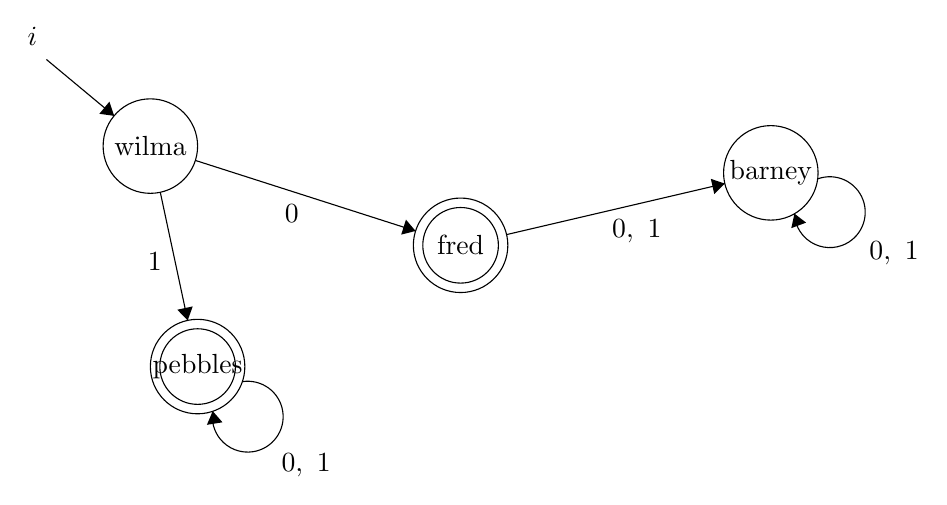
\begin{tikzpicture}[scale=0.2]
					\tikzstyle{every node}+=[inner sep=0pt]
					\draw [black] (17.3,-17.3) circle (3);
					\draw (17.3,-17.3) node {wilma};
					\draw [black] (37,-23.6) circle (3);
					\draw (37,-23.6) node {fred};
					\draw [black] (37,-23.6) circle (2.4);
					\draw [black] (56.7,-19) circle (3);
					\draw (56.7,-19) node {barney};
					\draw [black] (20.3,-31.3) circle (3);
					\draw (20.3,-31.3) node {pebbles};
					\draw [black] (20.3,-31.3) circle (2.4);
					\draw [black] (10.7,-11.8) -- (15,-15.38);
					\draw (10.15,-10.36) node [left] {$i$};
					\fill [black] (15,-15.38) -- (14.7,-14.48) -- (14.06,-15.25);
					\draw [black] (20.16,-18.21) -- (34.14,-22.69);
					\fill [black] (34.14,-22.69) -- (33.53,-21.97) -- (33.23,-22.92);
					\draw (26.28,-20.99) node [below] {$0$};
					\draw [black] (17.93,-20.23) -- (19.67,-28.37);
					\fill [black] (19.67,-28.37) -- (19.99,-27.48) -- (19.01,-27.69);
					\draw (18.05,-24.65) node [left] {$1$};
					\draw [black] (23.13,-32.26) arc (99:-189:2.25);
					\draw (25.6,-37.55) node [right] {$0,\mbox{ }1$};
					\fill [black] (21.26,-34.13) -- (20.89,-35) -- (21.88,-34.84);
					\draw [black] (39.92,-22.92) -- (53.78,-19.68);
					\fill [black] (53.78,-19.68) -- (52.89,-19.38) -- (53.11,-20.35);
					\draw (48.19,-21.95) node [below] {$0,\mbox{ }1$};
					\draw [black] (59.663,-19.386) arc (110.30993:-177.69007:2.25);
					\draw (62.93,-24.08) node [right] {$0,\mbox{ }1$};
					\fill [black] (58.2,-21.59) -- (58,-22.51) -- (58.94,-22.16);
				\end{tikzpicture}
			\end{center}

			You follow the arrows through the states, as necessary, and if you end up on a final state then the string is in the language.
			\\ \\
			We prefer total functions to partial functions. We add a new state, which we'll call ``barney,'' that acts as a black hole. A finite automaton only needs one black hole, where all transitions loop back to the black hole itself. We can always make $T$ total by directing transitions that are not otherwise specified to the black hole. The black hole state is \emph{not} a final state.
			\\ \\
			We can name our states whatever we'd like on our bubble diagram. Intelligent names should be chosen, like ``start,'' ``zero,'' ``nonzero,'' and ``fail,'' for instance.
			\\ \\
			Fun fact: regular languages have been proven to be closed under intersection and set difference. \lecture{February 6, 2013}
			\\ \\
			We sometimes denote a DFA as $\text{DFA} = < \Sigma, S, i, f, T >$.
			\\ \\
			For simplicity's sake, we'll setup some notation we'll be using to discuss DFAs. This is by convention only.
			\begin{itemize}
				\item $a, b, c, d$ (and other letters at the beginning of the standard alphabet) represent symbols in $\Sigma = \set{a, b, c, d}$.
				\item Particular strings are a concatenation of symbols from $\Sigma$. Some examples are $abca, bbca,$ and $\epsilon$ (the empty string).
				\item $x, y, z$ (and other letters near the end of the standard alphabet) are variables that represent strings. For example, let $x = abc$, then $x = x_0 x_1 x_2 \ldots x_{n - 1}$ where $n = |x|$.
			\end{itemize}
			The \textbf{DFA algorithm} is pretty simple. Given an input $x$ (which is implicitly a DFA = $< \Sigma, S, i, f, T >$, where $T$ is a total function), the output of the algorithm will be:
			\begin{align*}
				\begin{cases}
					\text{``accept''} & x \in L \\
					\text{``reject''} & x \not \in L
				\end{cases}
			\end{align*}
			The DFA algorithm is as follows: \\ \\
			\begin{algorithm}[H]
				state = i\;
				\For{$a = x_0, x_1, x_2, \ldots, x_{n - 1}$}{
					state = T[state, a]\;
				}
				\lIf{state $\in $ f}{accept}
				\lElse{reject}
			\end{algorithm}
			\vspace{0.5cm}
			The bonus question on A5 involves implementing this algorithm. You may want to use an array or map. It's the easiest bonus question all term.

			\begin{ex}
				We're given the binary integers, $\Sigma = \set{0, 1}, S = \set{\text{start}, \text{zero}, \text{nonzero}, \text{error}}, i = \text{start}, f = \set{\text{zero}, \text{nonzero}}$, and function $T$ defined by: \\
				\begin{center}
					\begin{tabular}{|c|c|}
						\hline $S \times \Sigma$ & $S$ \\ \hline
						start, 0 & zero \\
						start, 1 & nonzero \\
						zero, 0 & error \\
						zero, 1 & error \\
						nonzero, 0 & nonzero \\
						nonzero, 1 & nonzero \\
						error, 0 & error \\
						error, 1 & error \\ \hline
					\end{tabular}
				\end{center}
				This table for $T$ isn't very intuitive. Let's look at the bubble diagram representing this DFA for a clearer picture.

				\begin{center}
					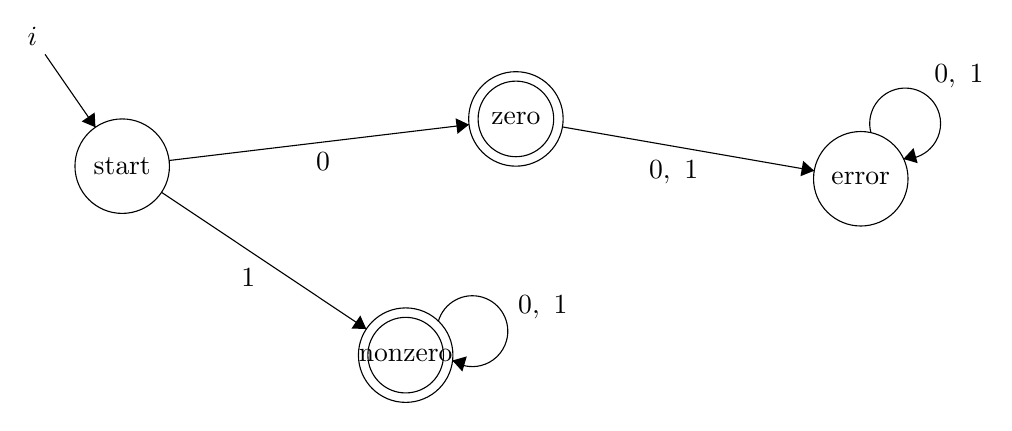
\begin{tikzpicture}[scale=0.2]
						\tikzstyle{every node}+=[inner sep=0pt]
						\draw [black] (13,-15.7) circle (3);
						\draw (13,-15.7) node {start};
						\draw [black] (38,-12.7) circle (3);
						\draw (38,-12.7) node {zero};
						\draw [black] (38,-12.7) circle (2.4);
						\draw [black] (59.9,-16.5) circle (3);
						\draw (59.9,-16.5) node {error};
						\draw [black] (31,-27.7) circle (3);
						\draw (31,-27.7) node {nonzero};
						\draw [black] (31,-27.7) circle (2.4);
						\draw [black] (15.5,-17.36) -- (28.5,-26.04);
						\fill [black] (28.5,-26.04) -- (28.12,-25.18) -- (27.56,-26.01);
						\draw (21,-22.2) node [below] {$1$};
						\draw [black] (33.075,-25.549) arc (163.75996:-124.24004:2.25);
						\draw (38.11,-24.64) node [right] {$0,\mbox{ }1$};
						\fill [black] (33.97,-28.04) -- (34.6,-28.74) -- (34.88,-27.78);
						\draw [black] (15.98,-15.34) -- (35.02,-13.06);
						\fill [black] (35.02,-13.06) -- (34.17,-12.66) -- (34.29,-13.65);
						\draw (25.76,-14.79) node [below] {$0$};
						\draw [black] (40.96,-13.21) -- (56.94,-15.99);
						\fill [black] (56.94,-15.99) -- (56.24,-15.36) -- (56.07,-16.34);
						\draw (48.02,-15.29) node [below] {$0,\mbox{ }1$};
						\draw [black] (60.547,-13.583) arc (195.22332:-92.77668:2.25);
						\draw (66.13,-10.74) node [above] {$0,\mbox{ }1$};
						\fill [black] (62.61,-15.24) -- (63.51,-15.51) -- (63.25,-14.55);
						\draw [black] (8.1,-8.6) -- (11.3,-13.23);
						\draw (7.3,-8.1) node [above] {$i$};
						\fill [black] (11.3,-13.23) -- (11.25,-12.29) -- (10.43,-12.86);
					\end{tikzpicture}
				\end{center}

				Let's look at \underline{x = 10}. x = 10 will execute the following: \\
				\begin{algorithm}[H]
					state = start\;
					state = T[start, 1]; // state = nonzero \\
					state = T[nonzero, 0]; // state = nonzero \\
					(end loop) \\
					nonzero $\in $ f? Yes, accept.
				\end{algorithm}
				\vspace{0.5cm}
				Next, let's look at \underline{x = 01}. x = 01 will execute the following: \\
				\begin{algorithm}[H]
					state = start\;
					state = T[start, 0]; // state = zero \\
					state = T[zero, 1]; // state = error \\
					(end loop) \\
					error $\in $ f? No, reject.
				\end{algorithm}
			\end{ex}

			\begin{ex}
				Let's construct a finite automaton that represents the MIPS assembly notation for registers.
				\\ \\
				Given $\Sigma = \set{\$, 0, 1, 2, 3, 4, 5, 6, 7, 8, 9}, L = $ MIPS assembly notation for registers (i.e. $\set{\$0, \$1, \$2, \ldots, \$31}$).
				\\ \\
				It's useful to name your DFA states with what you've learned so far based on the conditions that led to that state, because that's the only way we know what we've determined in the past. These names don't matter, but it'll make the finite automaton much easier for you to understand.
				\\ \\
				We're going to assume there is an error (black hole) state that all undefined transitions lead to. We'll make this assumption in general in this course. You need to draw the error state only when you need a \emph{total} function $T$ (such as when you intend to run the DFA algorithm), or when you're explicitly asked to draw it.
				\\ \\
				Let's look at the bubble diagram for this finite automaton that represents the notation of MIPS registers.
				\begin{center}
					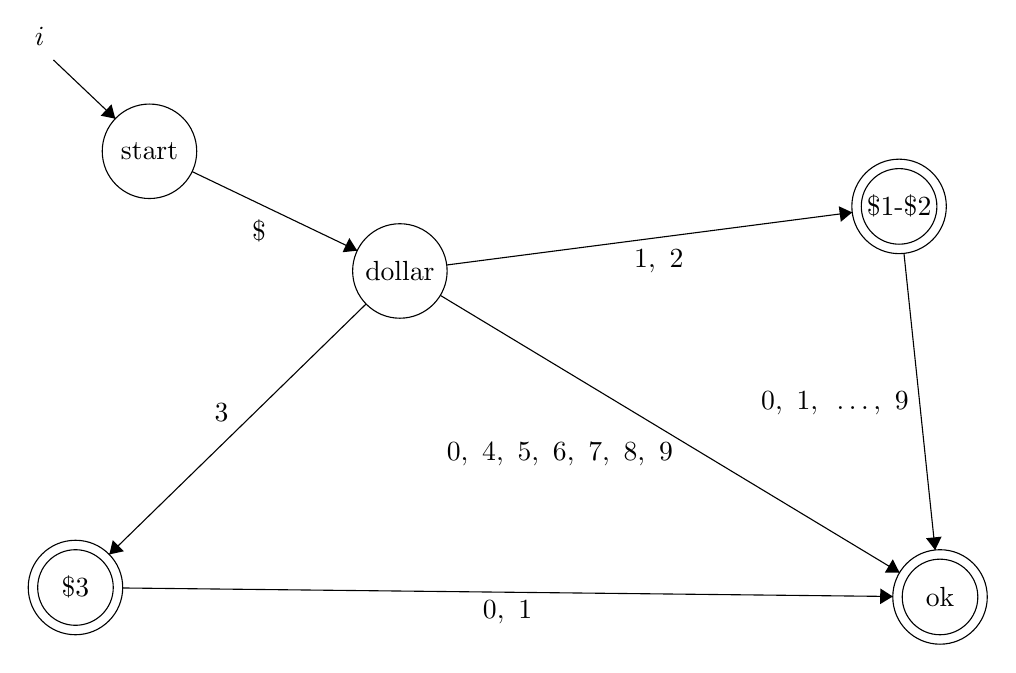
\begin{tikzpicture}[scale=0.2]
						\tikzstyle{every node}+=[inner sep=0pt]
						\draw [black] (11.8,-10.2) circle (3);
						\draw (11.8,-10.2) node {start};
						\draw [black] (27.7,-17.8) circle (3);
						\draw (27.7,-17.8) node {dollar};
						\draw [black] (62,-38.5) circle (3);
						\draw (62,-38.5) node {ok};
						\draw [black] (62,-38.5) circle (2.4);
						\draw [black] (59.4,-13.7) circle (3);
						\draw (59.4,-13.7) node {\$1-\$2};
						\draw [black] (59.4,-13.7) circle (2.4);
						\draw [black] (7.1,-37.9) circle (3);
						\draw (7.1,-37.9) node {\$3};
						\draw [black] (7.1,-37.9) circle (2.4);
						\draw [black] (5.7,-4.4) -- (9.63,-8.13);
						\draw (5.17,-2.93) node [left] {$i$};
						\fill [black] (9.63,-8.13) -- (9.39,-7.22) -- (8.7,-7.94);
						\draw [black] (14.51,-11.49) -- (24.99,-16.51);
						\fill [black] (24.99,-16.51) -- (24.49,-15.71) -- (24.06,-16.61);
						\draw (18.76,-14.51) node [below] {\$};
						\draw [black] (59.71,-16.68) -- (61.69,-35.52);
						\fill [black] (61.69,-35.52) -- (62.1,-34.67) -- (61.11,-34.77);
						\draw (60.05,-26.2) node [left] {$0,\mbox{ }1,\mbox{ }\dots,\mbox{ }9$};
						\draw [black] (10.1,-37.93) -- (59,-38.47);
						\fill [black] (59,-38.47) -- (58.21,-37.96) -- (58.19,-38.96);
						\draw (34.54,-38.72) node [below] {$0,\mbox{ }1$};
						\draw [black] (25.55,-19.9) -- (9.25,-35.8);
						\fill [black] (9.25,-35.8) -- (10.17,-35.6) -- (9.47,-34.89);
						\draw (16.38,-27.37) node [above] {$3$};
						\draw [black] (30.68,-17.42) -- (56.42,-14.08);
						\fill [black] (56.42,-14.08) -- (55.57,-13.69) -- (55.7,-14.68);
						\draw (44.14,-16.43) node [below] {$1,\mbox{ }2$};
						\draw [black] (30.27,-19.35) -- (59.43,-36.95);
						\fill [black] (59.43,-36.95) -- (59,-36.11) -- (58.49,-36.96);
						\draw (37.86,-28.66) node [below] {$0,\mbox{ }4,\mbox{ }5,\mbox{ }6,\mbox{ }7,\mbox{ }8,\mbox{ }9$};
					\end{tikzpicture}
				\end{center}

				Every MIPS register must start with the dollar sign (\$). Keep in mind that only $\$0, \ldots, \$31$ are valid MIPS registers. So, if the next number is a 1 or a 2, we can have any second digit (from 0-9) to form a valid MIPS register. If the number is 3, we can only follow that up by a 0 or 1 (\$30 and \$31). We also need to handle all other single digit registers (\$0, \$4, \$5, \$6, \$7, \$8, \$9).
				\\ \\
				We could've made this differently by having multiple ``ok'' states, but those aren't necessary so all valid registers point to the same ``ok'' state in this diagram. We can point all complete paths to a single complete state because what happens from the complete state onwards does not differ. In this case, all complete states have no further path (except to an implied black hole), and all complete states are final states, so having one complete state (denoted ``ok'' on the bubble diagram) is acceptable.
				\\ \\
				In general, you can combine two states if everything that follows from that point is the same among all of the states you're combining.
			\end{ex}

			\begin{ex}
				Let $\Sigma = \set{a, b, c}, L = $ any string with an odd number of $a$'s. For example: $a, abaa, babbc, \ldots$.
				\begin{center}
					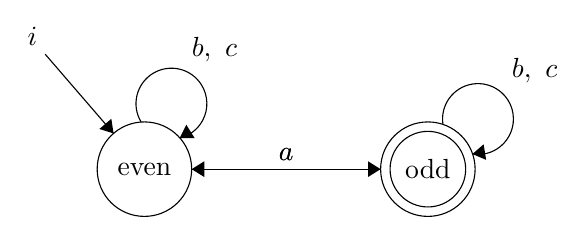
\begin{tikzpicture}[scale=0.2]
						\tikzstyle{every node}+=[inner sep=0pt]
						\draw [black] (21.7,-12.5) circle (3);
						\draw (21.7,-12.5) node {even};
						\draw [black] (39.7,-12.5) circle (3);
						\draw (39.7,-12.5) node {odd};
						\draw [black] (39.7,-12.5) circle (2.4);
						\draw [black] (15.4,-5.2) -- (19.74,-10.23);
						\draw (14.59,-4.71) node [above] {$i$};
						\fill [black] (19.74,-10.23) -- (19.6,-9.3) -- (18.84,-9.95);
						\draw [black] (21.499,-9.518) arc (211.59369:-76.40631:2.25);
						\draw (26.15,-5.73) node [above] {$b,\mbox{ }c$};
						\fill [black] (23.94,-10.53) -- (24.89,-10.53) -- (24.36,-9.68);
						\draw [black] (24.7,-12.5) -- (36.7,-12.5);
						\fill [black] (36.7,-12.5) -- (35.9,-12) -- (35.9,-13);
						\draw (30.7,-12) node [above] {$a$};
						\draw [black] (36.7,-12.5) -- (24.7,-12.5);
						\fill [black] (24.7,-12.5) -- (25.5,-13) -- (25.5,-12);
						\draw (30.7,-12) node [above] {$a$};
						\draw [black] (40.66,-9.67) arc (189:-99:2.25);
						\draw (45,-6.25) node [right] {$b,\mbox{ }c$};
						\fill [black] (42.53,-11.54) -- (43.4,-11.91) -- (43.24,-10.92);
					\end{tikzpicture}
				\end{center}
				(Note that there are two arrows between those nodes: one for each direction.)
				\\ \\
				We can keep track of one binary bit of information with a state. In this case, that bit is ``do I have an even number of $a$'s?''
				\\ \\
				Suppose instead we want $L = $ any string with an even number of $a$'s. That's the complement of $L$ from before.
				\\ \\
				To find the complement of a DFA, you make all non-finish states into finish states, and vice versa. That means the error (black hole) state will become a finish state as well.
				\begin{center}
					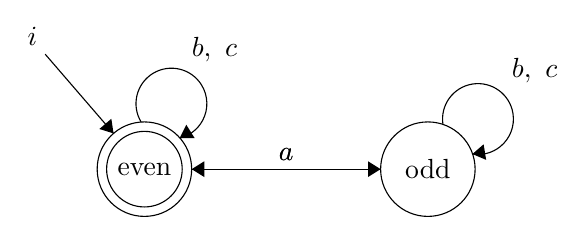
\begin{tikzpicture}[scale=0.2]
						\tikzstyle{every node}+=[inner sep=0pt]
						\draw [black] (21.7,-12.5) circle (3);
						\draw (21.7,-12.5) node {even};
						\draw [black] (21.7,-12.5) circle (2.4);
						\draw [black] (39.7,-12.5) circle (3);
						\draw (39.7,-12.5) node {odd};
						\draw [black] (15.4,-5.2) -- (19.74,-10.23);
						\draw (14.59,-4.71) node [above] {$i$};
						\fill [black] (19.74,-10.23) -- (19.6,-9.3) -- (18.84,-9.95);
						\draw [black] (21.499,-9.518) arc (211.59369:-76.40631:2.25);
						\draw (26.15,-5.73) node [above] {$b,\mbox{ }c$};
						\fill [black] (23.94,-10.53) -- (24.89,-10.53) -- (24.36,-9.68);
						\draw [black] (24.7,-12.5) -- (36.7,-12.5);
						\fill [black] (36.7,-12.5) -- (35.9,-12) -- (35.9,-13);
						\draw (30.7,-12) node [above] {$a$};
						\draw [black] (36.7,-12.5) -- (24.7,-12.5);
						\fill [black] (24.7,-12.5) -- (25.5,-13) -- (25.5,-12);
						\draw (30.7,-12) node [above] {$a$};
						\draw [black] (40.66,-9.67) arc (189:-99:2.25);
						\draw (45,-6.25) node [right] {$b,\mbox{ }c$};
						\fill [black] (42.53,-11.54) -- (43.4,-11.91) -- (43.24,-10.92);
					\end{tikzpicture}
				\end{center}
			\end{ex}

			\begin{ex}
				Let $\Sigma = \set{a, b, c}$ and $L$ = all strings with at least one $a$, one $b$, and one $c$. For example: $abaaaaaca \in L$, but $bcbcbccc \not \in L$.

				\begin{center}
					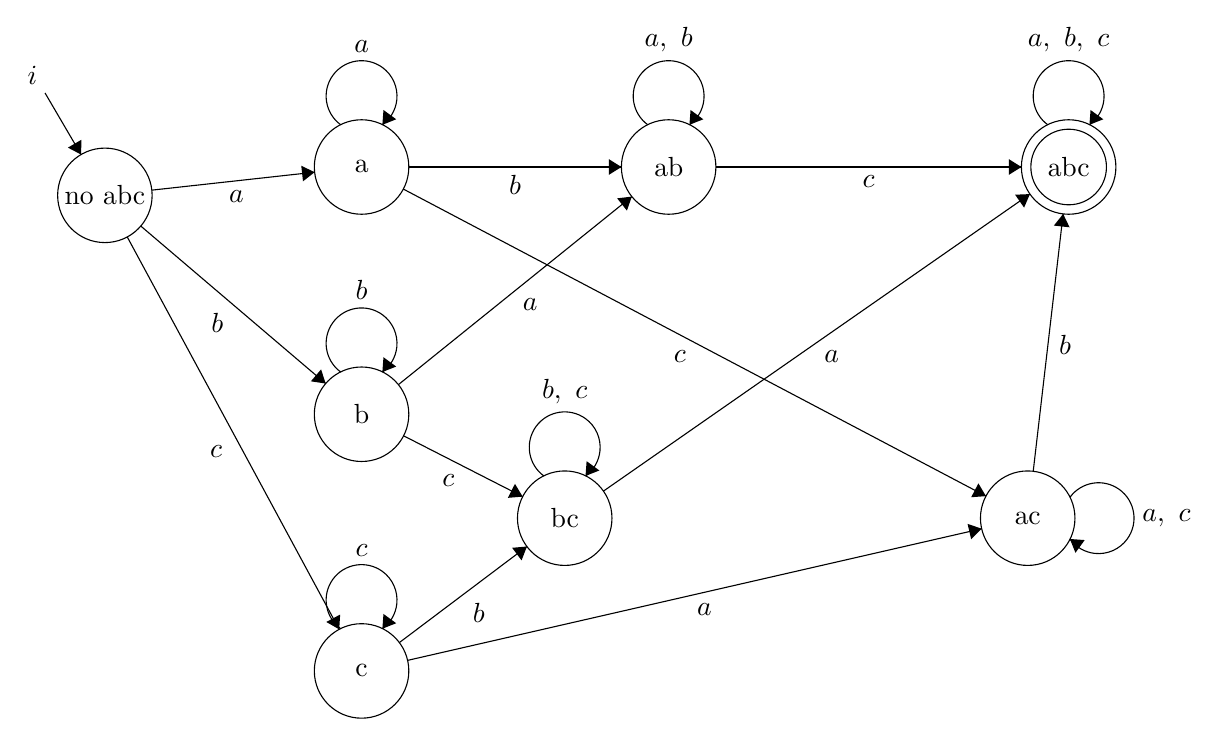
\begin{tikzpicture}[scale=0.2]
						\tikzstyle{every node}+=[inner sep=0pt]
						\draw [black] (8.5,-13.7) circle (3);
						\draw (8.5,-13.7) node {no abc};
						\draw [black] (24.8,-11.9) circle (3);
						\draw (24.8,-11.9) node {a};
						\draw [black] (24.8,-27.6) circle (3);
						\draw (24.8,-27.6) node {b};
						\draw [black] (24.8,-43.9) circle (3);
						\draw (24.8,-43.9) node {c};
						\draw [black] (44.3,-11.9) circle (3);
						\draw (44.3,-11.9) node {ab};
						\draw [black] (67.1,-34.2) circle (3);
						\draw (67.1,-34.2) node {ac};
						\draw [black] (69.7,-11.9) circle (3);
						\draw (69.7,-11.9) node {abc};
						\draw [black] (69.7,-11.9) circle (2.4);
						\draw [black] (37.7,-34.2) circle (3);
						\draw (37.7,-34.2) node {bc};
						\draw [black] (4.7,-7.2) -- (6.99,-11.11);
						\draw (3.9,-6.7) node [above] {$i$};
						\fill [black] (6.99,-11.11) -- (7.01,-10.17) -- (6.15,-10.67);
						\draw [black] (11.48,-13.37) -- (21.82,-12.23);
						\fill [black] (21.82,-12.23) -- (20.97,-11.82) -- (21.08,-12.81);
						\draw (16.86,-13.38) node [below] {$a$};
						\draw [black] (10.78,-15.65) -- (22.52,-25.65);
						\fill [black] (22.52,-25.65) -- (22.23,-24.75) -- (21.58,-25.51);
						\draw (15.64,-21.14) node [below] {$b$};
						\draw [black] (9.92,-16.34) -- (23.38,-41.26);
						\fill [black] (23.38,-41.26) -- (23.44,-40.32) -- (22.56,-40.79);
						\draw (15.98,-29.98) node [left] {$c$};
						\draw [black] (23.477,-9.22) arc (234:-54:2.25);
						\draw (24.8,-4.65) node [above] {$a$};
						\fill [black] (26.12,-9.22) -- (27,-8.87) -- (26.19,-8.28);
						\draw [black] (23.477,-24.92) arc (234:-54:2.25);
						\draw (24.8,-20.35) node [above] {$b$};
						\fill [black] (26.12,-24.92) -- (27,-24.57) -- (26.19,-23.98);
						\draw [black] (23.477,-41.22) arc (234:-54:2.25);
						\draw (24.8,-36.65) node [above] {$c$};
						\fill [black] (26.12,-41.22) -- (27,-40.87) -- (26.19,-40.28);
						\draw [black] (27.72,-43.23) -- (64.18,-34.87);
						\fill [black] (64.18,-34.87) -- (63.28,-34.56) -- (63.51,-35.54);
						\draw (46.58,-39.62) node [below] {$a$};
						\draw [black] (68.377,-9.22) arc (234:-54:2.25);
						\draw (69.7,-4.65) node [above] {$a,\mbox{ }b,\mbox{ }c$};
						\fill [black] (71.02,-9.22) -- (71.9,-8.87) -- (71.09,-8.28);
						\draw [black] (27.2,-42.1) -- (35.3,-36);
						\fill [black] (35.3,-36) -- (34.36,-36.08) -- (34.96,-36.88);
						\draw (32.25,-39.55) node [below] {$b$};
						\draw [black] (27.47,-28.97) -- (35.03,-32.83);
						\fill [black] (35.03,-32.83) -- (34.54,-32.02) -- (34.09,-32.91);
						\draw (30.31,-31.4) node [below] {$c$};
						\draw [black] (27.45,-13.3) -- (64.45,-32.8);
						\fill [black] (64.45,-32.8) -- (63.97,-31.99) -- (63.51,-32.87);
						\draw (45.01,-23.55) node [below] {$c$};
						\draw [black] (27.8,-11.9) -- (41.3,-11.9);
						\fill [black] (41.3,-11.9) -- (40.5,-11.4) -- (40.5,-12.4);
						\draw (34.55,-12.4) node [below] {$b$};
						\draw [black] (42.977,-9.22) arc (234:-54:2.25);
						\draw (44.3,-4.65) node [above] {$a,\mbox{ }b$};
						\fill [black] (45.62,-9.22) -- (46.5,-8.87) -- (45.69,-8.28);
						\draw [black] (36.377,-31.52) arc (234:-54:2.25);
						\draw (37.7,-26.95) node [above] {$b,\mbox{ }c$};
						\fill [black] (39.02,-31.52) -- (39.9,-31.17) -- (39.09,-30.58);
						\draw [black] (27.14,-25.72) -- (41.96,-13.78);
						\fill [black] (41.96,-13.78) -- (41.03,-13.89) -- (41.65,-14.67);
						\draw (35.51,-20.24) node [below] {$a$};
						\draw [black] (47.3,-11.9) -- (66.7,-11.9);
						\fill [black] (66.7,-11.9) -- (65.9,-11.4) -- (65.9,-12.4);
						\draw (57,-12.4) node [below] {$c$};
						\draw [black] (67.45,-31.22) -- (69.35,-14.88);
						\fill [black] (69.35,-14.88) -- (68.76,-15.62) -- (69.76,-15.73);
						\draw (69.06,-23.17) node [right] {$b$};
						\draw [black] (40.16,-32.48) -- (67.24,-13.62);
						\fill [black] (67.24,-13.62) -- (66.3,-13.66) -- (66.87,-14.48);
						\draw (54.65,-23.55) node [below] {$a$};
						\draw [black] (69.78,-32.877) arc (144:-144:2.25);
						\draw (74.35,-34.2) node [right] {$a,\mbox{ }c$};
						\fill [black] (69.78,-35.52) -- (70.13,-36.4) -- (70.72,-35.59);
					\end{tikzpicture}
				\end{center}

				$T$ in this case is a total function. It has eight states because we need to keep track of three binary facts, which requires three bits of information ($2^3 = 8$).
			\end{ex}
			Similarly, if we had a DFA to determine if every letter in the English alphabet is included in a particular string, we would need $2^{26}$ states because we would need to store 26 bits of information. At some point, we say a number is large enough that \emph{in practice} we can treat it as an infinite number, despite it being finite. We wouldn't solve this problem with a DFA because $2^{26}$ is a number large enough that we wouldn't want to create a state for each of them.
		\subsubsection{Searching and Scanning with DFAs} \lecture{February 11, 2013}
			\begin{itemize}
				\item \textbf{Recognition} answers the question ``is $x \in L$?'' This is what we've used DFAs for so far.
				\item \textbf{Search} answers the question ``does $x$ contain $y \in L$?''. More formally, Does $\exists w, y, z . x = wyz$ and $y \in L$?
				\item \textbf{Find} answers the question ``where in $x$ is $y \in L$'' (where $x = x_0 x_1 \ldots x_{|x|-1}$)? This question could have multiple answers, depending on what you're asked for, such as:
					\begin{itemize}
						\item $y$ begins at $x_i$.
						\item $y$ ends at $x_j$.
						\item $y$ begins at $x_i$ and ends at $x_j$. This can be expressed as the pair $(i, j)$.
					\end{itemize}

					Find is a more general result than search.
				\item \textbf{Scan} partitions $x$ into $x = y_0 y_1 y_2 y_3 \ldots y_n$ and $\forall i y_i \in L$.
			\end{itemize}

			\begin{ex}
				Let $\Sigma = \set{a, b, c, 0, 1, 2, !}$ be an alphabet. We're interested in $L_{\text{id}}$ \textendash{} that is, the language of identifiers.
				\\ \\
				We can determine a \underline{recognizer} for $L_{\text{id}}$:
				\begin{center}
					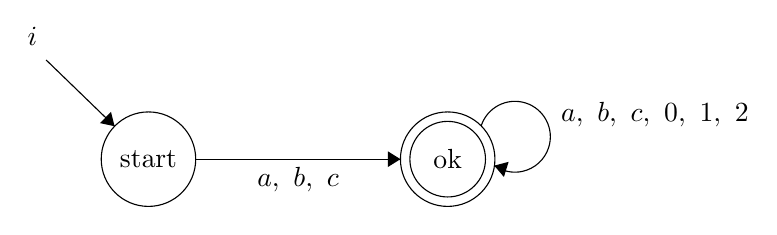
\begin{tikzpicture}[scale=0.2]
						\tikzstyle{every node}+=[inner sep=0pt]
						\draw [black] (18.5,-22.9) circle (3);
						\draw (18.5,-22.9) node {start};
						\draw [black] (37.5,-22.9) circle (3);
						\draw (37.5,-22.9) node {ok};
						\draw [black] (37.5,-22.9) circle (2.4);
						\draw [black] (12,-16.6) -- (16.35,-20.81);
						\draw (11.47,-15.13) node [left] {$i$};
						\fill [black] (16.35,-20.81) -- (16.12,-19.9) -- (15.42,-20.61);
						\draw [black] (21.5,-22.9) -- (34.5,-22.9);
						\fill [black] (34.5,-22.9) -- (33.7,-22.4) -- (33.7,-23.4);
						\draw (28,-23.4) node [below] {$a,\mbox{ }b,\mbox{ }c$};
						\draw [black] (39.624,-20.798) arc (162.43495:-125.56505:2.25);
						\draw (44.67,-20.06) node [right] {$a,\mbox{ }b,\mbox{ }c,\mbox{ }0,\mbox{ }1,\mbox{ }2$};
						\fill [black] (40.46,-23.31) -- (41.07,-24.03) -- (41.37,-23.07);
					\end{tikzpicture}
				\end{center}

				\underline{Searching} for $L_{\text{id}}$ in $x$, where $x = !abc!cba!$ yields the vacuous result of ``yes!'' There is an identifier in $x$, somewhere.
				\\ \\
				Some possible answers for \underline{find} include:
				\begin{itemize}
					\item $i = 1$ is the start of $y \in L$.
					\item $i = 5$ is the start of $y \in L$.
					\item $j = 3$ is the end of $y \in L$.
					\item $j = 7$ is the end of $y \in L$.
					\item $(i, j) = (1, 3)$ is $y \in L$.
					\item $(i, j) = (5, 7)$ is $y \in L$.
				\end{itemize}

				Those are not the only answers for find, however. ``bc'' is a valid identifier, and it's contained within $x$. So, we have a number of additional solutions:
				\begin{itemize}
					\item $i = 2$ is the start of $y \in L$.
					\item $i = 3$ is the start of $y \in L$.
					\item $j = 1$ is the end of $y \in L$.
					\item $j = 2$ is the end of $y \in L$.
					\item etc.
				\end{itemize}

				There are $O(|x|)$ possible solutions that indicate where $y \in L$ either begins or ends. There are also many additional pair solutions for the same reason:
				\begin{itemize}
					\item $(i, j) = (1, 1)$ is $y \in L$.
					\item $(i, j) = (1, 2)$ is $y \in L$.
					\item $(i, j) = (1, 3)$ is $y \in L$.
					\item $(i, j) = (5, 5)$ is $y \in L$.
					\item $(i, j) = (5, 6)$ is $y \in L$.
					\item $(i, j) = (6, 7)$ is $y \in L$.
					\item etc.
				\end{itemize}

				There are $O(|x^2|)$ possible $(i, j)$ pair solutions.
			\end{ex}
			We would like to specify a \underline{unique} solution. How could we do this? First, you have to choose whether you want $i$, $j$, or $(i, j)$ as the format of your solution. If you want just $i$ or $j$, then simply pick the first solution. But if you want the pair $(i, j)$, ``first'' is ill-defined. For example: does $(10, 20)$ come before $(5, 25)$? There's no correct answer, it's all about definitions.
			\\ \\
			The most common choice for a unique solution is to use the leftmost longest match.
			\begin{defn}
				The \textbf{leftmost longest match} is found by finding $(i, j)$ such that $x_i x_{i + 1} \ldots x_j \in L$, $i$ is minimized, and given $i$, $j$ is maximized.
			\end{defn}
			A subproblem of the leftmost longest match algorithm is the longest prefix problem.
			\begin{defn}
				The \textbf{longest prefix problem} is when given $x$, find the longest prefix (of $x$), $y \in L$.
			\end{defn}

			For example, if $x = abc123!abc$, the longest prefix is $abc123$. This can be identified by $j$, where $x_j$ is the end of the prefix of $y$.
			\begin{ex}
				Suppose $L = \set{a, aaa}$. Let's find the longest match.
				\\ \\
				If we have $x = aa\ldots$, after we examine the first $a$, we have no idea if that's the longest match or not. Only after examining more of the string can we be sure that it is. In $aab$, $a$ is the longest match. In $aaa$, $aaa$ is the longest match and so $a$ is not the longest match.
			\end{ex}

			\begin{ex}
				Suppose $L = \set{a} \cup \set{\text{any string beginning with } a \text{ and ending in } b}$. We can determine a recognizer for this:
				\begin{center}
				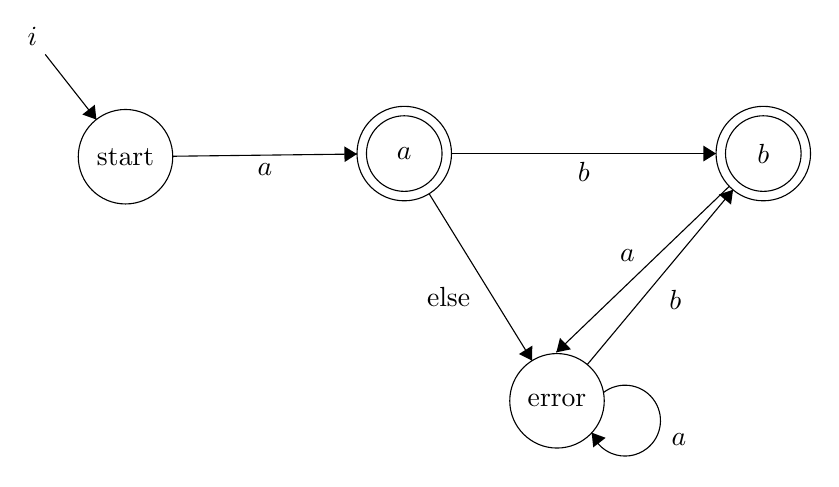
\begin{tikzpicture}[scale=0.2]
				\tikzstyle{every node}+=[inner sep=0pt]
				\draw [black] (10.3,-20.6) circle (3);
				\draw (10.3,-20.6) node {start};
				\draw [black] (28,-20.4) circle (3);
				\draw (28,-20.4) node {$a$};
				\draw [black] (28,-20.4) circle (2.4);
				\draw [black] (50.8,-20.4) circle (3);
				\draw (50.8,-20.4) node {$b$};
				\draw [black] (50.8,-20.4) circle (2.4);
				\draw [black] (37.7,-36.1) circle (3);
				\draw (37.7,-36.1) node {error};
				\draw [black] (5.2,-14.1) -- (8.45,-18.24);
				\draw (4.39,-13.6) node [above] {$i$};
				\fill [black] (8.45,-18.24) -- (8.35,-17.3) -- (7.56,-17.92);
				\draw [black] (13.3,-20.57) -- (25,-20.43);
				\fill [black] (25,-20.43) -- (24.19,-19.94) -- (24.21,-20.94);
				\draw (19.15,-21.01) node [below] {$a$};
				\draw [black] (31,-20.4) -- (47.8,-20.4);
				\fill [black] (47.8,-20.4) -- (47,-19.9) -- (47,-20.9);
				\draw (39.4,-20.9) node [below] {$b$};
				\draw [black] (29.58,-22.95) -- (36.12,-33.55);
				\fill [black] (36.12,-33.55) -- (36.13,-32.6) -- (35.28,-33.13);
				\draw (32.22,-29.53) node [left] {else};
				\draw [black] (39.62,-33.8) -- (48.88,-22.7);
				\fill [black] (48.88,-22.7) -- (47.98,-23) -- (48.75,-23.64);
				\draw (44.8,-29.69) node [right] {$b$};
				\draw [black] (40.643,-35.58) arc (127.75839:-160.24161:2.25);
				\draw (44.95,-38.57) node [right] {$a$};
				\fill [black] (39.9,-38.12) -- (40,-39.06) -- (40.79,-38.45);
				\draw [black] (48.64,-22.48) -- (37.66,-33.02);
				\fill [black] (37.66,-33.02) -- (38.59,-32.83) -- (37.89,-32.11);
				\draw (42.18,-27.27) node [above] {$a$};
				\end{tikzpicture}
				\end{center}

				If we have $x = acc012cca12\ldots$ and we're examining $a$ at the beginning, we're unsure if that's the longest prefix $y \in L$ yet. We have to continue looking to be sure.
			\end{ex}

			Here's the pseudocode for determining the longest prefix using a DFA, given an input $x = x_0 x_1 \ldots x_{|x|-1}$. \\
			\begin{algorithm}[H]
				state = start\;
				j = -1\;
				\For{i = 0 to |x| - 1}{
					\lIf{state $\in$ final}{j = i}
					state = T[state, $x_i$]\;
					// You could always hope\dots this is optional though: \\
					\lIf{state is black hole}{reject}
				}
				\lIf{$j \ge 0$}{accept, $y = x_0 \ldots x_{j - 1} \in L$}
				\lElse{reject}
			\end{algorithm}

			Next, let's take a deeper look at \underline{scanning}. With scanning, we want to partition $x$ using the longest prefix. This is also called leftmost longest, or more colloquially, the \textbf{maximal munch} scanning algorithm. \\
			\begin{algorithm}
				start with $x$\;
				\While{$x \ne \epsilon$}{
					find leftmost longest match of $L$\;
					report result $y$, remove $y$ from $x$\;
				}
			\end{algorithm}

			In this algorithm, $L$ is the language of all tokens and separators. That is, $L = L_{\text{id}} \cup L_{\text{int}} \cup L_{\text{!}}$, where $L_{\text{int}}$ has this recognizer:
			\begin{center}
				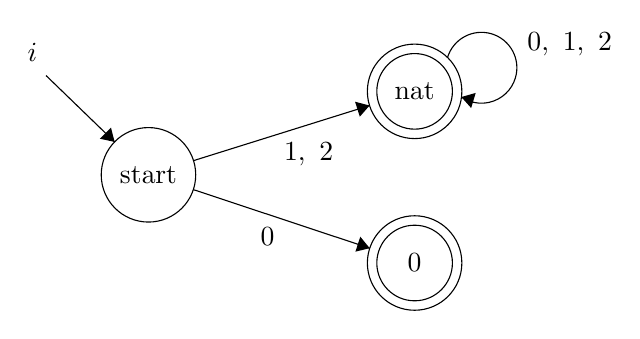
\begin{tikzpicture}[scale=0.2]
					\tikzstyle{every node}+=[inner sep=0pt]
					\draw [black] (18,-21.8) circle (3);
					\draw (18,-21.8) node {start};
					\draw [black] (34.9,-27.4) circle (3);
					\draw (34.9,-27.4) node {$0$};
					\draw [black] (34.9,-27.4) circle (2.4);
					\draw [black] (34.9,-16.5) circle (3);
					\draw (34.9,-16.5) node {nat};
					\draw [black] (34.9,-16.5) circle (2.4);
					\draw [black] (11.5,-15.5) -- (15.85,-19.71);
					\draw (10.97,-14.03) node [left] {$i$};
					\fill [black] (15.85,-19.71) -- (15.62,-18.8) -- (14.92,-19.51);
					\draw [black] (20.86,-20.9) -- (32.04,-17.4);
					\fill [black] (32.04,-17.4) -- (31.12,-17.16) -- (31.42,-18.11);
					\draw (28.17,-19.74) node [below] {$1,\mbox{ }2$};
					\draw [black] (36.987,-14.361) arc (163.44003:-124.55997:2.25);
					\draw (42.03,-13.5) node [right] {$0,\mbox{ }1,\mbox{ }2$};
					\fill [black] (37.87,-16.86) -- (38.49,-17.56) -- (38.78,-16.6);
					\draw [black] (20.85,-22.74) -- (32.05,-26.46);
					\fill [black] (32.05,-26.46) -- (31.45,-25.73) -- (31.14,-26.68);
					\draw (25.56,-25.14) node [below] {$0$};
				\end{tikzpicture}
			\end{center}

			And $L_{\text{!}}$ has this recognizer:
			\begin{center}
				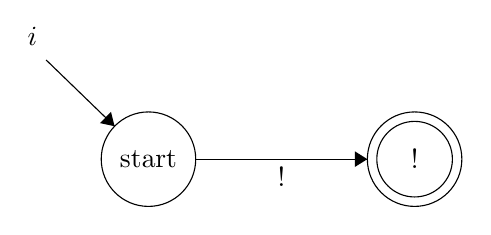
\begin{tikzpicture}[scale=0.2]
					\tikzstyle{every node}+=[inner sep=0pt]
					\draw [black] (18,-21.8) circle (3);
					\draw (18,-21.8) node {start};
					\draw [black] (34.9,-21.8) circle (3);
					\draw (34.9,-21.8) node {!};
					\draw [black] (34.9,-21.8) circle (2.4);
					\draw [black] (11.5,-15.5) -- (15.85,-19.71);
					\draw (10.97,-14.03) node [left] {$i$};
					\fill [black] (15.85,-19.71) -- (15.62,-18.8) -- (14.92,-19.51);
					\draw [black] (21,-21.8) -- (31.9,-21.8);
					\fill [black] (31.9,-21.8) -- (31.1,-21.3) -- (31.1,-22.3);
					\draw (26.45,-22.3) node [below] {$!$};
				\end{tikzpicture}
			\end{center}

			There is a problem with maximal munch \textendash{} efficiency.
			\\ \\
			\textbf{Runtime of Maximal Munch}: the loop executes $|x|$ times, and for each iteration, it uses the ``find largest prefix'' algorithm (which itself takes $O(|x|)$ time). $|x| \cdot O(|x|) \in O(|x|^2)$.
			\\ \\
			In order to improve efficiency and readability, we'll use a ``total hack'' called \textbf{simplified maximal munch}. This involves finding the longest prefix $y$ of $x$ such that $ya$ could not possibly be a prefix of $L$ where $x = yaz$.
			\\ \\
			Suppose you have $L_{\text{int}} = \set{0, 1, 2, 3, \ldots}, L_{\text{id}} = \set{x}$, and $L_{\text{hex}} = \set{0x1, \ldots}$. If you have $x = 0x$, you can't determine if that's the integer zero followed by an identifier, or the beginning of a hex symbol. However, if you can look ahead and see $0x1$, you know it's a hex symbol. If you see something like $0xx$ (a hex prefix followed by an identifier), simplified maximal munch will not allow this.
			\\ \\
			The scanner we were given (which implements simplified maximal munch) will see $0xx$ as an error. It's an error because the scanner made the assumption that it was a hex constant, but that didn't work out (didn't see an integer after 0x), so it gave up and produced an error.
		\subsection{Nondeterministic Finite Automata (NFA)} \lecture{February 13, 2013}
			\begin{ex}
				Let's say we have the alphabet $\Sigma = \set{a, b, c}$ and the language $L = \set{abc, abaca}$. A recognizer for this NFA could be drawn as:
				\begin{center}
					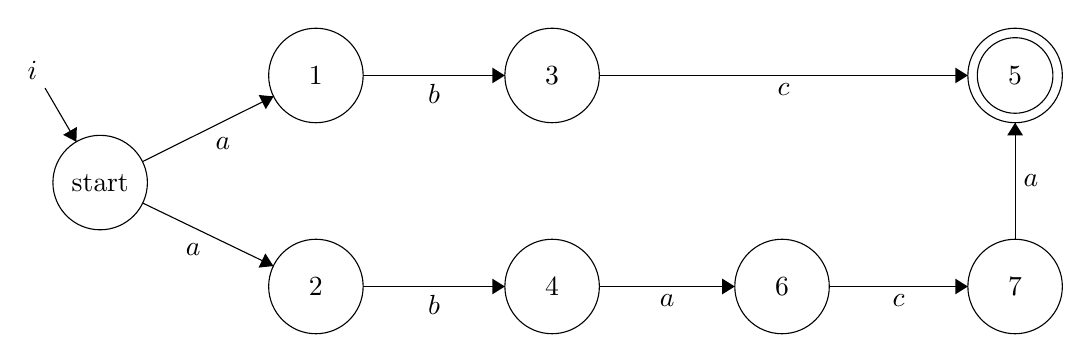
\begin{tikzpicture}[scale=0.2]
						\tikzstyle{every node}+=[inner sep=0pt]
						\draw [black] (8,-18.9) circle (3);
						\draw (8,-18.9) node {start};
						\draw [black] (21.7,-12.1) circle (3);
						\draw (21.7,-12.1) node {$1$};
						\draw [black] (36.7,-12.1) circle (3);
						\draw (36.7,-12.1) node {$3$};
						\draw [black] (66.1,-12.1) circle (3);
						\draw (66.1,-12.1) node {$5$};
						\draw [black] (66.1,-12.1) circle (2.4);
						\draw [black] (21.7,-25.5) circle (3);
						\draw (21.7,-25.5) node {$2$};
						\draw [black] (36.7,-25.5) circle (3);
						\draw (36.7,-25.5) node {$4$};
						\draw [black] (51.3,-25.5) circle (3);
						\draw (51.3,-25.5) node {$6$};
						\draw [black] (66.1,-25.5) circle (3);
						\draw (66.1,-25.5) node {$7$};
						\draw [black] (10.7,-20.2) -- (19,-24.2);
						\fill [black] (19,-24.2) -- (18.49,-23.4) -- (18.06,-24.3);
						\draw (13.91,-22.71) node [below] {$a$};
						\draw [black] (24.7,-25.5) -- (33.7,-25.5);
						\fill [black] (33.7,-25.5) -- (32.9,-25) -- (32.9,-26);
						\draw (29.2,-26) node [below] {$b$};
						\draw [black] (39.7,-25.5) -- (48.3,-25.5);
						\fill [black] (48.3,-25.5) -- (47.5,-25) -- (47.5,-26);
						\draw (44,-26) node [below] {$a$};
						\draw [black] (54.3,-25.5) -- (63.1,-25.5);
						\fill [black] (63.1,-25.5) -- (62.3,-25) -- (62.3,-26);
						\draw (58.7,-26) node [below] {$c$};
						\draw [black] (66.1,-22.5) -- (66.1,-15.1);
						\fill [black] (66.1,-15.1) -- (65.6,-15.9) -- (66.6,-15.9);
						\draw (66.6,-18.8) node [right] {$a$};
						\draw [black] (10.69,-17.57) -- (19.01,-13.43);
						\fill [black] (19.01,-13.43) -- (18.07,-13.34) -- (18.52,-14.24);
						\draw (15.79,-16) node [below] {$a$};
						\draw [black] (24.7,-12.1) -- (33.7,-12.1);
						\fill [black] (33.7,-12.1) -- (32.9,-11.6) -- (32.9,-12.6);
						\draw (29.2,-12.6) node [below] {$b$};
						\draw [black] (39.7,-12.1) -- (63.1,-12.1);
						\fill [black] (63.1,-12.1) -- (62.3,-11.6) -- (62.3,-12.6);
						\draw (51.4,-12.6) node [below] {$c$};
						\draw [black] (4.5,-12.9) -- (6.49,-16.31);
						\draw (3.7,-12.4) node [above] {$i$};
						\fill [black] (6.49,-16.31) -- (6.52,-15.37) -- (5.65,-15.87);
					\end{tikzpicture}
				\end{center}

				This is \underline{not} a DFA because T[start, a] = 1 and T[start, a] = 2, which is not allowed in a DFA. It is acceptable for an NFA, though.
				\label{ex:nfa}
			\end{ex}

			The transition function $T$ no longer has to be a function \textendash{} it can have multiple transition values for the same input symbols.
			\\ \\
			The rule is the same as before: if there is \underline{any} path that is followed to a finish state, then the string is considered to be in the language. With DFAs, we used the ``one-finger algorithm,'' but now we can't do that because there could be multiple paths we need to follow.
			\\ \\
			An \textbf{oracle} is a magic function in CS theory that sees the future. If you have an oracle then you could resolve the proper path and use the same process as a DFA. However, we don't have an oracle. When we see multiple paths, we clone our finger and follow each path as far as we can. This is more operationally satisfactory than looking into the future.
			\\ \\
			More formally, an $\text{NFA} = (\Sigma, S, i, f, T)$, where $\Sigma, S, i$, and $f$ follow the same definitions as with DFAs. However, $T: S \times \Sigma \to 2^S$ (where $2^S$ is the number of subsets of $S$). In \ref{ex:nfa}, we have that $T$ is defined by the table:
			\begin{center}
				\begin{tabular}{|c|c|}
					\hline
					start, a & $\set{1, 2}$ \\
					1, b & $\set{3}$ \\
					2, b & $\set{4}$ \\
					3, c & $\set{5}$ \\
					4, a & $\set{6}$ \\
					6, c & $\set{7}$ \\
					7, a & $\set{5}$ \\
					3, a & $\set{}$ \\ \hline
				\end{tabular}
			\end{center}
			Additionally, we have $\Sigma = \set{a, b, c}, i = start, S = \set{start, 1, 2, 3, 4, 5, 6, 7}$, and $f = \set{5}$.
			\\ \\
			Note that we no longer need an error state because we are no longer required to make $T$ a total function, since it is doesn't need to be a function at all.
			\\ \\
			\textbf{NFA recognizer}: given an input string $x$, we expect output to be:
			\begin{align*}
				\text{output} &= \begin{cases}
					\text{``accept''} & x \in L \\
					\text{``reject''} & x \not \in L
				\end{cases}
			\end{align*}

			The pseudocode for an NFA recognizer is as follows. \\
			\begin{algorithm}[H]
				states = $\set{start}$\;
				\For{a in $x_0x_1x_2 \ldots x_{|x|-1}$}{
					states = $\displaystyle \bigcup_{s \in \text{states}}$ T[s, a]\;
				}
				\lIf{$\text{states} \cap f \ne \set{}$}{``accept''}
				\lElse{``reject''}
			\end{algorithm}

			\begin{theorem}
				Any language recognized by an NFA can be recognized by a DFA.
			\end{theorem}

			\underline{Proof outline}: subset construction. For an $\text{NFA} = \set{\Sigma, S_{\text{NFA}}, i_{\text{NFA}}, f_{\text{NFA}}, T_{\text{NFA}}}$, we can construct a $\text{DFA} = \set{\Sigma, S_{\text{DFA}}, i_{\text{DFA}}, f_{\text{DFA}}, T_{\text{DFA}}}$. Why does this work?
			\begin{enumerate}
				\item $S_{\text{NFA}}$ is finite.
				\item The number of subsets of a finite set is finite. There are $2^{|S|}$ subsets of a finite set $S$.
				\item Each state in $S_{\text{DFA}}$ represents a subset of the states in $S_{\text{NFA}}$.
			\end{enumerate}

			From the NFA in \ref{ex:nfa}, we can create this corresponding DFA:
			\begin{center}
				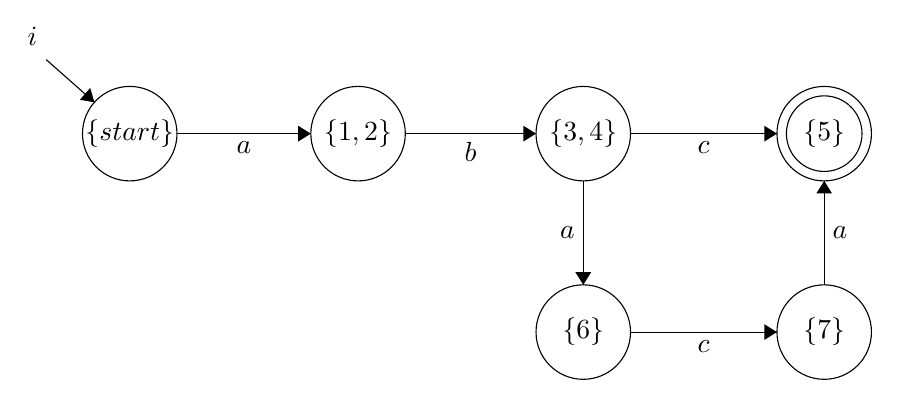
\begin{tikzpicture}[scale=0.2]
					\tikzstyle{every node}+=[inner sep=0pt]
					\draw [black] (12.7,-17.8) circle (3);
					\draw (12.7,-17.8) node {$\set{start}$};
					\draw [black] (27.2,-17.8) circle (3);
					\draw (27.2,-17.8) node {$\set{1, 2}$};
					\draw [black] (41.5,-17.8) circle (3);
					\draw (41.5,-17.8) node {$\set{3, 4}$};
					\draw [black] (56.8,-17.8) circle (3);
					\draw (56.8,-17.8) node {$\set{5}$};
					\draw [black] (56.8,-17.8) circle (2.4);
					\draw [black] (41.5,-30.4) circle (3);
					\draw (41.5,-30.4) node {$\set{6}$};
					\draw [black] (56.8,-30.4) circle (3);
					\draw (56.8,-30.4) node {$\set{7}$};
					\draw [black] (7.4,-13.1) -- (10.46,-15.81);
					\draw (6.86,-11.65) node [left] {$i$};
					\fill [black] (10.46,-15.81) -- (10.19,-14.9) -- (9.53,-15.65);
					\draw [black] (15.7,-17.8) -- (24.2,-17.8);
					\fill [black] (24.2,-17.8) -- (23.4,-17.3) -- (23.4,-18.3);
					\draw (19.95,-18.3) node [below] {$a$};
					\draw [black] (30.2,-17.8) -- (38.5,-17.8);
					\fill [black] (38.5,-17.8) -- (37.7,-17.3) -- (37.7,-18.3);
					\draw (34.35,-18.3) node [below] {$b$};
					\draw [black] (44.5,-17.8) -- (53.8,-17.8);
					\fill [black] (53.8,-17.8) -- (53,-17.3) -- (53,-18.3);
					\draw (49.15,-18.3) node [below] {$c$};
					\draw [black] (41.5,-20.8) -- (41.5,-27.4);
					\fill [black] (41.5,-27.4) -- (42,-26.6) -- (41,-26.6);
					\draw (41,-24.1) node [left] {$a$};
					\draw [black] (44.5,-30.4) -- (53.8,-30.4);
					\fill [black] (53.8,-30.4) -- (53,-29.9) -- (53,-30.9);
					\draw (49.15,-30.9) node [below] {$c$};
					\draw [black] (56.8,-27.4) -- (56.8,-20.8);
					\fill [black] (56.8,-20.8) -- (56.3,-21.6) -- (57.3,-21.6);
					\draw (57.3,-24.1) node [right] {$a$};
				\end{tikzpicture}
			\end{center}
		\subsection{Epsilon Nondeterministic Finite Automata ($\epsilon$-NFA)}
			\begin{ex}
				This is an example of an $\epsilon$-NFA:
				\begin{center}
					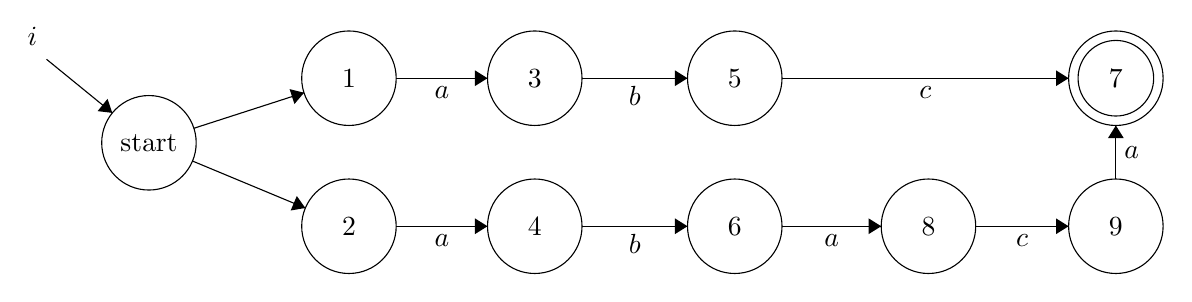
\begin{tikzpicture}[scale=0.2]
						\tikzstyle{every node}+=[inner sep=0pt]
						\draw [black] (12.6,-17.6) circle (3);
						\draw (12.6,-17.6) node {start};
						\draw [black] (25.3,-13.5) circle (3);
						\draw (25.3,-13.5) node {$1$};
						\draw [black] (37.1,-13.5) circle (3);
						\draw (37.1,-13.5) node {$3$};
						\draw [black] (49.8,-13.5) circle (3);
						\draw (49.8,-13.5) node {$5$};
						\draw [black] (74,-13.5) circle (3);
						\draw (74,-13.5) node {$7$};
						\draw [black] (74,-13.5) circle (2.4);
						\draw [black] (25.3,-22.9) circle (3);
						\draw (25.3,-22.9) node {$2$};
						\draw [black] (37.1,-22.9) circle (3);
						\draw (37.1,-22.9) node {$4$};
						\draw [black] (49.8,-22.9) circle (3);
						\draw (49.8,-22.9) node {$6$};
						\draw [black] (62.1,-22.9) circle (3);
						\draw (62.1,-22.9) node {$8$};
						\draw [black] (74,-22.9) circle (3);
						\draw (74,-22.9) node {$9$};
						\draw [black] (6.1,-12.3) -- (10.27,-15.7);
						\draw (5.54,-10.87) node [left] {$i$};
						\fill [black] (10.27,-15.7) -- (9.97,-14.81) -- (9.34,-15.59);
						\draw [black] (15.45,-16.68) -- (22.45,-14.42);
						\fill [black] (22.45,-14.42) -- (21.53,-14.19) -- (21.84,-15.14);
						\draw [black] (15.37,-18.76) -- (22.53,-21.74);
						\fill [black] (22.53,-21.74) -- (21.99,-20.98) -- (21.6,-21.9);
						\draw [black] (28.3,-22.9) -- (34.1,-22.9);
						\fill [black] (34.1,-22.9) -- (33.3,-22.4) -- (33.3,-23.4);
						\draw (31.2,-23.4) node [below] {$a$};
						\draw [black] (28.3,-13.5) -- (34.1,-13.5);
						\fill [black] (34.1,-13.5) -- (33.3,-13) -- (33.3,-14);
						\draw (31.2,-14) node [below] {$a$};
						\draw [black] (40.1,-13.5) -- (46.8,-13.5);
						\fill [black] (46.8,-13.5) -- (46,-13) -- (46,-14);
						\draw (43.45,-14) node [below] {$b$};
						\draw [black] (52.8,-13.5) -- (71,-13.5);
						\fill [black] (71,-13.5) -- (70.2,-13) -- (70.2,-14);
						\draw (61.9,-14) node [below] {$c$};
						\draw [black] (74,-19.9) -- (74,-16.5);
						\fill [black] (74,-16.5) -- (73.5,-17.3) -- (74.5,-17.3);
						\draw (74.5,-18.2) node [right] {$a$};
						\draw [black] (65.1,-22.9) -- (71,-22.9);
						\fill [black] (71,-22.9) -- (70.2,-22.4) -- (70.2,-23.4);
						\draw (68.05,-23.4) node [below] {$c$};
						\draw [black] (52.8,-22.9) -- (59.1,-22.9);
						\fill [black] (59.1,-22.9) -- (58.3,-22.4) -- (58.3,-23.4);
						\draw (55.95,-23.4) node [below] {$a$};
						\draw [black] (40.1,-22.9) -- (46.8,-22.9);
						\fill [black] (46.8,-22.9) -- (46,-22.4) -- (46,-23.4);
						\draw (43.45,-23.4) node [below] {$b$};
					\end{tikzpicture}
				\end{center}

				The difference between $\epsilon$-NFAs and standard NFAs is that you can have transitions with no symbol, called $\boldsymbol{\epsilon}$\textbf{-transitions}. That means you can spontaneously move your finger along those paths. We generally label those transitions as $\epsilon$ to prevent confusion between mistakes (omissions in labeling the transitions) and $\epsilon$ transitions. For example, the transitions from the start state to states 1 and 2 have no symbol. This recognizer is for the same language as the NFAs and DFAs in \ref{ex:nfa}.
			\end{ex}

			More formally, an $\epsilon$-NFA = $(\Sigma, S, i, f, T)$ where $\Sigma, S, i$, and $f$ are defined the same way they were for DFAs and NFAs. The transition function is now defined as $T: S \times (\Sigma \cup \set{\epsilon} )$.
			\\ \\
			\textbf{$\epsilon$-NFA recognizer}:
			\\ \\
			We'll need a helper function called $\epsilon$-closure, which accepts a parameter $S$ (a set of states), and returns a set of all states that can be reached from a state in $S$ by following $\epsilon$-transitions. For instance, the $\epsilon$-closure($\set{start}$) from earlier would return $\set{start, 1, 2}$.
			\begin{ex}
				What is the $\epsilon$-closure($\set{a, e}$) of the following $\epsilon$-NFA?
				\begin{center}
					\begin{tikzpicture}[scale=0.2]
						\tikzstyle{every node}+=[inner sep=0pt]
						\draw [black] (12.8,-14) circle (3);
						\draw (12.8,-14) node {$a$};
						\draw [black] (27.2,-14) circle (3);
						\draw (27.2,-14) node {$b$};
						\draw [black] (42.4,-14) circle (3);
						\draw (42.4,-14) node {$c$};
						\draw [black] (27.2,-26.7) circle (3);
						\draw (27.2,-26.7) node {$d$};
						\draw [black] (50.8,-26.7) circle (3);
						\draw (50.8,-26.7) node {$e$};
						\draw [black] (61.6,-14) circle (3);
						\draw (61.6,-14) node {$f$};
						\draw [black] (7.4,-8.2) -- (10.76,-11.8);
						\draw (6.58,-7.72) node [above] {$i$};
						\fill [black] (10.76,-11.8) -- (10.58,-10.88) -- (9.84,-11.56);
						\draw [black] (15.8,-14) -- (24.2,-14);
						\fill [black] (24.2,-14) -- (23.4,-13.5) -- (23.4,-14.5);
						\draw (20,-14.5) node [below] {$\epsilon$};
						\draw [black] (15.05,-15.98) -- (24.95,-24.72);
						\fill [black] (24.95,-24.72) -- (24.68,-23.81) -- (24.02,-24.56);
						\draw (18.59,-20.84) node [below] {$\epsilon$};
						\draw [black] (40.1,-15.92) -- (29.5,-24.78);
						\fill [black] (29.5,-24.78) -- (30.44,-24.65) -- (29.8,-23.88);
						\draw (33.39,-19.86) node [above] {$\epsilon$};
						\draw [black] (30.2,-14) -- (39.4,-14);
						\fill [black] (39.4,-14) -- (38.6,-13.5) -- (38.6,-14.5);
						\draw (34.8,-14.5) node [below] {$\epsilon$};
						\draw [black] (52.74,-24.41) -- (59.66,-16.29);
						\fill [black] (59.66,-16.29) -- (58.76,-16.57) -- (59.52,-17.22);
						\draw (56.75,-21.79) node [right] {$\epsilon$};
					\end{tikzpicture}
				\end{center}

				$\epsilon$-closure($\set{a, e}$) = $\set{a, b, c, d, e, f}$.
			\end{ex}

			$\epsilon$-closure(S) is actually a graph algorithm called \textbf{reachability}. The pseudocode of $\epsilon$-closure(S) is as follows. \\
			\begin{algorithm}[H]
				S' = S\;
				W = S; // work list \\
				\While{$w \ne \set{}$}{
					select some element $s \in W$\;
					W = W \textbackslash{} $\set{s}$; // remove s from work list \\
					\For{all $s' \in T[s, \epsilon]$}{
						\If{$s' \not \in S$}{
							// New state we've never reached before. \\
							$S' = S' \cup \set{s'}$\;
							$W = W \cup \set{s'}$\;
						}
					}
				}
			\end{algorithm}

			More formally, $\epsilon$-closure($S$) = $S'$ where $S'$ is the smallest solution to:
			\begin{align*}
				S' = S \cup \set{s' | \exists s \in S', T[s, \epsilon] = s'}
			\end{align*}

			The inclusion of $\epsilon$-closure is the only difference between the NFA and $\epsilon$-NFA recognizers. Here's the pseudocode for an $\epsilon$-NFA recognizer: \\
			\begin{algorithm}[H]
				states = $\epsilon$-closure($\set{start}$)\;
				\For{a in $x_0x_1x_2 \ldots x_{|x|-1}$}{
					states = $\epsilon$-closure($\displaystyle \bigcup_{s \in \text{states}}$ T[s, a])\;
				}
				\lIf{$\text{states} \cap f \ne \set{}$}{``accept''}
				\lElse{``reject''}
			\end{algorithm}

			DFAs, NFAs, and $\epsilon$-NFAs can all express recognizers for all regular languages, however sometimes one method is more straightforward than the others.

			\begin{ex}
				Let $L$ be the language containing all strings that contain ``abaca'' as a substring, where the alphabet is defined as $\Sigma = \set{a, b, c}$. This language can be recognized by a much simpler NFA recognizer than a DFA recognizer. Here's the NFA recognizer for this language $L$:
				\begin{center}
					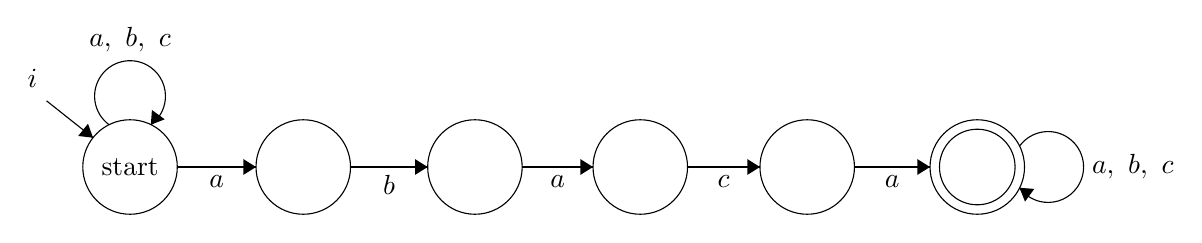
\begin{tikzpicture}[scale=0.2]
						\tikzstyle{every node}+=[inner sep=0pt]
						\draw [black] (11.3,-16.7) circle (3);
						\draw (11.3,-16.7) node {start};
						\draw [black] (22.3,-16.7) circle (3);
						\draw [black] (33.2,-16.7) circle (3);
						\draw [black] (43.7,-16.7) circle (3);
						\draw [black] (54.3,-16.7) circle (3);
						\draw [black] (65.1,-16.7) circle (3);
						\draw [black] (65.1,-16.7) circle (2.4);
						\draw [black] (6,-12.5) -- (8.95,-14.84);
						\draw (5.44,-11.08) node [left] {$i$};
						\fill [black] (8.95,-14.84) -- (8.63,-13.95) -- (8.01,-14.73);
						\draw [black] (9.977,-14.02) arc (234:-54:2.25);
						\draw (11.3,-9.45) node [above] {$a,\mbox{ }b,\mbox{ }c$};
						\fill [black] (12.62,-14.02) -- (13.5,-13.67) -- (12.69,-13.08);
						\draw [black] (67.78,-15.377) arc (144:-144:2.25);
						\draw (72.35,-16.7) node [right] {$a,\mbox{ }b,\mbox{ }c$};
						\fill [black] (67.78,-18.02) -- (68.13,-18.9) -- (68.72,-18.09);
						\draw [black] (14.3,-16.7) -- (19.3,-16.7);
						\fill [black] (19.3,-16.7) -- (18.5,-16.2) -- (18.5,-17.2);
						\draw (16.8,-17.2) node [below] {$a$};
						\draw [black] (25.3,-16.7) -- (30.2,-16.7);
						\fill [black] (30.2,-16.7) -- (29.4,-16.2) -- (29.4,-17.2);
						\draw (27.75,-17.2) node [below] {$b$};
						\draw [black] (36.2,-16.7) -- (40.7,-16.7);
						\fill [black] (40.7,-16.7) -- (39.9,-16.2) -- (39.9,-17.2);
						\draw (38.45,-17.2) node [below] {$a$};
						\draw [black] (46.7,-16.7) -- (51.3,-16.7);
						\fill [black] (51.3,-16.7) -- (50.5,-16.2) -- (50.5,-17.2);
						\draw (49,-17.2) node [below] {$c$};
						\draw [black] (57.3,-16.7) -- (62.1,-16.7);
						\fill [black] (62.1,-16.7) -- (61.3,-16.2) -- (61.3,-17.2);
						\draw (59.7,-17.2) node [below] {$a$};
					\end{tikzpicture}
				\end{center}
			\end{ex}
		\subsection{Regular Expressions} \lecture{February 15, 2013}
			Regular expressions are a textual notation to specify regular languages, based on a generative definition. Every regular expression can be translated into an $\epsilon$-NFA. Any regular language can be expressed as a regular expression, but it's not always simple. However, it's a more intuitive way to express a language in typed form than using a typed bubble diagram.

			\begin{center}
				\begin{tabular}{c|c|c}
					Regular Expression $R$ & Language $L(R)$ & Comments / Examples \\ \hline
					$a$ & $\set{a}$ & $a \in \Sigma$ \\
					$\epsilon$ & $\set{\epsilon}$ &  NULL string \\
					$R_1 R_2$ & $L(R_1) L(R_2)$ & Concatenation. e.g.:  \\
					& & $L(ab) = \set{ab}$ \\
					& & $L(abc) = \set{abc}$ \\
					& & $L(\epsilon a) = \set{a}$ \\
					$R_1 | R_2$ & $L(R_1) \cup L(R_2)$ & e.g. $L(abc | def) = \set{abc, def}$ \\
					$R \star$ & $L(R)^\star$ & Kleene closure. e.g.: \\
					& & $(abc) \star = \set{\epsilon, abc, abcabc, \ldots}$ \\
					$\emptyset$ & $\set{}$ & Empty language.
				\end{tabular}
			\end{center}

			\begin{ex}
				Given the alphabet $\Sigma = \set{0, 1}$, we're interested in the language $L(R)$ of all binary integers. The regular expression $R$ would be defined as $R = 0 | 1(0 | 1)^\star$.
			\end{ex}

			\begin{ex}
				Given the alphabet $\Sigma = \set{a, b}$, we're interested in the language $L(R)$ of all strings with an even number of $a$'s. Note that $L = \set{\epsilon, babbab, \ldots}$. We could define the regular expression for this language in several different ways:
				\begin{align*}
					R &= (b^\star{} ab^\star{} ab^\star{})^\star \\
					&= b^\star{}(b^\star{}ab^\star{}ab^\star{})^\star \\
					&= b^\star{}(ab^\star{}ab^\star{})^\star \\
					&= (b^\star{}ab^\star{}a)b^\star \\
					&= b^\star{}(b^\star{}ab^\star{}ab^\star{})^\star{} b^\star \\
					&\vdots
				\end{align*}

				This illustrates an important point: there are many ways to express any particular regular language with regular expressions. There is not necessarily a unique minimal regular expression for a language. Also, we don't care if the regular expression is ambiguous or not.
			\end{ex}

			\begin{ex}
				Let $\Sigma = \set{0, 1, +}$, and $L(R)$ be the sum of one or more integers. We can express this as the regular expression $R$:
				\begin{align*}
					R &= 0 | 1 (0 | 1)^\star{} (+ 0|1(0|1)^\star{})^\star
				\end{align*}

				Note that + is an extended regular expression, but we'll assume it isn't for now. We'll talk more about that shortly.
			\end{ex}

			\begin{ex}
				Let $\Sigma = \set{0, 1, +}$ (as before), but now let $L(R)$ be the sum of two or more integers. We can express this as the regular expression $R$:
				\begin{align*}
					R = 0|1(0|1)^\star{} + 0|1(0|1)^\star{} (+ 0|1(0|1)^\star{})^\star
				\end{align*}

				As you can see, this becomes tedious. There are some regular expressions that grow exponentially as you make minor changes like these.
			\end{ex}

			\subsubsection{Extensions}
				Extensions give a more terse (sometimes exponentially) notation but they still only specify the regular languages.

				\begin{center}
					\begin{tabular}{c|c}
						Extended RE & Meaning \\ \hline
						$R^+$ & $RR^\star$ \\
						$\set{R_1 \text{\textbf{|}} R_2}$ & $R_1(R_2R_1)^\star$ \\
						$\set{R_1 \text{\textbf{||}} R_2}$ & $R_1(R_2R_1)^+$
					\end{tabular}
				\end{center}
				(the vertical bars in the above table are fatter than normal)
				\\ \\
				The $R^+$ case is where we would see an exponential increase in notation if we weren't using extensions, if there were nested expressions containing +.
				\\ \\
				We could have expressed the earlier expression as $\set{0|1(0|1)^\star{} \text{\textbf{|}} +}$.
				\\ \\
				In practice, many people call regexps ``regular expressions,'' but they aren't true regular expressions because they can express more than just the regular languages. When \emph{we} say ``regular expressions,'' we really mean true regular expressions (expressions that can only represent regular languages).

			\subsubsection{Regular Expressions to Finite Automata}
				Any regular expression can be converted to an $\epsilon$-NFA that recognizes the language. In fact, an $\epsilon$-NFA for a regular expression will always have exactly one final state. In addition, recall that any $\epsilon$-NFA can be converted to a DFA using subset construction.
				\\ \\
				If you have the regular expression $a$, or a regular expression $\epsilon$, we can express that as an $\epsilon$-NFA by creating a start state that is joined to the final state by either $a$ or $\epsilon$, respectively.
				\\ \\
				If we have a regular expression $R_1 R_2$ (where $R_1$ and $R_2$ are also regular expressions), we will have $\epsilon$-NFAs for $R_1$ and $R_2$ already. We simply make the final state from $R_1$ no longer a final state, and connect it with $\epsilon$ to the start state of $R_2$.
				\\ \\
				If we have a regular expression $R_1 | R_2$ (where $R_1$ and $R_2$ are also regular expressions), we will have $\epsilon$-NFAs for $R_1$ and $R_2$ already. We create a new final state, and we make the final states of $R_1$ and $R_2$ connected to the new final state through $\epsilon$. The final states of $R_1$ and $R_2$ are no longer final states themselves. We also create a new start state that connects to the start states of both $R_1$ and $R_2$ through $\epsilon$.
				\\ \\
				If we have a regular expression $R^\star$ (where $R$ is a regular expression), we will have an $\epsilon$-NFA for $R$ already. We add a new start state and a new final state, and make the final state of $R$ no longer a final state. We connect the new start state to both the start state of $R$ and the new final state, both through $\epsilon$. The previously-final state of $R$ is also connected to the new final state through $\epsilon$.
				\\ \\
				If we have $\emptyset$, we create a start state and a final state and provide no path between the two.

	\section{Context-Free Languages} \lecture{February 25, 2013}
		Context-free languages (CFLs) are a larger class of languages than regular languages. They capture recursion through matching brackets (\verb+([()])+) and nesting structures (\verb+if then if then else else+).
		\\ \\
		Every regular language is also a context-free language, however there are context-free languages that are not regular languages. Context-free languages that are not regular would be languages that require an infinite number of states in order to be expressed as a state machine. However, all regular languages can be expressed in a \underline{finite} state machine, so those languages with an infinite number of states cannot be regular.
		\begin{ex}
			An example of a context-free language that is not regular is the language defined by:
			\begin{align*}
				\Sigma &= \set{(, )} \\
				L &= \set{\epsilon, (), (()), ((())), \ldots}
			\end{align*}

			That is, $L$ is the language of all strings containing $n$ opening parentheses and $n$ (matching) closing parentheses.
		\end{ex}

		\begin{defn}
			There are two definitions of \textbf{context-free languages}. A context-free language is:
			\begin{itemize}
				\item Any language generated by a context-free grammar.
				\item Any language recognized by a (nondeterministic) pushdown automaton (PDA).
			\end{itemize}
		\end{defn}

		\begin{defn}
			A \textbf{pushdown automaton} (PDA) is a machine with finite memory and an unbounded (infinite) stack.
		\end{defn}

		A pushdown automaton could be used to match parentheses and do similar recursive operations because it has an infinite stack.
		\\ \\
		Notice how a context-free language needs to be recognized by a \underline{nondeterministic} pushdown automaton. The best running time of a pushdown automaton is approximately $O(n^{2.73}) \approx O(n^3)$ in the real world. This complexity makes nondeterministic pushdown automata only useful when we are dealing with small strings.
		\\ \\
		Some context-free languages can be recognized by a deterministic pushdown automaton (DPDA). This can be achieved in $O(n)$ time. These context-free languages are called \textbf{deterministic context-free languages}.

		\subsection{Context-Free Grammars}
			A context-free grammar (CTG) consists of:
			\begin{itemize}
				\item $T$: a finite set of terminal symbols (terminals), sometimes referred to as the alphabet $\Sigma$.
				\item $N$: a finite set of non-terminal symbols (nonterminals), sometimes referred to as variables.
				\item $S \in N$: a start symbol.
				\item $R$: a set of rules. $R = \set{A \to \alpha | A \in N, \alpha \in (N \cup T)^\star}$
			\end{itemize}

			\textbf{Notation} (by convention only):
			\begin{itemize}
				\item $a, b, c, d$ are terminal symbols.
				\item $A, B, C, D$ are nonterminal symbols.
				\item $V$ is the vocabulary $V = N \cup T$.
				\item $w, x, y, z$ are strings of terminals.
				\item $\alpha, \beta, \gamma, \delta$ are strings of vocabulary symbols (terminals and/or nonterminals).
			\end{itemize}

			\begin{ex}
				We have the context-free grammar $G$, where $R$ is defined as:
				\begin{align*}
					S &\to AhB \\
					A &\to ab \\
					A &\to cd \\
					B &\to ef \\
					B &\to g
				\end{align*}

				We also have $T = \set{a, b, c, d, e, f, g, h}, N = \set{S, A, B}$, and $S = S$. We usually just write $R$ and the rest of the components of the grammar can be inferred. The language generated by $G$ is a finite (and regular) language $L(G) = \set{abhef, abhg, cdhef, cdhg}$.

				\begin{align*}
					\gamma_0&: &\implies& S \\
					\gamma_1&: S \mapsto AhB &\implies& AhB \\
					\gamma_2&: A \mapsto cd &\implies& cdhB \\
					\gamma_3&: B \mapsto g &\implies& cdhg
				\end{align*}
				This is called a \textbf{derivation}.
			\end{ex}

			\begin{defn}
				$\alpha A \beta \implies \alpha \gamma \beta$. $\implies$ here roughly means ``derives in one step.'' More precisely, $A \to \gamma \in R$.
			\end{defn}

			\begin{defn}
				$\alpha \stackrel{\star}{\implies} \beta$. $\stackrel{\star}{\implies}$ here roughly means ``derives in zero or more steps.'' More precisely, it means either $\alpha = \beta$ \emph{or} $\exists \gamma . \alpha \implies \gamma$ and $\gamma \stackrel{\star}{\implies} \beta$.
				\\ \\
				$\stackrel{\star}{\implies}$ is the reflexive, transitive closure of $\implies$.
			\end{defn}

			\begin{defn}
				A \textbf{derivation} of some string $x$ with respect to some context-free grammar $G$ is the sequence $\gamma_0, \gamma_1, \gamma_2, \ldots, \gamma_n$ where:
				\begin{align*}
					\gamma_0 &= S \\
					\gamma_n &= x \\
					\gamma_i &\implies \gamma_{i + 1} \text{ for } 0 \le i < n
				\end{align*}
			\end{defn}

			We could express $L(G)$ as $L(G) = \set{x | S \stackrel{\star}{\implies} x}$.

			\begin{defn}
				$x$ is a sequence of terminals. $x$ is sometimes called a \textbf{member} in $L(G)$, a \textbf{word} in $L(G)$, or a \textbf{sentence} in $L(G)$. All of this terminology means the same thing.
			\end{defn}

			\begin{defn}
				$\gamma_i$ where $S \stackrel{\star}{\implies} \gamma_i$ is called a \textbf{derivation step} or a \textbf{sentential form}.
			\end{defn}

		\subsection{Parsing}
			Given some $x \in L(G)$, find a derivation for $x$. Parsing and recognition is when if $x \in L(G)$, you find a derivation, otherwise you reject. It's your duty to reject $x \not \in L(G)$, but it'd be nice if you could also be somewhat informative as to why $x \not \in L(G)$.
			\\ \\
			There are two general approaches for parsing: top-down and bottom-up.
			\subsubsection{Top-Down Parsing}
				Top-down parsing is where you start with $\gamma_0 = S$ and continue until you find $\gamma_n = x$. Our example from earlier was an example of this:
				\begin{align*}
					\gamma_0&: &\implies& S \\
					\gamma_1&: S \mapsto AhB &\implies& AhB \\
					\gamma_2&: A \mapsto cd &\implies& cdhB \\
					\gamma_3&: B \mapsto g &\implies& cdhg
				\end{align*}
				This is a \textbf{leftmost derivation}.

			\subsubsection{Bottom-Up Parsing}
				Bottom-up parsing is where you start with $\gamma_n = x$ and continue until you find $\gamma_0 = S$. Here's an example of a bottom-up parse:
				\begin{align*}
					\gamma_n&: &\implies& cdhg \\
					\gamma_{n - 1}&: cd \mapsto A &\implies& Ahg \\
					\gamma_{n - 2}&: g \mapsto B &\implies& AhB \\
					\gamma_{n - 3}&: AhB \mapsto S &\implies& S
				\end{align*}

				This is a \textbf{rightmost derivation}.
				\\ \\
				By convention, we will rewrite this derivation in reverse order:
				\begin{align*}
					\gamma_0&: &\implies& S \\
					\gamma_1&: S \mapsto AhB &\implies& AhB \\
					\gamma_2&: B \mapsto g &\implies& Ahg \\
					\gamma_3&: A \mapsto cd &\implies& cdhg
				\end{align*}

				Note that the $\gamma_2$ for these two parsing examples is different. This is because we used leftmost derivation for the top-down example and rightmost derivation for the bottom-up example. Leftmost and rightmost derivations are \textbf{canonical forms}, since there are many other arbitrary decisions we could have made for the order of our derivation steps.
				\begin{defn}
					A \textbf{leftmost derivation} replaces the leftmost nonterminal first. A \textbf{rightmost derivation} replaces the rightmost nonterminal first.
				\end{defn}

				Note that in the bottom-up example, we still appear to have replaced the leftmost nonterminal first, but since the order of our steps gets reversed, it seems like we performed a rightmost derivation instead.
			\subsubsection{Parse Trees}
				A parse tree is another canonical parsing form. You can draw a tree to represent the string:
				\begin{figure}[h]
					\Tree [.S [.A [.c ] [.d ] ] [.h ] [.B [.g ] ] ]
				\end{figure}

				Using a parse tree has the advantage of not having to rewrite the entire sentential form at each derivation step. It's also easier to visually traverse what has changed at each step.
				\\ \\
				Parse trees remove irrelevant differences, however we could still have some ambiguity as with the other parsing methods. Ambiguity is acceptable for context-free grammars, but it's sometimes easier to make compilers that deal with unambiguous grammars.
		\subsection{Parsing WLPP} \lecture{February 27, 2013}
			WLPP is described in lexical syntax (splitting WLPP source into tokens), context-free syntax (how to arrange the tokens to create a valid WLPP program), and context-sensitive syntax (other rules that cannot be expressed by a context-free grammar).
			\\ \\
			The start symbol is always \verb+procedure+. We parse the tokens in order. When we encounter a nonterminal symbol, we look for a rule that defines it (on the following lines). We perform a substitution based on the rule we found, and then check the continual validity of token kinds in that order.
			\\ \\
			Note that declarations can be defined recursively in these grammars.
			\\ \\
			For more information, see the \href{https://www.student.cs.uwaterloo.ca/~cs241/wlpp/WLPP.html}{WLPP specification}.
		\subsection{Some Parsing Examples}
			\begin{ex}
				We're given the alphabet $\Sigma = \set{a, b}$, the language $L = \set{\epsilon, a, aa, aaa, \ldots}$ (that is, $a^\star$), and the following rules $R$:
				\begin{align*}
					S &\to \epsilon \\
					S &\to Sa
				\end{align*}

				Let's derive $x = aaa$ using a parse tree.
				\begin{figure}[H]
					\Tree [.S [.S [.S [.S [.$\epsilon$ ] ] [.a ] ] [.a ] ] [.a ] ]
				\end{figure}

				This could also be expressed as a derivation like so:
				\begin{align*}
					&S \\
					&Sa \\
					&Saa \\
					&Saaa \\
					&aaa
				\end{align*}

				That derivation is both a leftmost and rightmost derivation. This grammar is called \textbf{left-recursive} or \textbf{left-associative}.
			\end{ex}

			\begin{ex}
				Given the same alphabet and language as before, we could have also had this set of rules $R$:
				\begin{align*}
					S &\to \epsilon \\
					S &\to aS
				\end{align*}

				Let's again look at deriving $x = aaa$, but with these new rules.
				\begin{figure}[H]
					\Tree [.S [.a ] [.S [.a ] [.S [.a ] [.S [.$\epsilon$ ] ] ] ] ]
				\end{figure}

				This could also be expressed as a derivation like so:
				\begin{align*}
					S& \\
					aS& \\
					aaS& \\
					aaaS& \\
					aaa&
				\end{align*}

				This grammar is called \textbf{right-recursive} or \textbf{right-associative}.
			\end{ex}

			\begin{ex}
				Given the same alphabet and language as before, we could have also had this set of rules $R$:
				\begin{align*}
					S &\to \epsilon \\
					S &\to a \\
					S &\to SS
				\end{align*}

				Let's again look at deriving $x = aaa$, but with these new rules.
				\begin{figure}[H]
					\Tree [.S [.S [.S [.a ] ] [.S [.a ]]] [.S [.a ] ] ]
					\Tree [.S [.S [.a ] ] [.S [.S [.a ] ] [.S [.a ] ] ] ]
				\end{figure}

				We have two different parse trees, which means this grammar is ambiguous. That is, there are two canonical forms.
				\\ \\
				We have two different leftmost derivations for $x = aaa$. The first leftmost derivation is:
				\begin{align*}
					&S \\
					&SS \\
					&SSS \\
					&aSS \\
					&aaa
				\end{align*}

				The second leftmost derivation is:
				\begin{align*}
					&S \\
					&SS \\
					&aS \\
					&aSS \\
					&aaS \\
					& aaa
				\end{align*}

				Note that these two derivations are different.
				\\ \\
				Similarly, there are two different rightmost derivations. The first rightmost derivation is:
				\begin{align*}
					S& \\
					SS& \\
					Sa& \\
					SSa& \\
					Saa& \\
					aaa
				\end{align*}

				The second rightmost derivation is:
				\begin{align*}
					S& \\
					SS& \\
					SSS& \\
					SSa& \\
					Saa& \\
					aaa
				\end{align*}

				Once again, note that these two derivations are different.
			\end{ex}

			\begin{ex}
				Assume the context-free grammar as specified in the \href{https://www.student.cs.uwaterloo.ca/~cs241/wlpp/WLPP.html}{WLPP specification}.
				\\ \\
				Let's parse \verb+int* x = 25;+. We get the following parse tree:
				\begin{figure}[H]
					\Tree [.dcls [.dcls [.$\epsilon$ ] ] [.dcl [.INT ] [.STAR ] [.ID ] ] [.BECOMES ] [.NUM ] [.SEMI ] ]
				\end{figure}

				Technically, this shouldn't be valid, because type \verb+int*+ cannot be assigned the value 25. However, this context-free grammar does not enforce that \textendash{} the context-sensitive syntax will. It was decided that this grammar was sufficient to construct a parse tree, although if we wanted we could enforce that constrain in a context-free grammar.
				\\ \\
				It is sometimes the case that adding seemingly-simple constraints like these will make the grammar quite complicated, so it's sometimes better to just leave certain restrictions for enforcement through a context-sensitive syntax instead.
			\end{ex}

		\subsection{Formalizing Derivations}
			We'll start off with two formal definitions for leftmost derivations.

			\begin{defn}
				$xA\beta \implies x \gamma \beta := A \to \gamma \in R$. That is, you must substitute the first nonterminal symbol.
			\end{defn}

			\begin{defn}
				$\alpha \stackrel{\star}{\implies} \beta := \alpha = \beta \text{ OR } \exists \gamma \cdot \alpha \implies \gamma, \gamma \stackrel{\star}{\implies} \beta$.
			\end{defn}

			We have similar definitions for rightmost derivations, as follows.

			\begin{defn}
				$\alpha Ay \implies \alpha \gamma y := A \to \gamma \in R$.
			\end{defn}

			\begin{defn}
				$\alpha \stackrel{\star}{\implies} \beta := \alpha = \beta \text{ OR } \exists \gamma \cdot \alpha \implies \gamma, \gamma \stackrel{\star}{\implies} \beta$.
			\end{defn}

			We will now formally define ambiguity in a context-free grammar.

			\begin{defn}
				A grammar $G$ is \textbf{ambiguous} if there exists $x \in L(G)$ such that:
				\begin{itemize}
					\item There are two or more leftmost derivations for $x$, or equivalently,
					\item There are two or more rightmost derivations for $x$, or equivalently,
					\item There are two or more parse trees for $x$.
				\end{itemize}
			\end{defn}

			Often, there is a different grammar $G'$ where $L(G') = L(G)$ and $G'$ is unambiguous. But, $G'$ may not be easy to find, or $G'$ may not exist at all. If $G'$ does not exist, we say $L(G)$ is \textbf{inherently ambiguous}.
			\\ \\
			We're interested in unambiguous grammars because they allow us to do syntax-directed translation.
		\subsection{Syntax-Directed Translation}
			Syntax-directed translation involves computing the ``meaning'' for all subtrees in the parse.

			\begin{ex}
				Let $T = \set{0, 1}, N = \set{I, B}, S = I$, and $R$ be the set of rules:
				\begin{align*}
					I &\to 0 \\
					I &\to B \\
					B &\to 1 \\
					B &\to B0 \\
					B &\to B1
				\end{align*}

				We're interested in the language of binary integers without leading zeros, that is, $\set{0, 1, 10, 11, 100, 101, \ldots}$.
				\\ \\
				Let's parse the big-endian value of $x = 110$. We have the parse tree:
				\begin{figure}[H]
					\Tree [.I [.B [.B [.B [.1 ] ] [.1 ] ] [.0 ] ] ]
				\end{figure}

				From the bottom of the tree, the meaning of $B$ is 1. The meaning of the next $B$ is 3, since $\text{Meaning}(B) = 2 \times 1 + 1$. The meaning of the uppermost $B$, and $I$, are 6. The meaning of a particular element is determined by its subtrees.
				\\ \\
				Suppose instead we wanted the little-endian binary unsigned value. That's reasonably difficult with this grammar. Instead, we'll use a right-associative grammar for the same language. Let's define the rules for this new grammar to be:
				\begin{align*}
					I &\to 0 \\
					I &\to B \\
					B &\to 1 \\
					B &\to 0B \\
					B &\to 1B \\
					B &\to 0
				\end{align*}

				Actually, this example is broken, since the number $110$ has a useless leading zero when interpreted as a little-endian binary value. So, we added the last rule, $B \to 0$ to allow leading zeroes.
				\\ \\
				We have the following parse tree:
				\begin{figure}[H]
					\Tree [.I [.B [.1 ] [.B [.1 ] [.B [.0 ] ] ] ] ]
				\end{figure}

				From the bottom of the tree, the meaning of $B$ is 0, the meaning of the second $B$ is 1, and the meaning of the uppermost $B$ (and $I$) is 3.
			\end{ex}

			\begin{ex} \lecture{March 1, 2013}
				Let's change the rules $R$, to be:
				\begin{align*}
					I &\to 0 \\
					I &\to B \\
					I &\to 1 \\
					I &\to B0 \\
					I &\to B1
				\end{align*}

				We're interested in the meaning of $x = 1101 \in L(G)$ as a binary big-endian number. $x$ means 13 in big-endian. We get this parse tree:
				\begin{figure}[H]
					\Tree [.I [.B [.B [.B [.1 ] [.1 ] ] [.0 ] ] [.1 ] ] ]
				\end{figure}


				The meaning of an individual node is called its \textbf{attribute}. The attribute of the lowest $B$ is 3, then 6, then 13. We denote the attribute of $I$ as $m(I) = 13$. To determine the meaning, you determine the meaning of the subtrees first by doing a postfix traversal.
				\\ \\
				What about the little-endian meaning? The best way to determine this is to write another grammar that is right-associative. We'll define the rules $R$ as:
				\begin{align*}
					I &\to 0 \\
					I &\to B \\
					B &\to 1 \\
					B &\to 0B \\
					B &\to 1B
				\end{align*}

				This is the parse tree for $x = 1101$ as a little-endian binary number:
				\begin{figure}[H]
					\Tree [.I [.B [.1 ] [.B [.1 ] [.B [.0 ] [.B [.1 ] ] ] ] ] ]
				\end{figure}
			\end{ex}
		\subsection{Extended Grammars}
			Let's extend the grammar from before to add these rules to $R$:
			\begin{align*}
				E &\to I \\
				E &\to E + I
			\end{align*}

			Now, let's parse \verb|1 + 1 + 0|. We get the parse tree:
			\begin{figure}[H]
				\Tree [.E [.E [.E [.I [.B [.1 ] ] ] ] [.+ ] [.I [.B [.1 ] ] ] ] [.+ ] [.I [.0 ] ] ]
			\end{figure}

			The meaning of the $E + I$ expression at the second level is $m(E) = 2$ and $m(I) = 0$, so the resulting meaning for the uppermost $E$ is $m(E) = 2$.
			\\ \\
			Now, let's extend the grammar once more to include these rules for $E$, in addition to the rules for $I$ that were defined earlier:
			\begin{align*}
				E &\to I \\
				E &\to E + I \\
				E &\to E * I
			\end{align*}

			Now, let's try to parse \verb|1 + 1 * 0|. We get the parse tree:
			\begin{figure}[H]
				\Tree [.E [.E [.E [.I [.B [.0 ] ] ] ] [.+ ] [.I [.B [.1 ] ] ] ] [.* ] [.I [.0 ] ] ]
			\end{figure}

			If you examine the attributes, you'll see that the uppermost \verb|E * I| expression has $m(E) = 2$ and $m(I) = 0$, which gives the attribute of the uppermost $E$ to be $m(E) = 0$. This is mathematically incorrect.
			\\ \\
			To get around this, we'll introduce the notion of a term $T$. We'll re-define the rules for $E$ once more:
			\begin{align*}
				E &\to T \\
				E &\to E + T \\
				T &\to I \\
				T &\to T * I
			\end{align*}

			Now, when we parse \verb|1 + 1 * 0|, we get this parse tree:
			\begin{figure}[H]
				\Tree [.E [.E [.T [.I [.B [.1 ] ] ] ] ] [.+ ] [.T [.T [.I [.B [.1 ] ] ] ] [.* ] [.I [.B [.0 ] ] ] ] ]
			\end{figure}

			This yields the proper values for the uppermost \verb|E + T| expression, $m(E) = 1$ and $m(T) = 0$. This works as we would mathematically expect.
			\\ \\
			You can see this general pattern of evaluation ordering in the WLPP spec, but instead of $I$ and $B$, we will have specific INT tokens. Here's an example of a WLPP parse tree, parsing \verb|1 + 1 * 0|.
			\begin{figure}[H]
				\Tree [.E [.E [.T [.{INT 1} ] ] ] [.+ ] [.T [.T [.{INT 1} ] ] [.* ] [.{INT 0} ] ] ]
			\end{figure}
		\subsection{Parsing Algorithms}
			There are several different parsing algorithms, some of which are top-down and some of which are bottom-up.
			\subsubsection{Generic Top-Down Parser}
				Given $x \in L(G)$, find a derivation $\gamma_0 \gamma_1 \ldots \gamma_n$.

				\begin{algorithm}[H]
					$\gamma = S$\;
					\While{$\gamma \ne x$}{
						select $\alpha, A, \beta$ where $\gamma = \alpha A \beta$ (find a nonterminal $A$ in $\gamma$)\;
						select $\delta$ where $A \to \delta \in R$ (find a rule with $A$ as its left side, may fail if $x \not \in L(G)$)\;
						$\gamma = \alpha \delta \beta$\;
					}
				\end{algorithm}

				\begin{ex}
					We're given the following set of rules $R$:
					\begin{align*}
						S &\to AhB \\
						A &\to ab \\
						B &\to ef \\
						B &\to g
					\end{align*}

					Let's parse $x = abhg$. We get:
					\begin{align*}
						\gamma &= S, A = S, \alpha = \beta = \epsilon, \delta = AhB \\
						\gamma &= AhB, A = A \text{ (or } A = B), \alpha = \epsilon, \beta = hB, \delta = ab \text{ by oracle} \\
						\gamma &= abhB \\
						\gamma &= abhg
					\end{align*}
				\end{ex}

			\subsubsection{Stack-Based Top-Down Parser}
				Given input $x = x_0 x_1 x_2 \ldots x_{|x|-1}$, we'll read $x$ from left to right. At any step, we have:
				\begin{align*}
					x = \underbrace{x_0 x_1 x_2}_{\text{input read so far}} \ldots \underbrace{x_i x_{i + 1} \ldots x_{|x| - 1}}_{\text{input yet to be read}}
				\end{align*}

				We also have a stack of vocabulary symbols:
				\begin{align*}
					\text{stack} = X_0X_1 \ldots X_{|\text{stack}|-1}
				\end{align*}

				where $X_0$ is the top of the stack and $X_{|\text{stack}|-1}$ is the bottom of the stack.
				\\ \\
				A key observation: at all steps, we have:
				\begin{align*}
					\gamma = (\text{input read so far}) (\text{stack})
				\end{align*}

				\begin{ex}
					Let's parse $x = abhg$.
					\begin{center}
						\begin{tabular}{|c|c|c|c|}
							\hline
							$\gamma$ & input read & input yet to be read & stack (top $\ldots$ bottom) \\ \hline
							S & $\epsilon$ & abhg & S \\
							AhB & $\epsilon$ & abhg & AhB \\
							abhB & $\epsilon$ & abhg & abhB \\
							abhB & a & bhg & bhB \\
							abhB & ab & hg & hB \\
							abhB & abh & g & B \\
							abh & abh & g & g \\
							abhg & abhg & $\epsilon$ & $\epsilon$ \\ \hline
						\end{tabular}
					\end{center}

					We're popping a terminal from the stack and comparing it with the input. When both the input to be read and the stack are empty, we're done.
				\end{ex}

				Here's some pseudocode for a stack-based top-down parser:

				\begin{algorithm}[H]
					push $S$ onto stack\;
					\For{$c = x_0, x_1, x_2, \ldots, x_{|x| - 1}$}{
						\While{top of stack is $A \in N$}{
							consult oracle to determine $\delta$ where $A \to \delta \in R$\;
							pop stack\;
							push $\delta_{|\delta|-1}$\;
							push $\delta_{|\delta|-2}$\;
							$\vdots$ \\
							push $\delta_0$\;
						}
						assert $c = \text{top of stack}$\;
						pop stack\;
					}
					assert stack = $\epsilon$\;
				\end{algorithm}

				\lecture{March 4, 2013}
				The crux of a stack-based top-down parser is in each derivation step, we have this invariant:
				\begin{align*}
					\gamma &= (\text{input read so far}) (\text{stack: top \ldots bottom})
				\end{align*}

			\subsubsection{LL(1) Parsing}
				The name ``LL(1)'' comes from the fact that this parsing algorithm reads input from left-to-right, and it uses leftmost derivations. An oracle uses one symbol of lookahead \textendash{} that is, it looks at $A$ (the nonterminal to expand) and $c$ (the next input symbol) in order to choose $A \to \alpha \in R$.
				\\ \\
				The oracle is represented as a Predict function, Predict: $N \times T \to 2^R$ (that is, it yields a subset of the set of rules $R$).
				\\ \\
				As a convenience, we'll introduce the notion of an augmented grammar.
				\begin{defn}
					Given $G$, the \textbf{augmented grammar} $G'$ is:
					\begin{align*}
						N' &= N \cup \set{S'} \text{ where } S' \text{ is the new start symbol} \\
						S' &= S' \\
						T' &= T \cup \set{\vdash, \dashv} \text{ where } \vdash \text{ and } \dashv \text{ are the beginning and end string markers} \\
						R' &= R \cup \set{S' \to{} \vdash S \dashv}
					\end{align*}
				\end{defn}

				Let's introduce a specific augmented grammar with the following set of rules $R'$:
				\setcounter{equation}{0}
				\begin{align}
					S' &\to{} \vdash S \dashv \\
					S &\to AhB \\
					A &\to ab \\
					A &\to cd \\
					B &\to ef \\
					B &\to g
				\end{align}

				A derivation for some input $x$ would look like:
				\begin{align*}
					\gamma_0 &={} \vdash S' \dashv \\
					\vdots& \\
					\gamma_n &={} \vdash x \dashv
				\end{align*}

				Let's get back to our Predict function. We have the following table which represents the logic the oracle uses:
				\begin{center}
					\begin{tabular}{|c|c|c|c|c|c|c|c|c|c|c|}
						\hline
						& \textbf{a} & \textbf{b} & \textbf{c} & \textbf{d} & \textbf{e} & \textbf{f} & \textbf{g} & \textbf{h} & $\boldsymbol \vdash$ & $\boldsymbol \dashv$ \\ \hline
						\textbf{S'} & $\set{}$ & $\set{}$ & $\set{}$ & $\set{}$ & $\set{}$ & $\set{}$ & $\set{}$ & $\set{}$ & $\set{1}$ & $\set{}$ \\
						\textbf{S} & $\set{2}$ & $\set{}$ & $\set{2}$ & $\set{}$ & $\set{}$ & $\set{}$ & $\set{}$ & $\set{}$ & $\set{}$ & $\set{}$ \\
						\textbf{A} & $\set{3}$ & $\set{}$ & $\set{4}$ & $\set{}$ & $\set{}$ & $\set{}$ & $\set{}$ & $\set{}$ & $\set{}$ & $\set{}$ \\
						\textbf{B} & $\set{}$ & $\set{}$ & $\set{}$ & $\set{}$ & $\set{5}$ & $\set{}$ & $\set{6}$ & $\set{}$ & $\set{}$ & $\set{}$ \\ \hline
					\end{tabular}
				\end{center}

				The $(B, e)$ position in this table means if $e$ is the next symbol, rule 5 must be used. We could have drawn this table without empty sets all over the place \textendash{} blank spaces indicate empty sets of applicable rules.
				\\ \\
				Here's the pseudocode for an LL(1) parser for input $x$: \\
				\begin{algorithm}[H]
					push $\dashv$\;
					push $S$\;
					push $\vdash$\;
					\For{c in $\vdash x \dashv$}{
						\While{top of stack is some $A \in N$}{
							assert Predict$[A, c]$ = $\set{A \to X_0 X_1 \ldots X_m}$\;
							pop stack\;
							push $X_m$\;
							push $X_{m - 1}$\;
							$\vdots$ \\
							push $X_0$;
						}
						assert top of stack = $c$\;
						pop stack;
					}
					assert stack = $\epsilon$;
				\end{algorithm}

				\underline{Aside}: if we added the rule (7) $A \to abdc$, we would have a set of two elements for $[A, a]$, which means the grammar would no longer be an LL(1) grammar. LL(1) is a deterministic parser. If we wanted to support multiple rules, like by adding that rule (7), we could build a non-LL(1) nondeterministic parser.
				\\ \\
				Here's a sample LL(1) parse:
				\begin{center}
					\begin{tabular}{|c|c|c|c|c|}
						\hline
						$\gamma$ & input read & not read & stack (top \ldots bottom) & action \\ \hline
						$\vdash S \dashv$ & $\epsilon$ & $\vdash abhg \dashv$ & $\vdash S \dashv$ & assert $\vdash = \vdash$ \\
						$\vdash S \dashv$ & $\vdash$ & $abhg \dashv$ & $S \dashv$ & read $\vdash$ \\
						$\vdash AhB \dashv$ & $\vdash$ & $abhg \dashv$ & $AhB \dashv$ & Predict[S, a] = $\set{S \to AhB}$ \\
						$\vdash abhB \dashv$ & $\vdash$ & $abhg \dashv$ & $abhB \dashv$ & Predict[A, a] = $\set{A \to ab}$ \\
						$\vdash abhB \dashv$ & $\vdash a$ & $bhg \dashv$ & $bhB \dashv$ & assert $a = a$, read $a$ \\
						$\vdash abhB \dashv$ & $\vdash ab$ & $hg \dashv$ & $hB \dashv$ & assert $b = b$, read $b$ \\
						$\vdash abhB \dashv$ & $\vdash abh$ & $g \dashv$ & $B \dashv$ & assert $h = h$, read $h$ \\
						$\vdash abhg \dashv$ & $\vdash abh$ & $g \dashv$ & $g \dashv$ & Predict[B, g] = $\set{B \to g}$ \\
						$\vdash abhg \dashv$ & $\vdash abhg$ & $\dashv$ & $\dashv$ & assert $g = g$ \\
						$\vdash abhg \dashv$ & $\vdash abhg \dashv$ & $\epsilon$ & $\epsilon$ & assert stack = $\epsilon$ \\ \hline
					\end{tabular}
				\end{center}


				\textbf{Constructing the Predict Function}: we'll need some helper functions.
				\begin{itemize}
					\item first[$\alpha$] := $\set{a | \alpha \stackrel{\star}{\implies} a \beta}$. For example, first($A$) = $\set{a, c}$, and first($AbB$) = $\set{a}$.
					\item nullable[$\alpha$] := $\alpha \stackrel{\star}{\implies} \epsilon$.
					\item follow[$A$] := $\set{b | S' \stackrel{\star}{\implies} \alpha A b \beta}$. That is, in \emph{some} sentential form, $A$ is followed by these elements $b$.
				\end{itemize}

				Now, we can define Predict:
				\begin{align*}
					\text{Predict}[A, a] = \set{A \to \alpha \in R | a \in \text{first}(\alpha) \text{ OR } (\text{nullable}(\alpha) \text{ AND } a \in \text{follow}(A)}
				\end{align*}

				In the previous example, we didn't use the nullable rule because we did not have any rules leading to $\epsilon$.
				\\ \\
				\textbf{Observation}: if for all $A, a$, |Predict[$A$, $a$]| $\le$ 1, we say that $G$ is an LL(1) grammar. Otherwise, $G$ is not LL(1). We \emph{may} be able to write an LL(1) grammar for the same language.
				\begin{ex}
					Let $G$ be a grammar with the following set of rules $R$:
					\begin{align*}
						S' &\to{} \vdash S \dashv \\
						S &\to ab \\
						S &\to aab
					\end{align*}

					This grammar is not LL(1), because Predict[$S$, $a$] = $\set{S \to ab, S \to aab}$. In particular, |Predict[$A$, $a$]| $\not \le 1$ for all $A, a$.
					\\ \\
					We can fix this (and make it an LL(1) grammar) by changing $R$ to be the following set of rules:
					\begin{align*}
						S' &\to{} \vdash S \dashv \\
						S &\to aB \\
						B &\to b \\
						B &\to ab
					\end{align*}

					In this case, we have:
					\begin{align*}
						\text{Predict}[S, a] &= \set{S \to aB} \\
						\text{Predict}[B, a] &= \set{B \to ab} \\
						\text{Predict}[B, b] &= \set{B \to b}
					\end{align*}

					Now, |Predict[$A$, $a$]| $\le 1$ for all $A, a$, so this is an LL(1) grammar for the same language.
					\\ \\
					Similarly, we can find yet another LL(1) grammar for the same language. Let $R$ now be this set of rules:
					\begin{align*}
						S' &\to{} \vdash S \dashv \\
						S &\to aBb \\
						B &\to \\
						B &\to a
					\end{align*}

					Note that the third rule is $B$ mapping to nothing. That is, $B \to$ is nullable. We get these results from our Predict function:
					\begin{align*}
						\text{Predict}[S, a] &= \set{S \to aBb} \\
						\text{Predict}[B, a] &= \set{B \to a} \\
						\text{Predict}[B, b] &= \set{B \to}
					\end{align*}

					So, we have that $B \to $ is nullable and follow($B$) = $\set{b}$.
				\end{ex}

				If you use LL(1), you'll have to forget about left recursion, and therefore forget about syntax-directed translation as well. It doesn't work.
				\\ \\
				There are some languages for which no LL(1) grammar is possible.
				\begin{ex}
					Let's look at the language defined by the regular expression $a^\star(ab)^\star$. Here's a set of rules $R$ for that regular expression:
					\begin{align*}
						S &\to \epsilon \\
						S &\to aSb \\
						S &\to aaSb
					\end{align*}

					Note that this grammar is not LL(1) and it is ambiguous.
				\end{ex}

			\subsubsection{Stack-Based Bottom-Up Rightmost Parser} \lecture{March 6, 2013}
				\begin{ex}
					We're given the following set of rules $R$:
					\begin{align*}
						S &\to AhB \\
						A &\to ab \\
						A &\to cd \\
						B &\to ef \\
						B &\to g
					\end{align*}

					A bottom-up rightmost derivation for $x = abhg$ is:
					\begin{align*}
						\gamma_3 &= abhg \\
						\gamma_2 &= Ahg \\
						\gamma_1 &= AhB \\
						\gamma_0 &= S
					\end{align*}

					\textbf{Stack-Based Bottom-Up Rightmost Parse}:
					\\ \\
					The key observation is that we have the stack written the opposite way:
					\begin{align*}
						\gamma &= (\text{stack: bottom \ldots top})(\text{input yet to be read})
					\end{align*}

					\begin{tabular}{|c|c|c|c|c|}
						\hline
						$\gamma$ & stack & input read & input not read & comment \\ \hline
						abhg & $\epsilon$ & $\epsilon$ & abhg & \\
						abhg & a & a & bhg & shift a \\
						abhg & ab & ab & hg & shift b \\
						Ahg & A & ab & hg & reduce $A \to ab$ (pop, pop, push A) \\
						Ahg & Ah & abh & g & shift h \\
						Ahg & Ahg & abhg & $\epsilon$ & shift g \\
						AhB & AhB & abhg & $\epsilon$ & reduce $B \to g$ \\
						S & S & abhg & $\epsilon$ & reduce $S \to AhB$ \\
						& & & & done \\ \hline
					\end{tabular}
				\end{ex}

			\subsubsection{LR(1) Parsing}
				LR(1) parsing means we're analyzing input from left to right, using rightmost reversed derivations, and we have one symbol of lookahead.
				\\ \\
				The oracle, in this case, looks at the stack and the next symbol that has yet to be read. It tells you either:
				\begin{itemize}
					\item Goto[start, symbol]: new element to push onto the stack.
					\item Reduce[start, symbol]: a set of rules to use to reduce the expression. Hopefully, this is at most one rule.
				\end{itemize}

				You can build this oracle in a sneaky way.
				\\ \\
				In 1966, Donald Knuth made this key observation: when you do a stack-based rightmost derivation in reverse, the set of valid stacks is a regular language. That is, a valid stack can be recognized by a DFA. Assuming a stack is valid, if we push the next symbol onto the stack, will we still have a valid stack (will we still be in a final state)?
				\\ \\
				If we're planning to reduce, we have the right-hand side of the stack. We analyze more ``what-if'' scenarios. We check for the next sequence of symbols if reductions are possible that still lead to a valid stack.
				\begin{ex}
					LR(1) uses an augmented grammar. We have this augmented set of rules $R'$:
					\begin{align*}
						S &\to{} \vdash S \dashv \\
						S &\to AhB \\
						A &\to ab \\
						A &\to cd \\
						B &\to ef \\
						B &\to g
					\end{align*}

					We get this derivation:
					\begin{align*}
						\gamma_3 &={} \vdash abhg \dashv \\
						\gamma_2 &={} \vdash Ahg \dashv \\
						\gamma_1 &={} \vdash AhB \dashv \\
						\gamma_0 &={} \vdash S \dashv
					\end{align*}

					After this augmentation, we have:
						\begin{center}
							\begin{tabular}{|c|c|c|c|c|}
								\hline
								$\gamma$ & stack & input read & input not read & comment \\ \hline
								$\vdash$ abhg $\dashv$ & $\vdash$ & $\vdash$ & abhg $\dashv$ & \\
								$\vdash$ abhg $\dashv$ & $\vdash$ a & $\vdash$ a & bhg $\dashv$ & shift a \\
								$\vdash$ abhg $\dashv$ & $\vdash$ ab & $\vdash$ ab & hg $\dashv$ & shift b \\
								$\vdash$ Ahg $\dashv$ & $\vdash$ A & $\vdash$ ab & hg $\dashv$ & reduce $A \to ab$ (pop, pop, push A) \\
								$\vdash$ Ahg $\dashv$ & $\vdash$ Ah & $\vdash$ abh & g $\dashv$ & shift h \\
								$\vdash$ Ahg $\dashv$ & $\vdash$ Ahg & $\vdash$ abhg & $\dashv$ & shift g \\
								$\vdash$ AhB $\dashv$ & $\vdash$ AhB & $\vdash$ abhg & $\dashv$ & reduce $B \to g$ \\
								$\vdash$ S $\dashv$ & $\vdash$ S & $\vdash$ abhg & $\dashv$ & reduce $S \to AhB$ \\
								$\vdash$ S $\dashv$ & $\vdash$ S $\dashv$ & $\vdash$ abhg $\dashv$ & $\epsilon$ & shift $\dashv$ \\ \hline
							\end{tabular}
						\end{center}

						We don't need the actual symbols in the stack in this table. You may still want to keep them to make more intuitive sense, or if you're doing syntax-directed translation. But, if we wanted, we could label them just as numbers that will represent state numbers:
						\begin{center}
							\begin{tabular}{|c|c|c|c|c|}
								\hline
								$\gamma$ & stack & input read & input not read & comment \\ \hline
								$\vdash$ abhg $\dashv$ & 2 & $\vdash$ & abhg $\dashv$ & \\
								$\vdash$ abhg $\dashv$ & 2,5 & $\vdash$ a & bhg $\dashv$ & shift a \\
								$\vdash$ abhg $\dashv$ & 2,5,8 & $\vdash$ ab & hg $\dashv$ & shift b \\
								$\vdash$ Ahg $\dashv$ & 2,4 & $\vdash$ ab & hg $\dashv$ & reduce $A \to ab$ (pop, pop, push A) \\
								$\vdash$ Ahg $\dashv$ & 2,4,9 & $\vdash$ abh & g $\dashv$ & shift h \\
								$\vdash$ Ahg $\dashv$ & 2,4,9,13 & $\vdash$ abhg & $\dashv$ & shift g \\
								$\vdash$ AhB $\dashv$ & 2,4,9,14 & $\vdash$ abhg & $\dashv$ & reduce $B \to g$ \\
								$\vdash$ S $\dashv$ & 2,3 & $\vdash$ abhg & $\dashv$ & reduce $S \to AhB$ \\
								$\vdash$ S $\dashv$ & 2,3,10 & $\vdash$ abhg $\dashv$ & $\epsilon$ & shift $\dashv$ \\ \hline
							\end{tabular}
						\end{center}

						We can construct this DFA with the state identifiers being the numbers from the stack in the table above:
						\begin{center}
						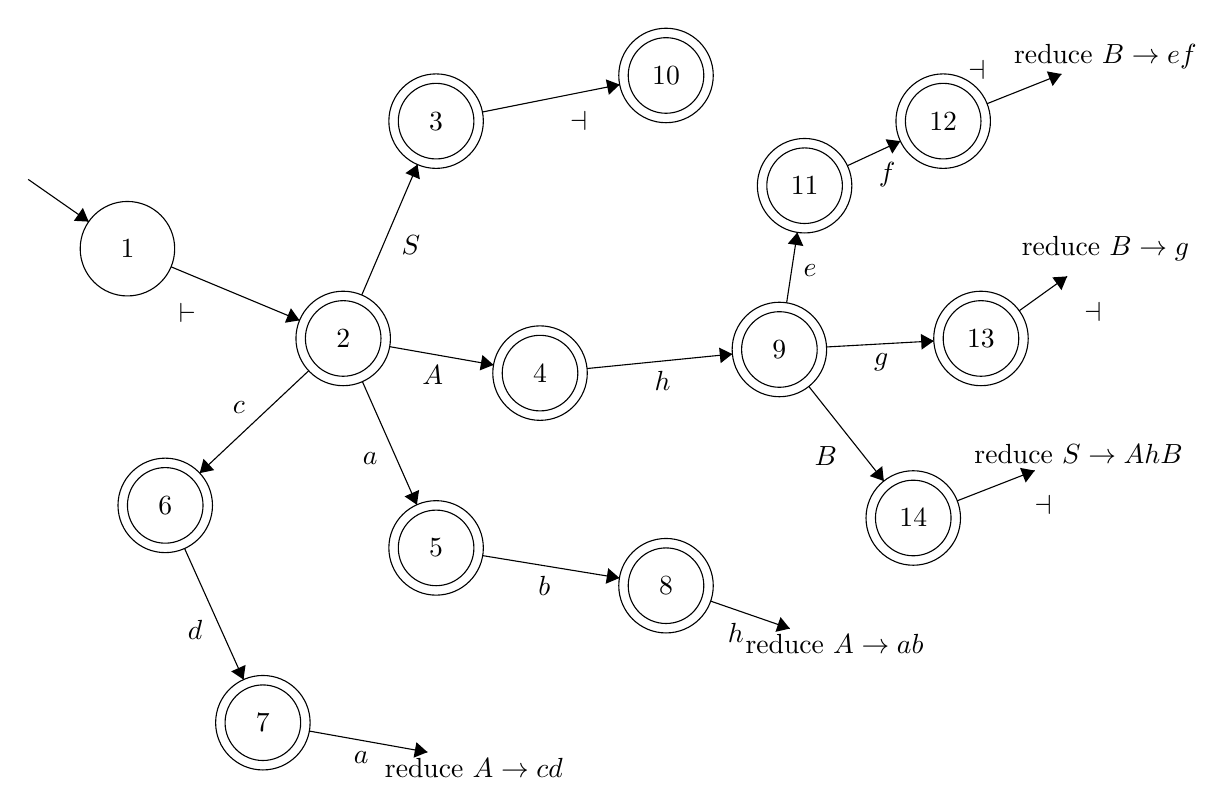
\begin{tikzpicture}[scale=0.2]
						\tikzstyle{every node}+=[inner sep=0pt]
						\draw [black] (10.9,-15.8) circle (3);
						\draw (10.9,-15.8) node {$1$};
						\draw [black] (24.6,-21.5) circle (3);
						\draw (24.6,-21.5) node {$2$};
						\draw [black] (24.6,-21.5) circle (2.4);
						\draw [black] (13.3,-32.1) circle (3);
						\draw (13.3,-32.1) node {$6$};
						\draw [black] (13.3,-32.1) circle (2.4);
						\draw [black] (30.5,-7.7) circle (3);
						\draw (30.5,-7.7) node {$3$};
						\draw [black] (30.5,-7.7) circle (2.4);
						\draw [black] (37.1,-23.7) circle (3);
						\draw (37.1,-23.7) node {$4$};
						\draw [black] (37.1,-23.7) circle (2.4);
						\draw [black] (30.5,-34.8) circle (3);
						\draw (30.5,-34.8) node {$5$};
						\draw [black] (30.5,-34.8) circle (2.4);
						\draw [black] (45.1,-4.8) circle (3);
						\draw (45.1,-4.8) node {$10$};
						\draw [black] (45.1,-4.8) circle (2.4);
						\draw [black] (52.3,-22.2) circle (3);
						\draw (52.3,-22.2) node {$9$};
						\draw [black] (52.3,-22.2) circle (2.4);
						\draw [black] (45.1,-37.2) circle (3);
						\draw (45.1,-37.2) node {$8$};
						\draw [black] (45.1,-37.2) circle (2.4);
						\draw [black] (19.5,-45.9) circle (3);
						\draw (19.5,-45.9) node {$7$};
						\draw [black] (19.5,-45.9) circle (2.4);
						\draw [black] (53.9,-11.8) circle (3);
						\draw (53.9,-11.8) node {$11$};
						\draw [black] (53.9,-11.8) circle (2.4);
						\draw [black] (62.7,-7.7) circle (3);
						\draw (62.7,-7.7) node {$12$};
						\draw [black] (62.7,-7.7) circle (2.4);
						\draw [black] (65.1,-21.5) circle (3);
						\draw (65.1,-21.5) node {$13$};
						\draw [black] (65.1,-21.5) circle (2.4);
						\draw [black] (60.8,-32.9) circle (3);
						\draw (60.8,-32.9) node {$14$};
						\draw [black] (60.8,-32.9) circle (2.4);
						\draw (32.9,-48.8) node {reduce $A \to cd$};
						\draw (55.8,-40.9) node {reduce $A \to ab$};
						\draw (71.3,-28.8) node {reduce $S \to AhB$};
						\draw (73,-15.8) node {reduce $B \to g$};
						\draw (73,-3.6) node {reduce $B \to ef$};
						\draw [black] (4.6,-11.4) -- (8.44,-14.08);
						\fill [black] (8.44,-14.08) -- (8.07,-13.21) -- (7.5,-14.03);
						\draw [black] (13.67,-16.95) -- (21.83,-20.35);
						\fill [black] (21.83,-20.35) -- (21.28,-19.58) -- (20.9,-20.5);
						\draw (14.71,-19.2) node [below] {$\vdash$};
						\draw [black] (22.41,-23.55) -- (15.49,-30.05);
						\fill [black] (15.49,-30.05) -- (16.41,-29.86) -- (15.73,-29.14);
						\draw (17.98,-26.32) node [above] {$c$};
						\draw [black] (14.53,-34.84) -- (18.27,-43.16);
						\fill [black] (18.27,-43.16) -- (18.4,-42.23) -- (17.49,-42.64);
						\draw (15.68,-40) node [left] {$d$};
						\draw [black] (22.45,-46.43) -- (29.95,-47.77);
						\fill [black] (29.95,-47.77) -- (29.25,-47.14) -- (29.07,-48.12);
						\draw (25.74,-47.69) node [below] {$a$};
						\draw [black] (25.82,-24.24) -- (29.28,-32.06);
						\fill [black] (29.28,-32.06) -- (29.42,-31.12) -- (28.5,-31.53);
						\draw (26.82,-29.14) node [left] {$a$};
						\draw [black] (33.46,-35.29) -- (42.14,-36.71);
						\fill [black] (42.14,-36.71) -- (41.43,-36.09) -- (41.27,-37.08);
						\draw (37.37,-36.59) node [below] {$b$};
						\draw [black] (47.94,-38.18) -- (52.96,-39.92);
						\fill [black] (52.96,-39.92) -- (52.37,-39.19) -- (52.05,-40.13);
						\draw (49.54,-39.58) node [below] {$h$};
						\draw [black] (27.55,-22.02) -- (34.15,-23.18);
						\fill [black] (34.15,-23.18) -- (33.44,-22.55) -- (33.27,-23.53);
						\draw (30.28,-23.21) node [below] {$A$};
						\draw [black] (40.09,-23.41) -- (49.31,-22.49);
						\fill [black] (49.31,-22.49) -- (48.47,-22.08) -- (48.57,-23.07);
						\draw (44.88,-23.53) node [below] {$h$};
						\draw [black] (54.17,-24.55) -- (58.93,-30.55);
						\fill [black] (58.93,-30.55) -- (58.83,-29.61) -- (58.04,-30.24);
						\draw (55.99,-28.97) node [left] {$B$};
						\draw [black] (63.59,-31.81) -- (68.51,-29.89);
						\fill [black] (68.51,-29.89) -- (67.58,-29.72) -- (67.94,-30.65);
						\draw (69.04,-31.41) node [below] {$\dashv$};
						\draw [black] (55.3,-22.04) -- (62.1,-21.66);
						\fill [black] (62.1,-21.66) -- (61.28,-21.21) -- (61.33,-22.21);
						\draw (58.76,-22.4) node [below] {$g$};
						\draw [black] (67.53,-19.74) -- (70.57,-17.56);
						\fill [black] (70.57,-17.56) -- (69.63,-17.62) -- (70.21,-18.43);
						\draw (72.2,-19.15) node [below] {$\dashv$};
						\draw [black] (52.76,-19.23) -- (53.44,-14.77);
						\fill [black] (53.44,-14.77) -- (52.83,-15.48) -- (53.82,-15.63);
						\draw (53.8,-17.2) node [right] {$e$};
						\draw [black] (56.62,-10.53) -- (59.98,-8.97);
						\fill [black] (59.98,-8.97) -- (59.04,-8.85) -- (59.47,-9.76);
						\draw (59.14,-10.26) node [below] {$f$};
						\draw [black] (65.49,-6.59) -- (70.21,-4.71);
						\fill [black] (70.21,-4.71) -- (69.28,-4.54) -- (69.65,-5.47);
						\draw (64.84,-5.09) node [above] {$\dashv$};
						\draw [black] (25.78,-18.74) -- (29.32,-10.46);
						\fill [black] (29.32,-10.46) -- (28.55,-11) -- (29.47,-11.39);
						\draw (28.28,-15.55) node [right] {$S$};
						\draw [black] (33.44,-7.12) -- (42.16,-5.38);
						\fill [black] (42.16,-5.38) -- (41.28,-5.05) -- (41.47,-6.03);
						\draw (39.55,-7.03) node [below] {$\dashv$};
						\end{tikzpicture}
						\end{center}

						This DFA recognizes two different things: valid stacks \emph{and} stacks ending in right-hand sides of rules.
				\end{ex}

				Goto[state, symbol] $\to$ state: this is the same DFA transition function from before.
				\\ \\
				Reduce[state, symbol] $\to 2^R$: yields a set of rules to reduce. If |Reduce[s, a]| > 1, then we have a reduce conflict (the oracle can't decide between two rules to reduce) which means this is not an LR(1) grammar. If |Reduce[s, a]| > 0 and Goto[s, a] $\in$ f, then we have a shift/reduce conflict.
				\\ \\
				If you have no conflicts, then you have a deterministic LR(1) parser. With conflicts, you could make a nondeterministic parser which would be inefficient and not LR(1).
				\\ \\
				Here's the pseudocode for an LR(1) parser for input $x$: \\
				\begin{algorithm}[H]
					push $\vdash$\;
					\For{$c$ in $x \dashv$}{
						\While{Reduce[top of state stack, c] = $\set{A \to \alpha}$}{
							pop both stacks $|\alpha|$ times\;
							push Goto[top of state stack, c]\;
						}
						assert Goto[top of state stack, c] $\in$ f; // if not, then $x \not \in L(G)$ \\
					}
					accept if all assertions succeeded\;
				\end{algorithm}

				In an LR(1) parse, if you ever shift $\dashv$, you know for a fact that your parse succeeded.
		\subsection{Building a Parse Tree From a Bottom-Up Parse} \lecture{March 11, 2013}
			A parse tree is a much more general and flexible representation over a rightmost reversed derivation.
			\\ \\
			\underline{Key}: in addition to the (parse) stack, use a parallel tree stack. For every symbol on the stack, we'll have a corresponding parse (sub)tree on the tree stack.

			\begin{ex}
				We have an augmented grammar with this set of rules $R$:
				\begin{align*}
					S' &\to{} \vdash S \dashv \\
					S &\to AhB \\
					A &\to ab \\
					A &\to cd \\
					B &\to ef \\
					B &\to g
				\end{align*}

				If we have input $x = abhg$, the outputted parse tree should be as follows.
				\begin{figure}[H]
					\Tree [.S [.A [.a ] [.b ] ] [.h ] [.B [.g ] ] ]
				\end{figure}

				The parse would be as follows.
				\begin{center}
					\begin{tabular}{|c|c|c|c|c|}
						\hline
						tree stack & parse stack & input read & input not read & action \\ \hline
						$\vdash$ & $\vdash$ & $\epsilon$ & abhg $\dashv$ & initialization \\
						$\vdash$ a & $\vdash$ a & a & bhg $\dashv$ & shift a \\
						$\vdash$ ab & $\vdash$ ab & ab & hg $\dashv$ & shift b \\
						$\vdash$ \Tree [.A [.a ] [.b ] ] & $\vdash$ A & ab & hg $\dashv$ & reduce $A \to ab$ \\
						$\vdash$ \Tree [.A [.a ] [.b ] ] h & $\vdash$ Ah & abh & g $\dashv$ & shift h \\
						$\vdash$ \Tree [.A [.a ] [.b ] ] hg & $\vdash$ Ahg & abhg & $\dashv$ & shift g \\
						$\vdash$ \Tree [.A [.a ] [.b ] ] h \Tree [.B [.g ] ] & $\vdash$ AhB & abhg & $\dashv$ & reduce $B \to g$ \\
						$\vdash$ \Tree [.S [.A [.a ] [.b ] ] [.h ] [.B [.g ] ] ] & $\vdash$ S & abhg & $\dashv$ & reduce $S \to AhB$ \\
						$\vdash$ \Tree [.S [.A [.a ] [.b ] ] [.h ] [.B [.g ] ] ] $\dashv$ & $\vdash$ S $\dashv$ & abhg $\dashv$ & $\epsilon$ & shift $\dashv$ \\ \hline
					\end{tabular}
				\end{center}
			\end{ex}

			To construct the tree stack, you'll likely want to use a linked implementation to make reference to the structures you built up in previous steps.
			\\ \\
			The pseudocode for building a parse tree is as follows. \\ \\
			\begin{algorithm}[H]
				stack = Goto[stack, $\vdash$]\;
				tree\_stack = makeleaf($\vdash$)\;

				\For{every $c$ in $x \dashv$}{
					\While{reduce $A \to \alpha$}{
						// LR(1) reduction: \\
						pop $|\alpha|$ symbols from stack\;
						push Goto[top of stack, c]\;

						// Tree build: \\
						pop $|\alpha|$ subtrees from the tree\_stack\;
						push makenode(root = A, subtrees = nodes that were just popped)\;
					}
					push Goto[top of stack, c]\;
					push makeleaf(c) onto tree\_stack\;
				}
				// Parse tree is now the second element on the tree\_stack. \\
				pop tree\_stack\;
				// Parse tree is now on the top of the tree\_stack.
			\end{algorithm}
			To perform syntax-directed translation, you just need to traverse the parse tree to determine meaning for each subtree.

			\subsubsection{Notes about Assignment 8}
				Questions 1 and 2 are about reversed rightmost derivations, with the questions being similar to ones asked on assignment 7.
				\\ \\
				Question 3 asks you to write a LR(1) parser. You're given a context-free grammar (CFG) and an LR(1) DFA (including Reduce and Goto). If $x \in L(G)$, you'll have to output a derivation for $x$.
				\\ \\
				Question 4 asks you to write a parser for WLPP. The input will be the output from the scanners we used in assignment 6. The output must be a WLPPI file, which is very much like a CFG file \textendash{} it contains a leftmost derivation. You're given the grammar and a DFA, but you're not allowed to read the DFA from a file. You may want to write a program to generate the relevant code for including the DFA in your parser.
				\\ \\
				Note that for question 4, you need to produce a leftmost derivation. However, you would have already built a LR(1) parser for question 3. So, use your parser to build a parse tree and then perform a pre-order traversal to get a leftmost derivation.

			\subsubsection{How to Construct the LR(1) DFA (SLR(1) Method)}
				% Not included on the exam, but for your interest / possible use on assignments.
				There are three basic steps to constructing a LR(1) DFA using the SLR(1) method:
				\begin{enumerate}
					\item Define an NFA that recognizes valid stacks (it implements the shift operation).
					\item Convert the NFA to a DFA with subset construction.
					\item Add extra transition states indicating when to reduce.
				\end{enumerate}

				For each rule in the grammar you're given, you must construct several rules each placing a dot in a unique position on the right-hand side of the rule. These will represent states in the DFA.
				\\ \\
				Here are the states for the augmented grammar presented earlier.
				\begin{align*}
					S' &\to . \vdash S \dashv \\
					S' &\to{} \vdash . S \dashv \\
					S' &\to{} \vdash S . \dashv \\
					S' &\to{} \vdash S \dashv .
					\\ \\
					S &\to .AhB \\
					S &\to A.hB \\
					S &\to Ah.B \\
					S &\to AhB.
					\\ \\
					A &\to .ab \\
					A &\to a.b \\
					A &\to ab.
					\\ \\
					A &\to .cd \\
					A &\to c.d \\
					A &\to cd.
					\\ \\
					B &\to .ef \\
					B &\to e.f \\
					B &\to ef.
					\\ \\
					B &\to .g \\
					B &\to g.
				\end{align*}

				Whenever you have a dot preceding a symbol, you move the dot to the other side of that symbol and make \emph{that} rule a final state.
				\\ \\
				Whenever you have a dot before a nonterminal, you also add an $\epsilon$-transition to rules that have the corresponding nonterminal as their left-hand side.
				\\ \\
				To convert the NFA to a DFA, use subset construction. Since we have $\epsilon$ transitions, you'll also need to take $\epsilon$-closure into account. Once all the states are built up with subset construction, you'll also want transitions to reduction rules for $A$ (for example) on a symbol $h$ (for example) if $h \in \text{follow}(A)$.
				\\ \\
				It \emph{might} be time to perform a reduction when you're on the very right side of the rule. Don't go down a blind alley, though \textendash{} consult your follow function to ensure a reduction is desired.

	\section{The Big Picture: Building a Compiler} \lecture{March 13, 2013}
		At the end of the day, we want to be able to take a WLPP source file, send it into a compiler, and get MIPS assembly object code, which has equivalent meaning. We could then take the produced object code and send it into an assembler to get MIPS binary machine code, if we wanted.
		\\ \\
		The compiler portion consists of a scanner (from A7), which produces some output that will be fed into a parser (from A8), which will produce a WLPPI file. The WLPPI file will be the input for context sensitive analysis (from A9), which will produce a symbol table and a decorated parse tree, both of which will be fed into synthesis (from A10 and A11), where code generation occurs.

		\subsection{Context-Sensitive Analysis}
			Context-sensitive analysis involves all syntax rules that are not conveniently expressed (or are not possible to express) in the scanner and parser. In WLPP, these are rules pertaining to symbols and their types.
			\\ \\
			Symbols have the following rules:
			\begin{itemize}
				\item Every symbol that is used must be declared.
				\item Every symbol that is declared must be declared at most once.
			\end{itemize}

			Types have the following rule:
			\begin{itemize}
				\item Every expression must have a valid type. In WLPP, types are \verb+int+ and \verb+int*+.
			\end{itemize}

			There are many other context-sensitive rules for WLPP \textendash{} refer to the \href{https://www.student.cs.uwaterloo.ca/~cs241/wlpp/WLPP.html}{WLPP specification}.

			\subsubsection{Building a Symbol Table}
				We'll use syntax-directed translation to gather all symbols. During this process, we'll ensure each symbol is declared only once. We'll then create a multiset of symbols.
				\\ \\
				Let's say we have this parse (sub)tree:
				\begin{figure}[H]
					\Tree [.dcl [.type [.INT ] ] [.ID ] ]
				\end{figure}

				Each terminal symbol (ID) will be annotated with its lexeme, such as \verb+fred+. As we come across each symbol, our multiset begins to get constructed: symbols= = $\set{\text{fred}}$.
				\\ \\
				Now, suppose we have the following production rule:
				\begin{align*}
					\text{dcls} \to \text{dcls dcl BECOMES INT SEMI}
				\end{align*}

				This rule would give us the following parse tree:
				\begin{figure}[H]
					\qroofx=2
					\qroofy=2
					\Tree [.dcls [.dcls \qroof{(\{wilma, pebbles\})}. ] [.dcl \qroof{(\{fred\})}. ] [.BECOMES ] [.INT ] [.SEMI ] ]
				\end{figure}

				We recursively determine the symbols for the subtrees, and then decorate the root element with the complete symbol list (the union of the symbol lists of the subtrees). Since this is a multiset, you can check to ensure there were no duplicate declarations. This ensures the second rule for symbols was not violated.
				\\ \\
				Each expression gets a type evaluated for it:
				\begin{align*}
					\underbrace{\underbrace{1}_{\text{type = int}} + \underbrace{2}_{\text{type = int}}}_{\text{type = int}}
				\end{align*}

				This gets slightly more complicated when we don't have constants. For instance:
				\begin{align*}
					\underbrace{1}_{\text{type = int}} + \underbrace{\text{fred}}_{\text{type TBD}}
				\end{align*}

				Note that in this case, we need to check our symbol table for \verb+fred+'s type, to determine if it's \verb+int+ or \verb+int*+. So, the symbol table will need to keep track of each symbol's identifier and type (and value as well).
				\\ \\
				Suppose we have this expression:
				\begin{align*}
					\underbrace{\text{wilma}}_{\text{type TBD}} + \underbrace{\text{fred}}_{\text{type TBD}}
				\end{align*}

				We could construct a table to represent all of the possibilities:
				\begin{center}
					\begin{tabular}{|c|c|c|}
						\hline
						\textbf{wilma} & \textbf{fred} & \textbf{result} \\ \hline
						int & int & int \\
						int & int* & int* \\
						int* & int & int* \\
					int* & int* & error \\ \hline
					\end{tabular}
				\end{center}

				Note that this last entry is an error because adding two pointers together does not make any sense.
				\\ \\
				Let's look at another example. Let's say we have this expression:
				\begin{align*}
					\underbrace{\text{betty}}_{\text{type TBD}} - \underbrace{\text{barney}}_{\text{type TBD}}
				\end{align*}

				Once again, we could construct a table to represent all of the possibilities:
				\begin{center}
					\begin{tabular}{|c|c|c|}
						\hline
						\textbf{betty} & \textbf{barney} & \textbf{result} \\ \hline
						int & int & int \\
						int* & int & int* \\
						int & int* & error \\
						int* & int* & int \\ \hline
					\end{tabular}
				\end{center}

				In this example, the error is caused by the fact that no negative pointers exist. The \verb+int* int*+ case is valid in this example because subtracting one pointer from another results in an integer offset value.
		\subsection{Code Generation} \lecture{March 15, 2013}
			Let's say our compiler is given the following WLPP source code.
			\begin{verbatim}
			int wain(int a, int b) {
			    return 1 + 2;
			}
			\end{verbatim}

			We expect the compiler to output object code. Ideally, we'd get object code like this:
			\begin{verbatim}
			lis $3
			.word 3
			jr $31
			\end{verbatim}

			Throughout the code generation process, we're going to obey our usual MIPS conventions. That is, \$1 and \$2 are input parameter registers, \$3 is the register containing the returned value (or value to return), \$30 is a stack, and \$31 is a return address.
			\\ \\
			Generating the object code described above is quite difficult. Instead, our compilers will likely produce much more verbose (but functionally equivalent) code like this:
			\begin{verbatim}
			lis $4
			.word 4
			lis $3  ;; expr -> term -> factor -> NUM (1) subtree
			.word 1
			sw $3, -4($30)
			sub $30, $30, $4
			lis $5 ;; term -> factor -> NUM (2) subtree
			.word 2
			add $30, $30, $4
			lw $5, -4($30)
			add $3, $5, $3
			jr $31
			\end{verbatim}

			Note that the annotated lines above correspond to the subtrees in this (partial) parse tree:
			\begin{figure}[H]
				\Tree [.expr [.expr [.term [.factor [.{NUM (1)} ] ] ] ] [.+ ] [.term [.factor [.{NUM (2)} ] ] ] ]
			\end{figure}

			\textbf{Conventions used in this object code}:
			\begin{itemize}
				\item \$4 always contains 4.
				\item Every expr, term, and factor puts its \underline{result} into \$3.
				\item The stack is available as usual.
			\end{itemize}

			In reality, we don't care about sub-subtrees. We only really care about this subtree, with the expr and term decorated with the associated code from the sub-subtree which is now hidden:
			\begin{figure}[H]
				\qroofx=5
				\qroofy=5
				\Tree [.expr [.{expr (C1)} \qroof{?}. ] [.+ ] [.{term (C2)} \qroof{?}. ] ] \\
			\end{figure}

			In the above tree, C1 is decorating that instance of expr with:
			\begin{verbatim}
			lis $3
			.word 1
			\end{verbatim}

			Similarly, C2 is decorating that instance of term with:
			\begin{verbatim}
			lis $3
			.word 2
			\end{verbatim}

			The code produced follows this general format:
			\begin{verbatim}
			;; prologue code goes here (set $4, save registers, etc.)
			lis $3
			.word 1
			sw $3, -4($30) ;; save value on stack
			sub $30, $30, $4

			lis $3
			.word 2
			add $30, $30, $4
			lw $5, -4($30)

			add $3, $3, $5
			;; return housekeeping code goes here
			\end{verbatim}

			We'll define the \& symbol to mean concatenation, in this case.
			\\ \\
			Code ($\text{expr}_0 \to \text{expr}_1 + \text{term})$ =
			\begin{verbatim}
			code(expr_1) &
			"sw $3, -4($30)
			sub $30, $30, $4" & ;; push $3
			code(term) &
			"add $30, $30, $4
			lw $5, -4($30)" &   ;; pop $3
			"add $3, $5, $3"    ;; code(+)
			\end{verbatim}

			Similarly, Code($\text{procedure} \to \ldots$) =
			\begin{verbatim}
			"lis $4
			.word 4" & ;; prologue
			code(dcl_1) &
			code(dcl_2) &
			code(dcls) &
			code(statements) &
			code(expr) &
			"jr $31" ;; epilogue
			\end{verbatim}

			An alternate way of generating Code($\text{expr} \to \text{expr} + \text{term}$) =
			\begin{verbatim}
			code(term) &
			"sw $3, -4($30)
			sub $30, $30, $4" &
			code(expr) &
			"add $30, $30, $4 ;; pop stack
			lw $5, -4($30)
			add $3, $3, $5"   ;; perform addition
			\end{verbatim}

			Let's examine the following WLPP code:
			\begin{verbatim}
			int wain(int a, int b) {
			    return a + b;
			}
			\end{verbatim}

			Let's look at more conventions, specifically how to represent parameters. For now (and we'll change this later when we represent variables), \$1 is the first parameter and \$2 is the second parameter. We're going to need to expand our symbol table to include how each symbol is represented:

			\begin{center}
				\begin{tabular}{|c|c|c|}
					\hline
					Symbol & Type & Representation \\ \hline
					a & int & \$1 \\
					b & int & \$2 \\ \hline
				\end{tabular}
			\end{center}

			Now, we can look at Code($\text{factor} \to \text{ID}$) =
			\begin{verbatim}
			"add $3, $0, " & representation(lexeme(ID)) ;; lookup in symbol table
			\end{verbatim}

			For example, for variable a, Code(a) = \verb+add $3, $0, $1+, and for variable b, Code(b) = \verb+add $3, $0, $2+.
			\\ \\
			This assumes our variables are stored in registers. This is only the case for now, and only for \verb+wain+'s parameters. Later, once we start storing all variables on the stack, we'll need to perform a \verb+lw+ to fetch the data from the stack, placing the result in \$3.
			\\ \\
			So, the object code equivalent to the WLPP program above is:
			\begin{verbatim}
			lis $4
			.word 4
			add $3, $0, $1
			sw $3, -4($30)
			sub $30, $30, $4
			add $3, $0, $2
			add $30, $30, $4
			lw $5, -4($30)
			add $3, $5, $3
			jr $31
			\end{verbatim}

			\textbf{Code Generation Conventions So Far}: \lecture{March 18, 2013}
			\begin{itemize}
				\item \$1 \textendash{} first parameter (to be changed).
				\item \$2 \textendash{} second parameter (to be changed).
				\item \$3 \textendash{} result from every code fragment.
				\item \$4 \textendash{} contains 4 (for use when we're constantly pushing/popping the stack).
				\item \$30 \textendash{} stack. Use as necessary, but reset \$30 after every code fragment.
				\item \$31 \textendash{} return address. Do not clobber.
				\item Every result is an int (to be changed since int* is also a type in WLPP).
			\end{itemize}

			The three conventions that I said we'll change were simplifying assumptions we made earlier. We're going to change those assumptions a bit now.

			\subsubsection{Variables}
				Variables have declarations and uses, which need to be handled in different ways.
				\\ \\
				Take this code, for instance:
				\begin{verbatim}
				int fred = 17;
				int* barney = NULL;
				\end{verbatim}

				The decorated parse tree for the first line in the code snippet above is:
				\begin{figure}[H]
					\Tree [.dcls [.dcls ] [.{dcl (fred : int)} [.{type (int)} [.INT ] ] [.{ID (fred)} ] ] [.BECOMES ] [.{NUM (17)} ] [.SEMI ] ]
				\end{figure}

				We will have constructed our symbol table to be:
				\begin{center}
					\begin{tabular}{|c|c|}
						\hline
						\textbf{Symbol} & \textbf{Type} \\ \hline
						fred & int \\
						barney & int* \\ \hline
					\end{tabular}
				\end{center}

				First, we perform the context-sensitive analysis. This ensures that (int, 17) and (int*, barney) are valid pairings.
				\\ \\
				Next, we need to pick a representation for the variables. Note that we can't use registers only because there are a finite number of them. Instead, we should use RAM. We could use both, but we won't because it's simpler to keep all of our variables in one place.
				\\ \\
				There are two choices for selecting locations in RAM to store variables:
				\begin{itemize}
					\item Declare a garbage \verb+.word+. However, these variables will act as static variables, which is not always desired (especially when handling recursive programs).
					\item Use the stack. We're going to use the \textbf{stack frame storage allocation} algorithm.
				\end{itemize}

				At entry to the prologue of our code, we have a stack pointer, \$30. We'll reserve a large block of storage \textendash{} enough for every variable \textendash{} on the stack, called a stack frame.
				\\ \\
				To do this, we decrement the stack pointer (\$30) to below the stack frame and we store a \textbf{frame pointer} in a different register (say, \$29).
				\\ \\
				Suppose there are $n$ declared variables in our program. We must arbitrarily assign each variable a distinct number $0 \le i < n$. The address in RAM of variable $i$ is $4i + \$29$. Let's say our symbol table now contains:
				\begin{center}
					\begin{tabular}{|c|c|c|}
						\hline
						\textbf{Symbol} & \textbf{Type} & $\boldsymbol{i}$ \\ \hline
						fred & int & 0 \\
						barney & int* & 1 \\ \hline
					\end{tabular}
				\end{center}

				The address of fred in RAM would be $4(0) + \$29 = \$29$. The address for barney would be $4(1) + \$29 = 4 + \$29$.
				\\ \\
				The MIPS assembly code to get the value of a variable would be \verb+lw $3, 4i($29)+. Similarly, the assembly code to place a variable into RAM would be \verb+sw $5, 4i($29)+, where \$5 is a register holding the value of the variable presently.
				\\ \\
				There is a gotcha with this approach, however. The value of 4i in the \verb+lw+ instruction must be a 16-bit number, which means we can only create $\approx 8,000$ variables using this method. Just between you, me, and Marmoset, there will not be more than 8,000 variables on this assignment, so this approach is okay for our use.
				\\ \\
				What kind of code do we need for all of this? If we have the line \verb+int fred = 17;+, we will construct a symbol table containing just ``fred'' (int) = 0. Once the context-sensitive analysis determines that int and 17 are a valid type match, we can generate the code which will be similar to this:
				\begin{verbatim}
				lis $3
				.word 17
				sw $3, 0($29)
				\end{verbatim}

				Now, suppose instead we have \verb+int* barney = NULL;+. After context-sensitive analysis, we could generate code like this:
				\begin{verbatim}
				add $3, $0, $0 ;; 0 represents NULL in this case
				sw $3, 4($29)
				\end{verbatim}

				Note that the representation for NULL is conventionally zero. This is \emph{okay}, but ideally we'd choose a NULL representation that is not a power of four, so as not to confuse it with an actual memory address.
				\\ \\
				When representing variables of type int*, there are a few possibilities. You could store a word number, or an offset in an array, but it's highly recommended that you store the RAM address itself.
				\\ \\
				What about \verb+wain+'s parameters? We have the following WLPP code:
				\begin{verbatim}
				int wain(dcl, dcl) {
				    // ...
				}
				\end{verbatim}

				Each \verb+dcl+ expands into a parse subtree like these:
				\begin{figure}[H]
					\Tree [.dcl [.type [.INT ] [.$\star$ ] ] [.{ID (homer)} ] ]
					\Tree [.dcl [.type [.INT ] ] [.{ID (marge)} ] ]
				\end{figure}

				Earlier, we represented \verb+homer+ as \$1 and \verb+marge+ as \$2. However, we want to treat these just like the other variables, by storing them in RAM. Just like normal variable declarations, they are assigned $i$ values and are placed in RAM accordingly. For example, if the $i$ values were 2 and 3 for \verb+homer+ and \verb+marge+, respectively, then the following MIPS code would place them in RAM.
				\begin{verbatim}
				sw $1, 8($29)  ;; homer
				sw $2, 12($29) ;; marge
				\end{verbatim}

				Now, let's look at another simplification we made earlier: the plus operation. Suppose we had the code \verb|homer + marge|. The MIPS assembly code that could be produced is Code(homer + marge) =
				\begin{verbatim}
				lw $3, 8($29)  ;; homer
				sw $3, -4($30) ;; push $3 onto stack
				sub $30, $30, $4
				lw $3, 12($29)
				add $30, $30, $4
				lw $5, -4($30) ;; pop into $5
				add $3, $3, $3 ;; multiply
				add $3, $3, $3 ;; by 4
				add $3, $5, $3
				\end{verbatim}

				When generating MIPS assembly code for \verb|expr + term|, you must perform many comparisons to determine how to handle various types. The algorithm for this would be something like this: \\
				\begin{algorithm}[H]
					\uIf{type(expr) == int*}{
						\If{type(term) == int}{
							// ...
						}
					}
					\uElseIf{type(expr) == int and type(term) == int}{
						// ...
					}
					\uElseIf{...various other cases...}{
						// ...
					}
					\Else{ERROR}
				\end{algorithm}

				This is an important step because the code you generate will actually differ depending on the combination of types.
				\\ \\
				When performing context-sensitive analysis, don't recompute the type all over the place (such as in recursive calls). Decorate your parse tree instead. Also, make sure you're passing around reference parameters whenever possible. Otherwise, you'll end up with a program with worse complexity. \lecture{March 20, 2013}
				\\ \\
				We have (at least) two choices when generating Code(expr + term). The first approach evaluates expr first:
				\begin{verbatim}
				code(expr)
				push $3
				code(term)
				pop $5
				add $3, $5, $3
				\end{verbatim}

				Or, we could evaluate the second operand (term) first:
				\begin{verbatim}
				code(term)
				push $3
				code(expr)
				pop $5
				add $3, $3, $5
				\end{verbatim}

				This applies similarly for subtraction and multiplication. You shouldn't assume commutability for the \verb+add+ instruction \textendash{} pass the operands in their correct order, even if it does not matter in some cases. In general, for Code(foo OP bar), we have the choice between:
				\begin{verbatim}
				code(foo)
				push
				code(bar)
				pop
				operations for OP
				\end{verbatim}

				And:
				\begin{verbatim}
				code(bar)
				push
				code(foo)
				pop
				operations for OP
				\end{verbatim}

				Moving along, we also can trivially determine these code fragments:
				\begin{itemize}
					\item Code(expr $\to$ term) = Code(term)
					\item Code(term $\to$ factor) = Code(factor)
					\item Code(factor $\to$ LPAREN expr RPAREN) = Code(expr)
				\end{itemize}

				You might be able to be clever and make your compiler look ahead and realize that Code(bar) doesn't use \$6 (for instance), so Code(foo) could put its result in \$6 directly in order to skip the stack steps. This might be something to try for the bonus, but otherwise, use the \$3 stack-based approach for simplicity to get things working.

			\subsubsection{Statements}
				Let's look at printing next. We don't want to reproduce all the print code every time we want to print something. Instead, we'll use a procedure. Recall the WLPP grammar rule for printing:
				\begin{align*}
					\text{statement} &\to \text{PRINTLN LPAREN expr RPAREN SEMI} \\
				\end{align*}

				Also, recall the generalized code for an arbitrary procedure:
				\begin{verbatim}
				;; prologue
				push $31
				  .
				  .
				  .
				;; epilogue
				pop $31
				jr $31
				print: ...
				\end{verbatim}

				So, Code(statement $\to$ PRINTLN LPAREN expr RPAREN SEMI) =
				\begin{verbatim}
				code(expr)
				add $1, $3, $0 ;; set up the parameter for the print procedure
				lis $5
				.word print
				jalr $5        ;; clobbers $31
				\end{verbatim}

				Note that we changed \$1! That was the parameter for wain. However, remember we earlier placed \$1's value into a variable on the stack, so everything's okay.
				\\ \\
				\verb+jalr $5+ clobbers \$31. This isn't a huge problem, all we have to do is push \$31 onto our stack in the prologue and pop it just prior to the \verb+jr $31+ call in our prologue.
				\\ \\
				Let's generate the code for the rule: statements $\to$ statements statement. The safest choice for this would be to generate:
				\begin{verbatim}
				code(statements)
				code(statement)
				\end{verbatim}

				What if we wanted to generate the code differently such that the statement's code was placed prior to the rest of the statements? That is, what if we wanted to generate code like this:
				\begin{verbatim}
				code(statement)
				code(statements)
				\end{verbatim}

				Is that correct? It might be. We have no way of guaranteeing it in every case. The order of some object code matters, sometimes. It's generally unsafe to do this.
				\\ \\
				Let's look at this rule: statement $\to$ lvalue BECOMES expr SEMI. We first need to decide on a representation for an lvalue. Here are all the rules for what an lvalue can be:
				\begin{align*}
					\text{lvalue} &\to \text{ID} \\
					\text{lvalue} &\to \text{STAR factor} \\
					\text{lvalue} &\to \text{LPAREN lvalue RPAREN}
				\end{align*}

				How should we represent an lvalue? Well, we can't just place them in registers, for a couple of reasons. First, there is the limitation on the number of registers we have available for our use. More importantly, however, is the fact that when we change the value (since an lvalue by definition is going to be changed), we want it to be updated in its permanent location in RAM.
				\\ \\
				We'll take the stupidly simple approach of making each lvalue an address in RAM.
				\\ \\
				Let's determine Code(statement $\to$ lvalue BECOMES expr SEMI):
				\begin{verbatim}
				code(expr)
				push $3
				code(lvalue) ;; places address of lvalue into $3
				pop $5
				sw $5, 0($3)
				\end{verbatim}

				Alternatively, we can switch up the order of evaluation:
				\begin{verbatim}
				code(lvalue)
				push $3
				code(expr)
				pop $5
				sw $3, 0($5)
				\end{verbatim}

				In this case, it doesn't matter whether we evaluate (or generate code) for the lvalue or the expr first, so both of these approaches are equally acceptable.
				\\ \\
				Let's look at Code(lvalue $\to$ ID). We know that variables are just offsets in the stack frame. We can get the offset of the ID from the symbol table. We need the \emph{address} of that location, though. So, we get Code(lvalue $\to$ ID) =
				\begin{verbatim}
				lis $3
				.word offset(ID)
				add $3, $3, $29
				\end{verbatim}

				You may think it'd be easier to just return the offset, rather than a memory address. That isn't easier, however, because we still have the following rules to deal with:
				\begin{itemize}
					\item Code(lvalue $\to$ STAR factor) = Code(factor), with the assertion that type(factor) = int $\star$.
					\item Code(lvalue $\to$ LPAREN lvalue RPAREN) = Code(lvalue).
					\item Code(factor $\to$ AMP lvalue) = Code(lvalue). Note that factor must be of type int $\star$, lvalue must be of type int, and the Code(lvalue) will always contain an address, as needed for these types.
				\end{itemize}

			\subsubsection{Control Structures \& Tests} \lecture{March 22, 2013}
				We want to be able to generate code for rules like this:
				\begin{align*}
					\text{statement} &\to \text{WHILE LPAREN test RPAREN LBRACE statements RBRACE}
				\end{align*}

				We first need to be able to generate code for a test. Let's look at this rule: test $\to \text{expr}_1$ LT $\text{expr}_2$. This allows us to write WLPP code like:
				\begin{verbatim}
				while(a < b) {
				    a = a + 1;
				}
				\end{verbatim}

				A \textbf{test} is essentially a boolean value. We'll follow the convention that a boolean value is represented as 0 = false, 1 = true. Note that this is not exactly how booleans are represented in languages like C++ (where instead, any non-zero value is true).
				\\ \\
				Code(test $\to \text{expr}_1$ LT $\text{expr}_2$):
				\begin{verbatim}
				code(expr_1)
				push $3
				code(expr_2)
				pop $5
				slt $3, $5, $3
				\end{verbatim}

				Now that we've generated the code for a test, we can proceed to generate code different control structures like loops and branching.
				\\ \\
				Code(statement $\to$ WHILE LPAREN test RPAREN LBRACE statements RBRACE):
				\begin{verbatim}
				loop:
				    code(test)
				    beq $3, $0, quit
				    code(statements)
				    beq $0, $0, loop

				quit:
				\end{verbatim}

				There are a couple of problems with the code we generated. If we have multiple loops in our program, we'll have multiple loop and quit labels. To solve this, you should affix a unique identifier to the labels, and for readability, you may want to use the same identifier for the loop/quit labels that correspond with each other.
				\\ \\
				The other problem is if our loop is over $\approx$ 32,000 instructions long, since the $i$ value that \verb+beq+ accepts as its third operand must be a 16-bit integer. Here's one way we could solve this:
				\begin{verbatim}
				loop123:
				    code(test)
				    bne $3, $0, cont123
				    lis $5
				    .word quit123
				    jr $5

				cont123:
				    code(statements)
				    lis $5
				    .word loop123
				    jr $5

				quit123:
				\end{verbatim}

				You could make your code dynamically choose between these two methods, depending of the length of code(statements). All control structures are subject to this caveat.
				\\ \\
				Let's now look at Code(statement $\to$ IF LPAREN test RPAREN LBRACE $\text{statements}_1$ RBRACE ELSE LBRACE $\text{statements}_2$ RBRACE):
				\begin{verbatim}
				    code(test)
				    beq $3, $0, else123
				    code(statements_1) ;; true part
				    beq $0, $0, done123

				else123:
				    code(statements_2) ;; false part

				done123:
				\end{verbatim}

				Alternatively, we could've generated this code:
				\begin{verbatim}
				    code(test)
				    bne $3, $0, true123

				    code(statements_2)
				    beq $0, $0, done123

				true123:
				    code(statements_1)

				done123:
				\end{verbatim}

				The choice between these two is somewhat arbitrary.
				\\ \\
				One other approach to this is to take advantage of places in your code that can contain code that will never be executed (such as after \verb+jr $31+). You could have:
				\begin{verbatim}
				    code(test)
				    bne $3, $0, true123
				                                                true123: ;; out of line, somewhere
				                                                    statements_1
				    statements_2                                    beq $0, $0, done123

				done123:
				\end{verbatim}

				If the true part very rarely occurs, you take zero branches on the else case, which is nice. This would save some execution time.
				\\ \\
				Let's take a look at more test rules.
				\begin{itemize}
					\item Code(test $\to \text{expr}_1$ GT $\text{expr}_2$) $\equiv$ Code(test $\to \text{expr}_2$ LT $\text{expr}_1$).
					\item Code(test $\to \text{expr}_1$ GE $\text{expr}_2$) $\equiv$ not(Code(test $\to \text{expr}_1$ LT $\text{expr}_2$)). According to our convention, 0 = false and 1 = true, so not($x$) = $1 - x$. So, we get:
						\\ \\
						Code(test $\to \text{expr}_1$ GE $\text{expr}_2$):
						\begin{verbatim}
						code(expr_1 LT expr_2)
						lis $11 ;; not $3
						.word 1
						sub $3, $11, $3
						\end{verbatim}

						We should move the populating of \$11 into our prologue, and add \$11 = 1 to our list of conventions.

					\item Code(test $\to \text{expr}_1$ LE $\text{expr}_2$) $\equiv$ Code(test $\to \text{expr}_2$ GE $\text{expr}_1$).
					\item Code(test $\to \text{expr}_1$ NE $\text{expr}_2$) $\equiv$ Code(test $\to \text{expr}_1$ LT $\text{expr}_2$) OR Code(test $\to \text{expr}_2$ LT $\text{expr}_1$). We can generate this code like so:
						\begin{verbatim}
						code(expr_1)
						push $3
						code(expr_2)
						pop $5
						slt $6, $5, $3
						slt $7, $3, $5
						add $3, $6, $7
						\end{verbatim}

						Note that the final line is an OR, except this implementation of OR does not work in general. It only works here because we know both conditions won't be true simultaneously. In other cases, we would need to handle the case where both conditions are true, and then our possible truth values would be 1 and 2.
					\item Code(test $\to \text{expr}$ EQ $\text{expr}_2)$ $\equiv$ not(Code(test $\to \text{expr}_1$ NE $\text{expr}_2$)). The code for this is:
						\begin{verbatim}
						code(expr_1 NE expr_2)
						sub $3, $11, $3
						\end{verbatim}
				\end{itemize}

			\subsubsection{Dynamic Memory Allocation} \lecture{March 25, 2013}
				We only have two WLPP grammar rules left to discuss:
				\begin{align*}
					\text{factor} &\to \text{NEW INT LBRACK expr RBRACK} \\
					\text{statement} &\to \text{DELETE LBRACK RBRACK expr}
				\end{align*}

				You can download \verb+alloc.asm+ for use on the assignments. It contains procedures for \verb+new+ and \verb+delete+. You may want to optimize (rewrite) them for the bonus question.
				\\ \\
				\verb+alloc.asm+ implements three procedures:
				\begin{itemize}
					\item \verb+init+ initializes the allocation code. This must be called prior to any allocations or deletions.
					\item \verb+new+ attempts to allocate $n$ words of storage, where $n = \$1$. It returns a pointer in \$3 if memory was allocated, or NULL otherwise.
					\item \verb+delete+ marks the memory at the address given in \$1 as not needed. The procedure already knows how large the block of memory is. This essentially deletes a pointer that you had allocated earlier in your program.
				\end{itemize}

				``This is the Walmart approach to storage. You want to use it for awhile, so you go, you buy it. Then when you're tired of it, you tape it up again and take it back, and they put it back on the shelf for another customer.'' \verb+new+ and \verb+delete+ do the same thing as Walmart.
				\\ \\
				You'll have to remove the \verb+.import+ and \verb+.export+ statements from \verb+alloc.asm+ prior to including it in your outputted code. Those pseudo-instructions are meant to be used by a linker, but we are not running a linker on our code. Additionally, \verb+alloc.asm+ \emph{must} be physically last in your outputted code.
				\\ \\
				The code for each of the rules above is simply \verb+code(expr)+, followed by a call to \verb+new+ or \verb+delete+ with $n$ or $p$ in \$1, respectively.
	\section{Dynamic Memory Allocation: Implementing Heaps}
		\verb+alloc.asm+ implements a \textbf{heap}, which is an abstract data type (ADT) (not to be confused with the priority queue implementation), which supports the following operations:
		\begin{itemize}
			\item \verb+initialize+.
			\item \verb+finalize+.
			\item \verb+allocate(n)+: finds $n$ available units of RAM, or fails.
			\item \verb+free(p)+: frees the previously allocated RAM that is referred to by $p$.
		\end{itemize}

		The first step to implementing a heap is to identify some available RAM. This RAM is typically in one continuous block, which we will call the \textbf{arena}.
		\\ \\
		Where do we put the arena? It'll have to use some space normally available for the stack. We could create a fixed size arena by dedicating a certain number of words directly above your program's code, and leave the rest of the space for the stack.
		\\ \\
		The given \verb+alloc.asm+ file implements a fixed-size arena. That's why it must be at the very end of our program. It has a label \verb+end:+ at the very bottom of it that indicates where your program ends, which is also where the arena begins.
		\\ \\
		\underline{Aside}: up until this point, we've made the na\"ive assumption that the stack is not bounded. In reality, of course the stack is bounded, but we're not sure how large the stack needs to be, so we've been treating it as unbounded. Also, you should really check for possible stack overflows, otherwise your program could get overwritten by a user and arbitrary code could be executed.
		\\ \\
		You could dedicate half of your stack space (conventionally denoted as the memory below the address stored in \$30) to the arena. The other half will be used for the stack. We will call this the \textbf{split the baby approach}.
		\\ \\
		Alternatively, you could start the arena right after your program and start the stack at \$30, and use the first-come, first-serve approach.

		\subsection{The Loaf of Bread Algorithm}
			The simplest algorithm for \verb+allocate(n)+ is what we will call the \textbf{loaf of bread algorithm}. It's simple: you just give out the memory in order. The chunks of memory you're allocating could potentially be chunks of different sizes.
			\\ \\
			With the loaf of bread algorithm, we can't implement \verb+free(p)+. All sales are final, so to speak.
			\\ \\
			If instead we wanted to implement the Walmart algorithm, we would need to find the most appropriate hole when we want to allocate some memory. What if there are many small holes but we need a large one? That is, the total amount of unused storage in your arena is large enough, but there's no continuous block of RAM available. This is known as \textbf{fragmentation}. \lecture{March 27, 2013}
			\\ \\
			In the simple case, \verb+alloc()+ will allocate $k$ words, where typically $k = 2$. In Lisp or Scheme, \verb+alloc()+ is written as \verb+(cons a b)+. A \verb+cons+ statement allocates two spaces in memory (\verb+first+ \& \verb+rest+, also known as \verb+car+ \& \verb+cdr+).
			\\ \\
			We could create an arena where we have two pointers: a \verb+bread+ pointer (the next slice of bread comes from where the \verb+bread+ pointer is pointing to), and an \verb+end+ pointer. The slice of bread algorithm for \verb+alloc()+ is as follows.

			\begin{algorithm}[H]
				\uIf{bread < end}{
					tmp = bread\;
					bread++\;
					\Return{tmp}
				}
				\Else{fail}
			\end{algorithm}

			The loaf of bread \verb+alloc()+ algorithm runs in O(1) time, as does its \verb+init()+ algorithm (which just populates the \verb+bread+ and \verb+end+ pointers).
			\\ \\
			This algorithm is a bit hostile because it completely ignores \verb+free+s. Storage is never reclaimed.

		\subsection{Available Space List}
			The available space list technique involves building up an array of elements that represent available blocks of memory, split into fixed-size pieces. Each block points to the next one, and we also have three pointers. The \verb+avail+ pointer points to the next available piece of memory. We also have \verb+tmp+ and \verb+i+ pointers, pointing to the end of our list.
			\\ \\
			\verb+init()+ runs in $O(N)$ time, where $N$ is the size of the arena (which is quite slow). It follows this algorithm:

			\begin{algorithm}[H]
				next(1st area) = NULL\;
				\For{i = arena; i < end; i++}{
					next(i-th area) = avail\;
					avail = i-th area\;
				}
			\end{algorithm}

			\verb+alloc()+ runs in constant $O(1)$ time by following this algorithm:

			\begin{algorithm}[H]
				\uIf{avail $\ne$ NULL}{
					tmp = avail\;
					avail = next(avail)\;
					\Return{tmp}
				}
				\Else{fail}
			\end{algorithm}

			\verb+free(p)+ trivially runs in constant $O(1)$ time by following this algorithm:

			\begin{algorithm}[H]
				next(p) = avail\;
				avail = p\;
			\end{algorithm}

			This is all pretty nice, except for \verb+init+. We could take a hybrid approach to make \verb+init+ faster while maintaining the runtimes of the other operations.

		\subsection{Hybrid Loaf of Bread and Available Space List}
			We introduce a \verb+bread+ pointer into our available space list, with it initially being set to the beginning of the arena (the first element).
			\\ \\
			\verb+init()+ now follows this algorithm, which runs in constant $O(1)$ time:

			\begin{algorithm}[H]
				bread = arena\;
				avail = NULL\;
			\end{algorithm}

			\verb+alloc()+ now follows this algorithm, which also runs in constant $O(1)$ time (as before):

			\begin{algorithm}[H]
				\uIf{avail $\ne$ NULL}{
					tmp = avail\;
					avail = next(avail)\;
					\Return{tmp}
				}
				\uElseIf{bread < end}{
					tmp = bread\;
					bread++\;
					\Return{tmp}
				}
				\Else{fail}
			\end{algorithm}

			\verb+free(p)+ operates identically to before, in constant $O(1)$ time:

			\begin{algorithm}[H]
				next(p) = avail\;
				avail = p\;
			\end{algorithm}

			This entire algorithm runs in constant time! However, it's important to remember that this algorithm only works for allocations of fixed size.

		\subsection{Implicit Freedom}
			Modern languages that aren't archaic all have implicit \verb+free+. How does that work?
			\\ \\
			\underline{Key}: find unreferenced storage units (areas that are not pointed to by anyone). We could instead find all of the referenced units, which might be easier.
			\\ \\
			We can use the stack frame (known variables) as \textbf{root pointers}. We can then find all \emph{reachable} units in the arena, and mark them.
			\\ \\
			How do we mark them, exactly? Observe that the last two bits in a pointer must be zero, because every pointer is a multiple of four. We can use these two bits for a sticky note (a ``taken?'' sticky note).
			\\ \\
			This is known as the \textbf{mark and sweep algorithm}.
			\\ \\
			Mark($n$) takes $O(n)$ time, where $n$ is the number of reachable units. Sweep($N$) takes $O(N)$ time, where $N$ is the size of the arena.
			\\ \\
			It would be nice if the runtime of this algorithm was proportional only to the memory we're \emph{actually} using, and not the entire arena.
			\\ \\
			The \emph{average} runtime of this is still $O(1)$, however. This is because we have a lot of really quick operations followed by one occasional \emph{huge} operation.
			\\ \\
			The mark and sweep algorithm is akin to the procrastination algorithm of letting dirty dishes pile up until there are no clean ones left. Better algorithms, such as those used in incremental garbage collectors, do one piece of the garbage collection (marking or sweeping) in each \verb+alloc()+, to distribute the longer time into all of the smaller $O(1)$ \verb+alloc()+ calls.
			\\ \\
			Garbage collection could also be concurrent. ``It's hard to buy a computer that doesn't have 16 cores these days. Let one of your cores be a garbage collector and clean up after you, like a maid or a mother.''

		\subsection{Use Counts}
			Another approach to garbage collection is \textbf{use counts}. We'll start by appending a use count to each piece of allocated storage.
			\\ \\
			In \verb+alloc()+, we set this use count to 1. When we assign a variable away from a piece of memory, we decrement the use count. When we assign a variable to a piece of memory, we increment its use count. Calls to \verb+delete+ will decrement this count.
			\\ \\
			There are two gotchas with this approach:
			\begin{itemize}
				\item We have to store use counts.
				\item It doesn't work for cyclic structures. If we have a data structure that points to another data structure that points back to the first one, the use counts are both at 2, and then when we call \verb+delete+ their use counts both become 1 ($\ne 0$), so they are not freed.
			\end{itemize}

			Use counts are still a perfectly valid idea in cases where we know we won't have cyclic data structures.

		\subsection{Copying Collector}
			As you're using a piece of memory, you copy all of it to a space dedicated for memory that's currently in use. Note that this has the consequence of only letting you effectively use half of the RAM available, maximum.
			\\ \\
			This copying has the effect of relocating code, since code is stored in memory. That might be tough in languages like C++ where memory addresses are part of the language. You could always convert pointers to integers, strings, or do other crazy things (like reverse the bits in a pointer), and the compiler will not be aware of that use.
			\\ \\
			Andrew Appel argued that instead of using the stack (which would involve a push and pop), just use \verb+alloc()+ instead. It's equivalent to just pushing onto the stack, and removes the need for the popping code.

		\subsection{Holes} \lecture{April 3, 2013}
			We will refer to unallocated areas of memory as \textbf{holes}. That is, holes are areas of memory that are available to fill with some new data. In fixed-size memory allocation, all holes have the same size as each other.

		\subsection{Variable-Sized Dynamic Memory Allocation}
			When we start to discuss variable-sized dynamic memory allocation, all of the properties we discussed for fixed-size allocation go out the window. But what would happen if we \emph{tried} to apply the same concepts to variable-sized allocation?
			\\ \\
			The approach of maintaining an available space list is not sufficient anymore. \verb+alloc(n)+ now takes a parameter, $n$, which represents the size of the chunk of memory we want to allocate. The available space list is a linked list connected in the order of deletions, but we don't know how big each hole in that list actually is.
			\\ \\
			We somehow need to find a hole that is at least $n$ bytes large, in order to satisfy the \verb+alloc(n)+ request. In order to do this, we'll have to store the size of each hole.
			\\ \\
			In order to find an appropriate hole, we'll have to search through the available space list (the list of holes). There are a few approaches to this search:
			\begin{itemize}
				\item \textbf{First fit}: choosing the first hole that is big enough. You don't need to pick sides. This approach is easy to implement. This approach also leaves a variety of hole sizes available for future use, which is good.
				\item \textbf{Worst fit}: choosing the biggest hole we can find. This experiences \textbf{hole erosion} \textendash{} that is, all holes will tend to become very similar sizes over time.
				\item \textbf{Best fit}: choosing the smallest hole that's big enough. Most of the time, you'll be able to use most of the hole you selected, but that'll leave a sliver of storage remaining. That sliver will be hard to fill later on. You waste less space now, but more space later (as the slivers accumulate in different areas of your arena).
			\end{itemize}

			The choice between these three approaches is not clear cut because there is no analytical way to compare these.
			\\ \\
			With fixed-size allocation, you'll fail only if all memory is full, since all holes are the same size. With variable-size allocation, you'll fail if there is no hole that is big enough.
			\\ \\
			In archaic languages like C and C++ (that don't have implicit \verb+free+s), \verb+free(p)+ frees the storage area that pointer $p$ points to. How do we know how big that area is, though? We'll need to keep track of the length of those areas as well.
			\\ \\
			So, we'll need to keep track of the length of holes, and the length of allocated areas. We might as well standardize on a way to store these lengths. When you allocate $n$ bytes of storage, you'll actually allocate a few extra bytes that you won't expose to the user. These bytes will act as a header that can contain the length of the block as well as a pointer to the next block in the available space list (and a footer, which will be discussed later).
			\\ \\
			\textbf{Fragmentation} occurs when small holes collectively have enough space to satisfy an \verb+alloc(n)+ request, but no single hole is big enough to satisfy that request. This occurs with the best fit approach because the holes that turn into sliver-holes become smaller and smaller over time.

			\subsubsection{Coalescing Adjacent Holes}
				When you \verb+free+ an area, combine it with adjacent hole(s) if there are any. This has the consequence of no two holes ever being beside each other anymore.
				\\ \\
				The process of coalescing adjacent holes does not guarantee that you'll solve the problem of fragmentation, it only guarantees that you aren't destined to fail.
				\\ \\
				There are a few cases to consider when you're trying to \verb+free+ an area pointed to by $p$:
				\begin{itemize}
					\item $p$ is surrounded by two holes. This results in one single hole as $p$ is freed, which means we eliminated one other hole.
					\item $p$ has other allocated memory on its left, and a hole on the right. We expand the hole as $p$ is freed. This causes no change in the number of holes.
					\item $p$ has other allocated memory on its right, and a hole on the left. We expand the hole as $p$ is freed. This causes no change in the number of holes.
					\item $p$ is surrounded by allocated memory on both sides. This results in a new hole as $p$ is freed.
				\end{itemize}

				We need some way of indicating which blocks of memory are holes and which are allocated. We could add another bit to the header. This introduces a problem, though: how do we find the header of the previous area, if we don't know its size? We could add the length of the block to the end of each area (adding a footer), as well as keeping the length in the header. We also need a pointer backwards to the previous area in the available space list. This makes our linked list a doubly linked list.
				\\ \\
				At the end of the day, each block of memory will have:
				\begin{itemize}
					\item \textbf{Header}: length of the block, pointer forward in the available space list, pointer backward in the available space list, and a \verb+hole?+ bit.
					\item \textbf{Footer}: length of the block.
				\end{itemize}

			\subsubsection{The Buddy System}
				The \verb+alloc.asm+ file we were given for assignment 11 implements the buddy system approach. This approach works by allocating a number of words that is a power of two. This has the consequence of there only being $\lg n$ possible sizes, which means up to 50\% of memory could be wasted in the worst case.
				\\ \\
				If the size of a hole is double the size you need, simply split the hole in two and use half of it. Otherwise, use the entire hole.
				\\ \\
				The buddy system approach doesn't perform better, and it's not easier to implement than the other approaches. It's just an alternative.
				\\ \\
				The bottom-line of variable-sized allocations is there's no perfect solution. It sucks. It gets particularly messy if you can't do relocation, such as in C/C++.

		\subsection{The 50\% Rule}
			Donald Knuth has stated many important results in computer science. One of them applies here, called The 50\% Rule.

			\begin{theorem}[The 50\% Rule]
				At equilibrium, the number of holes tends to be approximately half the number of allocated areas.
			\end{theorem}

			There's also an interesting corollary to this.

			\begin{corollary}
				If there is as much free space as allocated space in the arena, the average hole size is double the average allocated area.
			\end{corollary}

			In the first fit approach, the size will on average be twice the size you actually need. You'll find an appropriate hole pretty quickly as a result of this. We can even go so far as to say that finding an appropriate hole with the first fit approach operates in constant $O(1)$ time.

		\subsection{Beyond Memory}
			These principles apply beyond memory. Allocations on permanent filesystems have the same key issues. Most filesystems do a pretty good job at reducing fragmentation, but Windows' filesystem does not and sometimes users have to manually de-fragment Windows machines.

	\section{Compiler Optimization} \lecture{April 5, 2013}
		Optimizing a compiler involves seeing into the future. Compiler optimization is not strictly a mathematical problem. The combinatorics and optimization people get pissed when we call it compiler ``optimization,'' because that implies that there's an optimal solution, but there is not.
		\\ \\
		There's no efficient algorithm to optimize a compiler. In fact, there is no algorithm at all, not even an inefficient one. Measuring how well you optimized your compiler is also not well-defined, because ideally we'd have to measure how well our compiler does on all possible programs (which cannot be enumerated).
		\\ \\
		The halting problem also has an effect here. If we could determine if a piece of code would result in an infinite loop, we could make further improvements with that in mind.
		\\ \\
		We'll aim to \emph{improve} our compilers as much as possible, using a proxy measurement technique of some sort.

		\subsection{Folding}
			Folding is the act of evaluating constant expressions at compile-time. For example, \verb|x = 1 + 2 + 3;| could be replaced by \verb|x = 6;|. Similarly, \verb|y = x + 2;| could be replaced by \verb|y = 8;|, but only if we know that $x$ is not changed between the two expressions involving it.
			\\ \\
			Code(expr) implicitly returns a tuple containing (encoding, value). Up until this point, we've always returned (register, 3), because we've always placed the result of the expression in \$3.
			\\ \\
			If we implement folding, we would return something like (register, 3) or (constant, 7) in some cases (where 3 could be any arbitrary register, and 7 is the arbitrary value of the constant).
			\\ \\
			Code(expr + term) will return the result of this addition if the result of the expression and the result of the term are both constant.

		\subsection{Common Subexpression Elimination}
			Let's say you had the following code:
			\begin{verbatim}
				x = y + z * 3;
				a = b + z * 3;
			\end{verbatim}

			Notice that \verb+z * 3+ occurs in both of these expressions. \verb+x * 3+ is called a \textbf{common subexpression}. We can eliminate common subexpressions like these by only performing that computation once, like this:
			\begin{verbatim}
				t = z * 3;
				x = y + t;
				a = b + t;
			\end{verbatim}

			However, it's important to note that we can only do this if the value of $z$ does not change between the two uses.
			\\ \\
			Similarly, when we have \verb|x = x + 1|, we can avoid computing the address of $x$ twice. You can instead just compute the address for the lvalue $x$, and then use that to get the data value of $x$, without computing the address twice.

		\subsection{Dead Code Elimination}
			Sometimes source code contains dead code. For instance:
			\begin{verbatim}
				if (0 == 1) {
				  code_A
				} else {
				  code_B
				}
			\end{verbatim}

			Notice that in this code sample, $\text{code}_A$ will never be executed. After we perform folding, we can often determine if one path of a branch will never be taken, like in this case. So, we can remove all the code for $\text{code}_A$ and we can also remove all the code for the if statement itself, leaving only $\text{code}_B$.
			\\ \\
			We could keep track of the values of variables (as much as possible) in our compiler. Then, we'd be able to determine if a condition like \verb|x < 0| will ever be truthful or not.

		\subsection{Partial/Abstract Evaluation}
			We could keep track of whether a given variable $x$ is $< 0, = 0,$ or $> 0$ at any given point. We can determine this for variables recursively in an expression like \verb|x = y * z| as well, by knowing the abstract evaluation of $y$ and $z$.
			\\ \\
			You may even be able to determine a bounded set of values that these variables could possibly have. Alternatively, you may be able to come up with a regular expression that represents all values that $x$ could take on.

		\subsection{Loop Optimization}
			Loop optimization is done typically to improve the run-time speed of the programs you produce. It doesn't necessarily make your code smaller. In fact, in many cases optimized loops will actually produce more code than unoptimized loops.

			\subsubsection{Lifting}
				Let's say you have code like this:
				\begin{verbatim}
					while(test) {
					   .
					   .
					   .
					  x = y + z * 3; // code to lift
					   .
					   .
					   .
					}
				\end{verbatim}

				Let's assume $y$ and $z$ don't change inside the loop. We could lift this statement out of the loop so it'll only be executed once, as needed. Basic lifting would produce (incorrect) code like this:
				\begin{verbatim}
					x = y + z * 3; // lifted code
					while(test) {
					   .
					   .
					   .
					}
				\end{verbatim}

				Lifting will actually make the loop perform worse if the loop executes zero times. It would also produce incorrect code, since for example, if the loop above wasn't supposed to be executed at all, $x$ should not take on the value \verb|y + z * 3|. Instead, we would produce code like this:
				\begin{verbatim}
					if (test) {
					  x = y + z * 3; // lifted code
					  do {
					    .
					    .
					    .
					  } while(test);
					}
				\end{verbatim}
			\subsubsection{Induction Variables}
				Suppose you had code like this:
				\begin{verbatim}
					for(i = 0; i < 10; i += 1) {
					  x[i] = 25;
					}
				\end{verbatim}

				Note that \verb|x[i] = 25;| is equivalent to \verb|*(x + i) = 25;|, which implicitly multiplies $i$ by 4. We want to avoid performing that multiplication on every iteration of the loop. Instead, we'll produce code like this:
			\begin{verbatim}
				for(I = 0; I < 40; I += 4) {
				  (addr(x) + I) = 25;
				}
			\end{verbatim}

		\subsection{Register Allocation}
			Register allocation is the mother of all variable optimizations. We want to use registers for storing variables and for storing temporary results of subexpressions.
			\\ \\
			There is a problem, however. Recall that we only have a finite number of registers.

			\subsubsection{Register Allocation for Variables}
				Throughout our program, we'll keep track of \textbf{live ranges} of each variable. A live range is the point at which a variable is assigned to the last point where the variable is used with that assignment.
				\\ \\
				For example:

				\begin{verbatim}
					int x = 0;
					int y = 0;
					int z = 0;
					x = 3;
					y = 4;
					x = x + 1;
					println(x);
					println(y);
					z = 7;
					println(z);
				\end{verbatim}

				In this code, the live range for $x$ is from \verb|x = 3;| to \verb|println(x);|. The live range for $y$ is from \verb|y = 4;| to \verb|println(y);|. Finally, the live range for $z$ is from \verb|z = 7;| to \verb|println(z);|.
				\\ \\
				This follows the great philosophical discussion where if a tree falls in a forest and no one is there to hear it, does it really make a sound? If we set a variable to a value that is never used, do we have to set that variable to that value? The answer is no.
				\\ \\
				Two variables are said to \textbf{interfere} is their live ranges intersect. An \textbf{interference graph} is a graph where every variable is a vertex and edges are defined by intersecting variables.
				\\ \\
				We can re-use registers for two different variables that don't interfere. This is called \textbf{register assignment}.
				\\ \\
				Register assignment is an example of graph coloring. Graph coloring is a well known NP-complete problem.

			\subsubsection{Register Allocation for Subexpressions}
				Let's now look at using registers to store the temporary results of subexpressions. Recall from earlier, we had Code(expr + term) being:
				\begin{verbatim}
					code(expr)
					push $3
					code(term)
					pop $5
					add $3, $5, $3
				\end{verbatim}

				Alternatively, we could have also generated:
				\begin{verbatim}
					code(term)
					push $3
					code(expr)
					pop $5
					add $3, $3, $5
				\end{verbatim}

				Both of these approaches do a lot of stupid work, all because of our convention that all results are to be placed in \$3. Since we're placing all of our results in \$3, we have to constantly store that result somewhere else (i.e. on the stack). This is called \textbf{register spilling}.
				\\ \\
				It'd be nice to avoid register spilling whenever possible. It'd be nice if we could specify where we want the result to be placed, or to have some way to indicate that the result was placed in an alternate location. We have to tell our code generator which registers it's allowed to use, in order to indicate to it where it can place its result, as well as which registers it is allowed to clobber.
				\\ \\
				For all code generators, we now have Code(tree, avail) (where avail is the set of available registers) which will return a tuple containing the code and the representation of the result. For example, we'll have Code(expr + term, avail):
				\begin{verbatim}
					code(expr, avail) ;; let's say this returned that it placed its result in $r.
					code(term, avail\{$r$}) ;; set difference
					add $t, $r, $s ;; where $t is a member of avail.
				\end{verbatim}

				We could've produced similar code for the case where we executed code(term) first:
				\begin{verbatim}
					code(term, avail) ;; let's say this returned that it placed its result in $r.
					code(expr, avail\{$r}) ;; set difference
					add $t, $s, $r ;; where $t is a member of avail.
				\end{verbatim}

				Ultimately, we need to determine how many registers a given expression needs, and then we choose to evaluate the one that needs the maximum number of registers first.
				\\ \\
				This approach works remarkably well. The number of registers you need is equal to the depth of the expression tree, at worst.
		\subsection{Static Single Assignment}
			Most compilers in the real world use a flow representation of the program their given. A flow representation analyzes the control flow of the program, rather than the in-order flow of the given program.
			\\ \\
			If you're interested in learning more about this, check out the \href{http://en.wikipedia.org/wiki/Static_single_assignment_form}{page about it on Wikipedia}.

	\section{Course Overview and Other Courses} \lecture{April 8, 2013}
		\subsection{Course Overview \& Final Coverage}
			The course started off discussing using abstractions that were implemented by other people, including:
			\begin{itemize}
				\item Binary representation. The meaning is in the eye of the beholder.
				\item Stored program computers. We programmed MIPS programs in machine code.
				\item MIPS assembly language. We examined the meaning of assembly language and we programmed MIPS programs using assembly language.
			\end{itemize}

			We then proceeded to implement some of our own abstractions:
			\begin{itemize}
				\item Assemblers.
				\item Formal languages.
					\begin{itemize}
						\item Regular languages.
						\item Finite automata (DFAs, NFAs, etc.). DFAs may show up in some other context on the final.
						\item Regular expressions.
						\item Scanning and searching.
					\end{itemize}
			\end{itemize}

			All of the topics discussed up to this point were covered by the midterm. They may also appear on the final, but with less weight than the remainder of the course. The final will mostly consider the following topics:
			\begin{itemize}
				\item Context-free languages and their grammars.
				\item Derivations.
				\item Top-down (LL(1)) and bottom-up parsing (LR(1)).
					\begin{itemize}
						\item Note that it's not easy to construct the DFA needed by a LR(1) parser by hand (we used an automated tool for this).
					\end{itemize}
				\item Context-sensitive specification.
				\item Syntax-directed translation.
				\item Compilers.
					\begin{itemize}
						\item Code generation.
						\item The need for conventions.
						\item Code generation for each WLPP grammar rule.
					\end{itemize}
				\item Dynamic storage allocation.
					\begin{itemize}
						\item Differences and similarities between fixed- and variable-sized allocation.
						\item Copying and relocation.
						\item Garbage collection.
						\item Note that we didn't have any assignments on dynamic memory allocation, so we won't be expected to write actual code for this. We might be asked for a diagram or pseudocode, though.
					\end{itemize}
				\item Compiler optimization.
					\begin{itemize}
						\item Be aware of the key issues.
						\item We aren't expected to write code that optimizes a compiler.
					\end{itemize}
			\end{itemize}

		\subsection{Related Waterloo CS Courses}
			There are several other computer science courses offered at Waterloo that are relevant to CS 241 and its content.
			\begin{itemize}
				\item \textbf{CS 251} (\href{https://cs.uwaterloo.ca/current/courses/course_descriptions/cDescr/newCDescr/CS251}{computer organization and design}). The course starts with a stored program computer, but asks ``how do we build them?'' This is useful if you're stranded on a desert island with a bucket of parts from an electronics shop and you wish to build a stored program computer, without the help of an engineer.
				\item \textbf{CS 240} (\href{https://cs.uwaterloo.ca/current/courses/course_descriptions/cDescr/newCDescr/CS240}{data structures and algorithms}). This course involves the RAM method of computation. Most of the data structures and algorithms discussed in this course assume that your data lies in RAM.
				\item \textbf{CS 245} (\href{https://cs.uwaterloo.ca/current/courses/course_descriptions/cDescr/newCDescr/CS245}{logic and computation}). This is a course about logic. The course varies a bit based on who's teaching it. That's all you really need to know.
				\item \textbf{CS 360 / CS 365} (\href{https://cs.uwaterloo.ca/current/courses/course_descriptions/cDescr/CS360}{introduction to the the theory of computing} and \href{https://cs.uwaterloo.ca/current/courses/course_descriptions/cDescr/CS365}{models of computation}). This is a hard-core theory course. This course analyzes Turing machines, which are an alternative model of computation. They were one of the first abstractions of computing, invented by Alan Turing. He used them to prove that some problems are unsolvable, such as the halting problem. The course also looks at context-free parsers.
				\item \textbf{CS 444} (\href{https://cs.uwaterloo.ca/current/courses/course_descriptions/cDescr/CS444}{compiler construction}). This is the hard-core compilers course. If you just can't get enough of assignments 8 through 11, you'll love this course. You'll write a compiler for a non-trivial language.
				\item \textbf{CS 462} (\href{https://cs.uwaterloo.ca/current/courses/course_descriptions/cDescr/CS462}{formal languages and parsing}). This course involves strings and string matching, which is a subtle problem with complex theory behind it.
			\end{itemize}
\end{document}
